% Options for packages loaded elsewhere
\PassOptionsToPackage{unicode}{hyperref}
\PassOptionsToPackage{hyphens}{url}
\PassOptionsToPackage{dvipsnames,svgnames,x11names}{xcolor}
%
\documentclass[
  letterpaper,
  DIV=11,
  numbers=noendperiod]{scrreport}

\usepackage{amsmath,amssymb}
\usepackage{iftex}
\ifPDFTeX
  \usepackage[T1]{fontenc}
  \usepackage[utf8]{inputenc}
  \usepackage{textcomp} % provide euro and other symbols
\else % if luatex or xetex
  \usepackage{unicode-math}
  \defaultfontfeatures{Scale=MatchLowercase}
  \defaultfontfeatures[\rmfamily]{Ligatures=TeX,Scale=1}
\fi
\usepackage{lmodern}
\ifPDFTeX\else  
    % xetex/luatex font selection
\fi
% Use upquote if available, for straight quotes in verbatim environments
\IfFileExists{upquote.sty}{\usepackage{upquote}}{}
\IfFileExists{microtype.sty}{% use microtype if available
  \usepackage[]{microtype}
  \UseMicrotypeSet[protrusion]{basicmath} % disable protrusion for tt fonts
}{}
\makeatletter
\@ifundefined{KOMAClassName}{% if non-KOMA class
  \IfFileExists{parskip.sty}{%
    \usepackage{parskip}
  }{% else
    \setlength{\parindent}{0pt}
    \setlength{\parskip}{6pt plus 2pt minus 1pt}}
}{% if KOMA class
  \KOMAoptions{parskip=half}}
\makeatother
\usepackage{xcolor}
\setlength{\emergencystretch}{3em} % prevent overfull lines
\setcounter{secnumdepth}{5}
% Make \paragraph and \subparagraph free-standing
\ifx\paragraph\undefined\else
  \let\oldparagraph\paragraph
  \renewcommand{\paragraph}[1]{\oldparagraph{#1}\mbox{}}
\fi
\ifx\subparagraph\undefined\else
  \let\oldsubparagraph\subparagraph
  \renewcommand{\subparagraph}[1]{\oldsubparagraph{#1}\mbox{}}
\fi

\usepackage{color}
\usepackage{fancyvrb}
\newcommand{\VerbBar}{|}
\newcommand{\VERB}{\Verb[commandchars=\\\{\}]}
\DefineVerbatimEnvironment{Highlighting}{Verbatim}{commandchars=\\\{\}}
% Add ',fontsize=\small' for more characters per line
\usepackage{framed}
\definecolor{shadecolor}{RGB}{241,243,245}
\newenvironment{Shaded}{\begin{snugshade}}{\end{snugshade}}
\newcommand{\AlertTok}[1]{\textcolor[rgb]{0.68,0.00,0.00}{#1}}
\newcommand{\AnnotationTok}[1]{\textcolor[rgb]{0.37,0.37,0.37}{#1}}
\newcommand{\AttributeTok}[1]{\textcolor[rgb]{0.40,0.45,0.13}{#1}}
\newcommand{\BaseNTok}[1]{\textcolor[rgb]{0.68,0.00,0.00}{#1}}
\newcommand{\BuiltInTok}[1]{\textcolor[rgb]{0.00,0.23,0.31}{#1}}
\newcommand{\CharTok}[1]{\textcolor[rgb]{0.13,0.47,0.30}{#1}}
\newcommand{\CommentTok}[1]{\textcolor[rgb]{0.37,0.37,0.37}{#1}}
\newcommand{\CommentVarTok}[1]{\textcolor[rgb]{0.37,0.37,0.37}{\textit{#1}}}
\newcommand{\ConstantTok}[1]{\textcolor[rgb]{0.56,0.35,0.01}{#1}}
\newcommand{\ControlFlowTok}[1]{\textcolor[rgb]{0.00,0.23,0.31}{#1}}
\newcommand{\DataTypeTok}[1]{\textcolor[rgb]{0.68,0.00,0.00}{#1}}
\newcommand{\DecValTok}[1]{\textcolor[rgb]{0.68,0.00,0.00}{#1}}
\newcommand{\DocumentationTok}[1]{\textcolor[rgb]{0.37,0.37,0.37}{\textit{#1}}}
\newcommand{\ErrorTok}[1]{\textcolor[rgb]{0.68,0.00,0.00}{#1}}
\newcommand{\ExtensionTok}[1]{\textcolor[rgb]{0.00,0.23,0.31}{#1}}
\newcommand{\FloatTok}[1]{\textcolor[rgb]{0.68,0.00,0.00}{#1}}
\newcommand{\FunctionTok}[1]{\textcolor[rgb]{0.28,0.35,0.67}{#1}}
\newcommand{\ImportTok}[1]{\textcolor[rgb]{0.00,0.46,0.62}{#1}}
\newcommand{\InformationTok}[1]{\textcolor[rgb]{0.37,0.37,0.37}{#1}}
\newcommand{\KeywordTok}[1]{\textcolor[rgb]{0.00,0.23,0.31}{#1}}
\newcommand{\NormalTok}[1]{\textcolor[rgb]{0.00,0.23,0.31}{#1}}
\newcommand{\OperatorTok}[1]{\textcolor[rgb]{0.37,0.37,0.37}{#1}}
\newcommand{\OtherTok}[1]{\textcolor[rgb]{0.00,0.23,0.31}{#1}}
\newcommand{\PreprocessorTok}[1]{\textcolor[rgb]{0.68,0.00,0.00}{#1}}
\newcommand{\RegionMarkerTok}[1]{\textcolor[rgb]{0.00,0.23,0.31}{#1}}
\newcommand{\SpecialCharTok}[1]{\textcolor[rgb]{0.37,0.37,0.37}{#1}}
\newcommand{\SpecialStringTok}[1]{\textcolor[rgb]{0.13,0.47,0.30}{#1}}
\newcommand{\StringTok}[1]{\textcolor[rgb]{0.13,0.47,0.30}{#1}}
\newcommand{\VariableTok}[1]{\textcolor[rgb]{0.07,0.07,0.07}{#1}}
\newcommand{\VerbatimStringTok}[1]{\textcolor[rgb]{0.13,0.47,0.30}{#1}}
\newcommand{\WarningTok}[1]{\textcolor[rgb]{0.37,0.37,0.37}{\textit{#1}}}

\providecommand{\tightlist}{%
  \setlength{\itemsep}{0pt}\setlength{\parskip}{0pt}}\usepackage{longtable,booktabs,array}
\usepackage{calc} % for calculating minipage widths
% Correct order of tables after \paragraph or \subparagraph
\usepackage{etoolbox}
\makeatletter
\patchcmd\longtable{\par}{\if@noskipsec\mbox{}\fi\par}{}{}
\makeatother
% Allow footnotes in longtable head/foot
\IfFileExists{footnotehyper.sty}{\usepackage{footnotehyper}}{\usepackage{footnote}}
\makesavenoteenv{longtable}
\usepackage{graphicx}
\makeatletter
\def\maxwidth{\ifdim\Gin@nat@width>\linewidth\linewidth\else\Gin@nat@width\fi}
\def\maxheight{\ifdim\Gin@nat@height>\textheight\textheight\else\Gin@nat@height\fi}
\makeatother
% Scale images if necessary, so that they will not overflow the page
% margins by default, and it is still possible to overwrite the defaults
% using explicit options in \includegraphics[width, height, ...]{}
\setkeys{Gin}{width=\maxwidth,height=\maxheight,keepaspectratio}
% Set default figure placement to htbp
\makeatletter
\def\fps@figure{htbp}
\makeatother
% definitions for citeproc citations
\NewDocumentCommand\citeproctext{}{}
\NewDocumentCommand\citeproc{mm}{%
  \begingroup\def\citeproctext{#2}\cite{#1}\endgroup}
\makeatletter
 % allow citations to break across lines
 \let\@cite@ofmt\@firstofone
 % avoid brackets around text for \cite:
 \def\@biblabel#1{}
 \def\@cite#1#2{{#1\if@tempswa , #2\fi}}
\makeatother
\newlength{\cslhangindent}
\setlength{\cslhangindent}{1.5em}
\newlength{\csllabelwidth}
\setlength{\csllabelwidth}{3em}
\newenvironment{CSLReferences}[2] % #1 hanging-indent, #2 entry-spacing
 {\begin{list}{}{%
  \setlength{\itemindent}{0pt}
  \setlength{\leftmargin}{0pt}
  \setlength{\parsep}{0pt}
  % turn on hanging indent if param 1 is 1
  \ifodd #1
   \setlength{\leftmargin}{\cslhangindent}
   \setlength{\itemindent}{-1\cslhangindent}
  \fi
  % set entry spacing
  \setlength{\itemsep}{#2\baselineskip}}}
 {\end{list}}
\usepackage{calc}
\newcommand{\CSLBlock}[1]{\hfill\break\parbox[t]{\linewidth}{\strut\ignorespaces#1\strut}}
\newcommand{\CSLLeftMargin}[1]{\parbox[t]{\csllabelwidth}{\strut#1\strut}}
\newcommand{\CSLRightInline}[1]{\parbox[t]{\linewidth - \csllabelwidth}{\strut#1\strut}}
\newcommand{\CSLIndent}[1]{\hspace{\cslhangindent}#1}

\KOMAoption{captions}{tableheading}
\makeatletter
\@ifpackageloaded{tcolorbox}{}{\usepackage[skins,breakable]{tcolorbox}}
\@ifpackageloaded{fontawesome5}{}{\usepackage{fontawesome5}}
\definecolor{quarto-callout-color}{HTML}{909090}
\definecolor{quarto-callout-note-color}{HTML}{0758E5}
\definecolor{quarto-callout-important-color}{HTML}{CC1914}
\definecolor{quarto-callout-warning-color}{HTML}{EB9113}
\definecolor{quarto-callout-tip-color}{HTML}{00A047}
\definecolor{quarto-callout-caution-color}{HTML}{FC5300}
\definecolor{quarto-callout-color-frame}{HTML}{acacac}
\definecolor{quarto-callout-note-color-frame}{HTML}{4582ec}
\definecolor{quarto-callout-important-color-frame}{HTML}{d9534f}
\definecolor{quarto-callout-warning-color-frame}{HTML}{f0ad4e}
\definecolor{quarto-callout-tip-color-frame}{HTML}{02b875}
\definecolor{quarto-callout-caution-color-frame}{HTML}{fd7e14}
\makeatother
\makeatletter
\@ifpackageloaded{bookmark}{}{\usepackage{bookmark}}
\makeatother
\makeatletter
\@ifpackageloaded{caption}{}{\usepackage{caption}}
\AtBeginDocument{%
\ifdefined\contentsname
  \renewcommand*\contentsname{Tabla de contenidos}
\else
  \newcommand\contentsname{Tabla de contenidos}
\fi
\ifdefined\listfigurename
  \renewcommand*\listfigurename{Listado de Figuras}
\else
  \newcommand\listfigurename{Listado de Figuras}
\fi
\ifdefined\listtablename
  \renewcommand*\listtablename{Listado de Tablas}
\else
  \newcommand\listtablename{Listado de Tablas}
\fi
\ifdefined\figurename
  \renewcommand*\figurename{Figura}
\else
  \newcommand\figurename{Figura}
\fi
\ifdefined\tablename
  \renewcommand*\tablename{Tabla}
\else
  \newcommand\tablename{Tabla}
\fi
}
\@ifpackageloaded{float}{}{\usepackage{float}}
\floatstyle{ruled}
\@ifundefined{c@chapter}{\newfloat{codelisting}{h}{lop}}{\newfloat{codelisting}{h}{lop}[chapter]}
\floatname{codelisting}{Listado}
\newcommand*\listoflistings{\listof{codelisting}{Listado de Listados}}
\usepackage{amsthm}
\theoremstyle{plain}
\newtheorem{theorem}{Teorema}[chapter]
\theoremstyle{definition}
\newtheorem{definition}{Definición}[chapter]
\theoremstyle{definition}
\newtheorem{example}{Ejemplo}[chapter]
\theoremstyle{plain}
\newtheorem{corollary}{Corolario}[chapter]
\theoremstyle{remark}
\AtBeginDocument{\renewcommand*{\proofname}{Prueba}}
\newtheorem*{remark}{Observación}
\newtheorem*{solution}{Solución}
\makeatother
\makeatletter
\makeatother
\makeatletter
\@ifpackageloaded{caption}{}{\usepackage{caption}}
\@ifpackageloaded{subcaption}{}{\usepackage{subcaption}}
\makeatother
\ifLuaTeX
\usepackage[bidi=basic]{babel}
\else
\usepackage[bidi=default]{babel}
\fi
\babelprovide[main,import]{spanish}
% get rid of language-specific shorthands (see #6817):
\let\LanguageShortHands\languageshorthands
\def\languageshorthands#1{}
\ifLuaTeX
  \usepackage{selnolig}  % disable illegal ligatures
\fi
\IfFileExists{bookmark.sty}{\usepackage{bookmark}}{\usepackage{hyperref}}
\IfFileExists{xurl.sty}{\usepackage{xurl}}{} % add URL line breaks if available
\urlstyle{same} % disable monospaced font for URLs
\hypersetup{
  pdftitle={Avances de Tesis},
  pdfauthor={Jennifer Sherlyn López García},
  pdflang={es},
  colorlinks=true,
  linkcolor={blue},
  filecolor={Maroon},
  citecolor={Blue},
  urlcolor={Blue},
  pdfcreator={LaTeX via pandoc}}

\title{Avances de Tesis}
\author{Jennifer Sherlyn López García}
\date{2023-07-14}

\begin{document}
\maketitle
\renewcommand*\contentsname{Tabla de contenidos}
{
\hypersetup{linkcolor=}
\setcounter{tocdepth}{2}
\tableofcontents
}
\bookmarksetup{startatroot}

\chapter*{Preface}\label{preface}
\addcontentsline{toc}{chapter}{Preface}

\markboth{Preface}{Preface}

This is a Quarto book.

To learn more about Quarto books visit
\url{https://quarto.org/docs/books}.

\begin{Shaded}
\begin{Highlighting}[]
\DecValTok{1} \SpecialCharTok{+} \DecValTok{1}
\end{Highlighting}
\end{Shaded}

\begin{verbatim}
[1] 2
\end{verbatim}

\bookmarksetup{startatroot}

\chapter{Introduction}\label{introduction}

This is a book created from markdown and executable code.

See Knuth (1984) for additional discussion of literate programming.

\begin{Shaded}
\begin{Highlighting}[]
\DecValTok{1} \SpecialCharTok{+} \DecValTok{1}
\end{Highlighting}
\end{Shaded}

\begin{verbatim}
[1] 2
\end{verbatim}

\part{Preliminares}

\chapter{Teoría de conjuntos}\label{teoruxeda-de-conjuntos}

En esta sección, se abordan algunas de las ideas y conceptos elementales
de la teoría de conjuntos que son necesarios para una introducción
moderna a la teoría de la probabilidad.

Considere una colección de objetos en la que cada objeto se denomina
punto o elemento. Se asume que dicha colección de objetos es lo
suficientemente amplia como para incluir todos los puntos considerados
en una discusión específica. La totalidad de estos puntos se conoce como
espacio, universo o conjunto universal.

\begin{example}[]\protect\hypertarget{exm-1}{}\label{exm-1}

\(\Omega = \mathbb{R}^2\), donde \(\mathbb{R}^2\) es la colección de
puntos \(\omega\) en el plano y \(\omega=(x,y)\) es cualquier par de
números reales \(x\) e \(y\).

\end{example}

Por lo general, se utilizarán letras latinas mayúsculas al comienzo del
alfabeto, con o sin subíndices, para denotar conjuntos. Si \(\omega\) es
un punto o elemento que pertenece al conjunto \(A\), se escribirá
\(\omega \in A\); si \(\omega\) no es un elemento de \(A\), se escribirá
\(\omega \notin A\).

\begin{definition}[Subconjunto]\protect\hypertarget{def-sub}{}\label{def-sub}

Si cada elemento de un conjunto \(A\) también es un elemento de un
conjunto \(B\), entonces se define que \(A\) es un subconjunto de \(B\),
y se escribirá \(A\subset B\) o \(B\supset A\); se lee como ``\(A\) está
contenido en \(B\)'' o ``\(B\) contiene a \(A\)''.

\end{definition}

\begin{definition}[Conjuntos
equivalentes]\protect\hypertarget{def-ce}{}\label{def-ce}

Dos conjuntos \(A\) y \(B\) se definen como equivalentes, o iguales, si
\(A\subset B\) y \(B\subset A\). Esto se indicará escribiendo \(A=B\).

\end{definition}

\begin{definition}[Conjunto
vacío]\protect\hypertarget{def-emptyset}{}\label{def-emptyset}

Si un conjunto \(A\) no contiene puntos, se le llamará conjunto nulo o
conjunto vacío, y se denotará por \(\emptyset\).

\end{definition}

\begin{definition}[Complemento]\protect\hypertarget{def-comp}{}\label{def-comp}

El complemento de un conjunto \(A\) con respecto al espacio \(\Omega\),
denotado por \(\overline{A}\), \(A^c\) o \(\Omega-A\), es el conjunto de
todos los puntos que están en \(\Omega\) pero no en \(A\).

\end{definition}

\begin{definition}[Unión]\protect\hypertarget{def-union}{}\label{def-union}

Sea \(A\) y \(B\) dos subconjuntos cualesquiera de \(\Omega\); entonces
el conjunto que consiste en todos los puntos que están en \(A\), en
\(B\) o en ambos se define como la unión de \(A\) y \(B\), y se escribe
\(A \cup B\).

\end{definition}

\begin{definition}[Intersección]\protect\hypertarget{def-inter}{}\label{def-inter}

Sean \(A\) y \(B\) dos subconjuntos cualesquiera de \(\Omega\); entonces
el conjunto formado por todos los puntos que están tanto en \(A\) como
en \(B\) se define como la intersección de \(A\) y \(B\), y se escribe
\(A \cap B\).

\end{definition}

\begin{definition}[Diferencia de
conjuntos]\protect\hypertarget{def-dfc}{}\label{def-dfc}

Sean \(A\) y \(B\) dos subconjuntos cualesquiera de \(\Omega\). El
conjunto de todos los puntos en \(A\) que no están en \(B\) se denotará
por \(A-B\) y se define como la diferencia de conjuntos.

\end{definition}

Las operaciones de complemento, unión e intersección de conjuntos se han
definido en las Definiciones 5.4 a 5.6, respectivamente. Estas
operaciones de conjuntos satisfacen varias leyes, (Ash y Doleans-Dade
2000) proporciona las siguientes

\begin{theorem}[Leyes del álgebra de
conjuntos]\protect\hypertarget{thm-lac}{}\label{thm-lac}

~

\begin{enumerate}
\def\labelenumi{\roman{enumi}.}
\tightlist
\item
  \emph{Leyes de idempotencia}
  \[\begin{split}A\cup A &= A \\A\cap A &=A\end{split}\]
\item
  \emph{Leyes asociativas}
  \[\begin{split}           (A\cup B)\cup C &= A \cup (B\cup C)\\ (A\cap B)\cap C &= A\cap (B \cap C)\end{split}\]
\item
  \emph{Leyes conmutativas}
  \[\begin{split}            A\cup B &= B\cup A\\            A\cap B &= B \cap A        \end{split}\]
\item
  \emph{Leyes distributivas}
  \[\begin{split}            A\cup (B\cap C) &= (A\cup B)\cap (A\cup C)\\            A\cap (B\cup C) &= (A\cap B)\cup (A\cap C)        \end{split} \]
\item
  \emph{Leyes de identidad}
  \[\begin{split}            A\cup \emptyset &= A\\            A\cap \Omega &= A\\            A\cup \Omega &= \Omega\\            A\cap \emptyset &= \emptyset        \end{split} \]
\item
  \emph{Leyes de complemento}
  \[\begin{split}            A\cup A^c &= \Omega\\            A\cap A^c &= \emptyset\\            (A^c)^c &= A\\            \Omega^c&=\emptyset\\            \emptyset^c&= \Omega        \end{split} \]
\item
  \emph{Leyes de De Morgan}
  \[\begin{split}            (A\cup B)^c &=A^c \cap B^c\\            (A\cap B)^c &=A^c \cup B^c        \end{split} \]
\end{enumerate}

\end{theorem}

\begin{figure}

\centering{

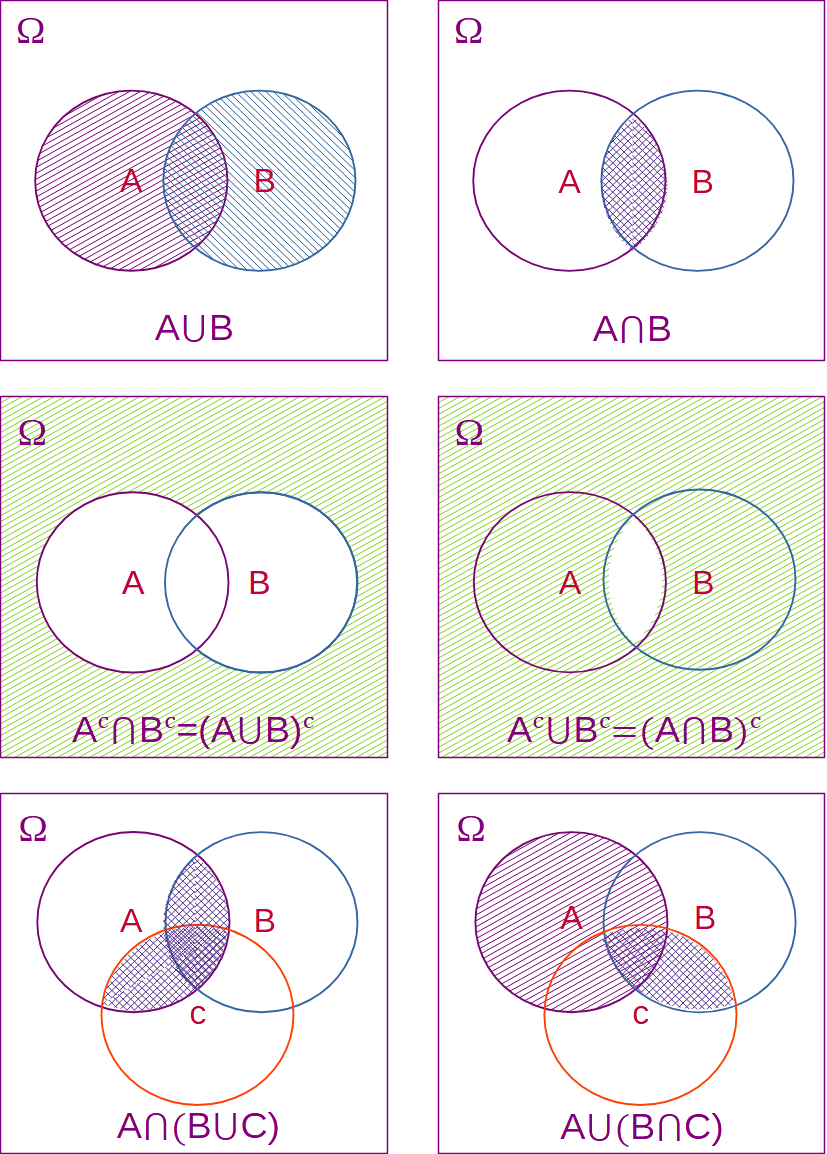
\includegraphics[width=5.30208in,height=\textheight]{Vennd.png}

}

\caption{\label{fig-venn}Diagramas de Venn}

\end{figure}%

Algunas de las leyes mencionadas anteriormente se ilustran en los
diagramas de Venn en la Figura~\ref{fig-venn}. Aunque se utilizará
libremente cualquiera de las leyes mencionadas, podría resultar
instructivo proporcionar una prueba de una de ellas para ilustrar la
técnica. Se considera el siguiente ejemplo:

\begin{tcolorbox}[enhanced jigsaw, titlerule=0mm, left=2mm, opacityback=0, toprule=.15mm, colframe=quarto-callout-caution-color-frame, bottomrule=.15mm, breakable, coltitle=black, opacitybacktitle=0.6, bottomtitle=1mm, colback=white, arc=.35mm, leftrule=.75mm, toptitle=1mm, colbacktitle=quarto-callout-caution-color!10!white, title={Ejemplo}, rightrule=.15mm]

Demostrar que \((A \cup B)^c = A^c \cap B^c\).

\begin{proof}
Según la definición, dos conjuntos son iguales si cada uno está
contenido en el otro. Primero se demuestra que
\((A\cup B)^c \subset A^c\cap B^c\) al probar que si
\(\omega \in (A\cup B)^c\), entonces \(\omega \in A^c \cap B^c\). Ahora
bien, \(\omega \in (A\cup B)^c\) implica que \(\omega \notin A \cup B\),
lo cual implica que \(\omega \notin A\) y \(\omega \notin B\), lo que a
su vez implica que \(\omega \in A^c\) y \(\omega \in B^c\); es decir,
\(\omega \in A^c\cap B^c\). A continuación se demuestra que
\(A^c \cap B^c \subset (A\cup B)^c\). Sea \(\omega \in A^c \cap B^c\),
lo que significa que \(\omega\) pertenece tanto a \(A^c\) como a
\(B^c\). Entonces, \(\omega \notin A \cup B\), ya que de lo contrario
\(\omega\) debería pertenecer al menos a uno de los conjuntos \(A\) o
\(B\), lo cual contradice que \(\omega\) pertenezca tanto a \(A^c\) como
a \(B^c\); sin embargo, \(\omega \notin A \cup B\) implica que
\(\omega \in (A\cup B)^c\), lo que completa la prueba.
\end{proof}

\end{tcolorbox}

Se han definido la unión y la intersección de dos conjuntos; estas
definiciones se extienden inmediatamente a más de dos conjuntos, de
hecho, a un número arbitrario de conjuntos. Es costumbre distinguir
entre los conjuntos en una colección de subconjuntos de \(\Omega\)
asignándoles nombres en forma de subíndices.

Se considera el conjunto de índices \(\Lambda\) como el catálogo de
nombres o índices. A \(\Lambda\) también se le denomina conjunto de
índices. Por ejemplo, si se tiene interés únicamente en dos conjuntos,
entonces el conjunto de índices \(\Lambda\) incluye solo dos índices,
por ejemplo, 1 y 2; así, \(\Lambda=\{1,2\}\).

\begin{definition}[Unión e intersección de
conjuntos]\protect\hypertarget{def-UI}{}\label{def-UI}

Sea \(\Lambda\) un conjunto de índices y
\(\{A_\lambda: \lambda \in \Lambda\}= \{A_\lambda\}\), una colección de
subconjuntos de \(\Omega\) indexados por \(\Lambda\). El conjunto de
puntos que consiste en todos los puntos que pertenecen a \(A_\lambda\)
para al menos un \(\lambda\) se denomina unión de los conjuntos
\(\{A_\lambda\}\) y se denota como
\(\bigcup\limits_{\lambda\in \Lambda} A_\lambda\). El conjunto de puntos
que consiste en todos los puntos que pertenecen a \(A_\lambda\) para
cada \(\lambda\) se denomina intersección de los conjuntos
\(\{A_\lambda\}\) y se denota como
\(\bigcap\limits_{\lambda\in\Lambda} A_\lambda\). Si \(\Lambda\) está
vacío, entonces se define
\(\bigcup\limits_{\lambda\in \Lambda} A_\lambda = \emptyset\) y
\(\bigcap\limits_{\lambda\in\Lambda} A_\lambda=\Omega\).

\end{definition}

Uno de los teoremas más fundamentales que relaciona las uniones,
intersecciones y complementos para una colección arbitraria de conjuntos
se debe a De Morgan.

\begin{theorem}[Teorema de De
Morgan]\protect\hypertarget{thm-morgan}{}\label{thm-morgan}

Sea \(\Lambda\) un conjunto de índices y \(\{A_\lambda\}\) una colección
de subconjuntos de \(\Omega\) indexados por \(\Lambda\). Entonces,

\begin{enumerate}
\def\labelenumi{\roman{enumi}.}
\item
  \(\left(\bigcup\limits_{\lambda\in\Lambda} A_\lambda\right)^c = \bigcap\limits_{\lambda\in\Lambda} A_\lambda^c\)
\item
  \(\left(\bigcap\limits_{\lambda\in\Lambda} A_\lambda\right)^c = \bigcup\limits_{\lambda\in\Lambda} A_\lambda^c\)
\end{enumerate}

\end{theorem}

\begin{definition}[Disjuntos o mutuamente
excluyentes]\protect\hypertarget{def-disjunto}{}\label{def-disjunto}

Los subconjuntos \(A\) y \(B\) de \(\Omega\) se definen como mutuamente
excluyentes o disjuntos si \(A\cap B=\emptyset\). Los subconjuntos
\(A_1, A_2, \ldots\) se definen como mutuamente excluyentes si
\(A_i\cap A_j=\emptyset\) para cada \(i\neq j\).

\end{definition}

\chapter{Probabilidad}\label{probabilidad}

Una de las herramientas fundamentales de la estadística es la
probabilidad, la cual tuvo sus inicios formales con los juegos de azar
en el siglo XVII. Los juegos de azar, como su nombre indica, involucran
acciones como girar una rueda de ruleta, lanzar dados, lanzar una
moneda, sacar una carta, entre otros, en los que el resultado de un
evento es incierto. No obstante, se reconoce que aunque el resultado de
cada evento en particular pueda ser incierto, existe un patrón
predecible a largo plazo. Por ejemplo, se sabe que en múltiples
lanzamientos de una moneda ideal (equilibrada y simétrica),
aproximadamente la mitad de los resultados serán caras. Es esta
regularidad predecible a largo plazo la que permite a las casas de juego
mantener sus negocios.

Un tipo similar de incertidumbre y regularidad a largo plazo se observa
con frecuencia en la ciencia experimental. Por ejemplo, en la ciencia de
la genética no se puede determinar con certeza si una descendencia será
masculina o femenina, pero a largo plazo se sabe aproximadamente qué
porcentaje de descendencia será de cada sexo. De manera similar, una
compañía de seguros de vida no puede predecir qué personas en los
Estados Unidos morirán a los 50 años, pero puede hacer predicciones
precisas sobre cuántas personas morirán a esa edad en promedio.

Para brindar una idea de lo que es la probabilidad, (Mood, Graybill, y
Boes 1986) proporciona las siguientes definiciones:

\begin{definition}[Probabilidad
clásica]\protect\hypertarget{def-pclas}{}\label{def-pclas}

Si un experimento aleatorio puede resultar en \(n\) resultados
mutuamente excluyentes e igualmente probables y si \(s\) de estos
resultados tienen un atributo \(A\), entonces la probabilidad de \(A\)
es la fracción \(s/n\).

\end{definition}

\begin{definition}[Probabilidad
frecuentista]\protect\hypertarget{def-pfrec}{}\label{def-pfrec}

Suponiendo que después de \(n\) repeticiones, para valores muy grandes
de \(n\), un evento \(A\) puede ocurrir \(s\) veces. Entonces \(p=s/n\).

\end{definition}

Estas definiciones, a pesar de su intuición, presentan limitaciones
significativas. Por ejemplo, la primera definición es circular, ya que
la frase ``igualmente probables'' es justamente lo que se intenta
definir. Además, la segunda definición no especifica los valores de
\(n\), lo cual puede generar ambigüedad. Estas definiciones son
consideradas antiguas, pero aún pueden brindar una comprensión general
del concepto de \textbf{probabilidad}.

\section{Espacio muestral y eventos}\label{espacio-muestral-y-eventos}

A continuación, se presentarán algunas definiciones que resultarán de
gran utilidad para adquirir un mayor conocimiento sobre el concepto de
probabilidad. Se usará como referencia (Lipschutz 1996).

\begin{definition}[Espacio
muestral]\protect\hypertarget{def-espm}{}\label{def-espm}

El espacio muestral, denotado por \(\Omega\), es la colección o
totalidad de todos los posibles resultados de un experimento conceptual.

\end{definition}

Un resultado particular, es decir, un elemento del espacio muestral
\(\Omega\), se denomina un \textbf{\emph{punto muestral}} o una
\textbf{\emph{muestra}}.

\begin{definition}[Evento]\protect\hypertarget{def-evento}{}\label{def-evento}

Un evento \(A\) es un subconjunto del espacio muestral \(\Omega\), es
decir, es un conjunto de resultados.

\end{definition}

\begin{definition}[Espacio de
eventos]\protect\hypertarget{def-espev}{}\label{def-espev}

La clase de todos los eventos asociados a un experimento dado se define
como el espacio de eventos y se denotará por \(\mathfrak{F}\).

\end{definition}

\begin{definition}[Evento
particular]\protect\hypertarget{def-evpart}{}\label{def-evpart}

El evento \(\{\omega\}\), que está constituido por un solo punto
\(\omega \in \Omega\), se denomina \emph{evento muestral} o \emph{punto
muestral}.

\end{definition}

Las definiciones anteriores no definen con precisión lo que es un
evento. Un evento siempre será un subconjunto del espacio muestral, pero
para espacios muestrales suficientemente grandes, no todos los
subconjuntos serán eventos. Por lo tanto, la clase de todos los
subconjuntos del espacio muestral no necesariamente corresponderá al
espacio de eventos. Sin embargo, se observará que la clase de todos los
eventos siempre se puede seleccionar lo suficientemente grande como para
incluir todos aquellos subconjuntos (eventos) cuya probabilidad se desee
analizar. Si el espacio muestral consta solo de un número finito de
puntos, entonces el espacio de eventos correspondiente será la clase de
todos los subconjuntos del espacio muestral.

Los conceptos presentados se ilustran con unos ejemplos muy simples;

\begin{tcolorbox}[enhanced jigsaw, titlerule=0mm, left=2mm, opacityback=0, toprule=.15mm, colframe=quarto-callout-caution-color-frame, bottomrule=.15mm, breakable, coltitle=black, opacitybacktitle=0.6, bottomtitle=1mm, colback=white, arc=.35mm, leftrule=.75mm, toptitle=1mm, colbacktitle=quarto-callout-caution-color!10!white, title={Ejemplo (\textbf{\emph{Lanzamiento de una moneda}})}, rightrule=.15mm]

Considerando el experimento de lanzar una moneda, este experimento es
uno de los más sencillos, pero permite representar claramente los
conceptos. El espacio muestral estaría conformado por
\(\Omega = \{A, S\}\), donde \(A\) representa el resultado de que caiga
águila y \(S\) representa el resultado de que caiga sol. El conjunto
\(\mathfrak{F}\) podría estar representado por \(\{\{A\}, \{S\}\}\), que
también es un subconjunto de \(\Omega\).

Es importante destacar que el conjunto vacío \(\emptyset\) y el conjunto
completo \(\Omega\) también son subconjuntos de \(\Omega\), pero
generalmente no se consideran eventos de interés en este contexto.

\end{tcolorbox}

\begin{tcolorbox}[enhanced jigsaw, titlerule=0mm, left=2mm, opacityback=0, toprule=.15mm, colframe=quarto-callout-caution-color-frame, bottomrule=.15mm, breakable, coltitle=black, opacitybacktitle=0.6, bottomtitle=1mm, colback=white, arc=.35mm, leftrule=.75mm, toptitle=1mm, colbacktitle=quarto-callout-caution-color!10!white, title={Ejemplo (\textbf{\emph{Lanzamiento de un dado}})}, rightrule=.15mm]

Considerando el experimento de lanzar un dado de \(6\) caras. El espacio
muestral \(\Omega\) se define como

\[ \Omega = \{1,2,3,4,5,6\}. \]

Un punto muestral podría ser un resultado específico, por ejemplo,
\(\{1\}\). Todos los subconjuntos posibles de resultados constituirían
el conjunto \(\mathfrak{F}\). Se definen los eventos \(A\), que
representa el evento de obtener un resultado par; \(B\), que representa
el evento de obtener un resultado impar; y \(C\), que representa el
evento de obtener un resultado mayor a 3. Por lo tanto, se tiene:

\[ A= \{2,4,6\},\quad B=\{1,3,5\},\quad C=\{4,5,6\}. \]

Se observa que el evento de la unión de los eventos \(B\) y \(C\),
denotado como \(B\cup C\), es igual a \(\{1, 3, 4, 5, 6\}\), el cual
también es un evento en el espacio muestral \(\Omega\). Finalmente, se
destaca que los eventos \(A\) y \(B\) no tienen elementos en común, es
decir, \(A \cap B = \emptyset\). Por lo tanto, se dice que estos eventos
son ajenos, mutuamente excluyentes o disjuntos.

\end{tcolorbox}

La definición de espacio muestral es precisa y satisfactoria, mientras
que las definiciones de evento y espacio de eventos no son completamente
satisfactorias. Se mencionó que si el espacio muestral era
``suficientemente grande'', no todos los subconjuntos del espacio
muestral serían eventos; sin embargo, no se especificó exactamente qué
subconjuntos serían eventos y cuáles no lo serían. En lugar de
desarrollar las matemáticas necesarias para definir con precisión qué
subconjuntos de \(\Omega\) constituyen nuestro espacio de eventos
\(\mathfrak{F}\), se pueden enunciar algunas propiedades de
\(\mathfrak{F}\) que parecen razonables requerir.

\begin{enumerate}
\def\labelenumi{\roman{enumi}.}
\item
  \(\Omega \in \mathfrak{F}\).
\item
  Si \(A\in\mathfrak{F}\), entonces \(A^c\in \mathfrak{F}\).
\item
  Si \(A_1\) y \(A_2\in \mathfrak{F}\), entonces
  \(A_1\cup A_2\in \mathfrak{F}\).
\end{enumerate}

Se mencionó anteriormente que el interés principal radica en los eventos
debido a la probabilidad de que ocurran. Por lo tanto, es deseable que
\(\mathfrak{F}\) incluya \(\Omega\), el evento seguro. Además, si \(A\)
es un evento, lo que significa que se puede hablar sobre la probabilidad
de que ocurra \(A\), entonces \(A^c\) también debería ser un evento para
poder hablar sobre la probabilidad de que \(A\) no ocurra. De manera
similar, si \(A_1\) y \(A_2\) son eventos, entonces \(A_1\cup A_2\)
también debería ser un evento.

Cualquier colección de eventos con propiedades (i.) y (iii.) se denomina
álgebra booleana, o simplemente álgebra, de eventos. Cabe señalar que la
colección de todos los subconjuntos de \(\Omega\) satisface
necesariamente las propiedades mencionadas anteriormente. Varios
resultados se derivan de las propiedades asumidas anteriormente de
\(\mathfrak{F}\).

\section{Definición de
probabilidad}\label{definiciuxf3n-de-probabilidad}

En esta sección se presenta la definición axiomática de probabilidad.
Aunque esta definición formal de probabilidad por sí sola no permite
asignar probabilidades reales a eventos que consisten en ciertos
resultados de experimentos aleatorios, es otra de una serie de
definiciones que conducen a ese objetivo. Dado que la probabilidad, al
igual que los conceptos que se presentarán, se define como una función
particular, se inicia esta subsección con una revisión del concepto de
función

\begin{definition}[Función]\protect\hypertarget{def-funcion}{}\label{def-funcion}

Una función, llamada \(f(\cdot)\), con dominio \(A\) y contradominio
\(B\), es una colección de pares ordenados, llamados \((a,b)\), que
cumplen las siguientes condiciones:

\begin{enumerate}
\def\labelenumi{\roman{enumi}.}
\item
  \(a\in A\) y \(b\in B\)
\item
  Cada \(a\in A\) aparece como el primer elemento de algún par ordenado
  en la colección (cada \(b\in B\) no necesariamente es el segundo
  elemento de algún par ordenado)
\item
  Ningún par ordenado en la colección tiene el mismo primer elemento que
  otro par ordenado distinto.
\end{enumerate}

\end{definition}

Si \((a,b)\in f(\cdot)\), se escribe \(b=f(a)\) (se lee ``\(b\) es igual
a \(f\) de \(a\)'') y se denomina \(f(a)\) como el valor de \(f(\cdot)\)
en \(a\). Para cualquier \(a\in A\), \(f(a)\) es un elemento de \(B\);
mientras que \(f(\cdot)\) es un conjunto de pares ordenados. El conjunto
de todos los valores de \(f(\cdot)\) se denomina rango de \(f(\cdot)\);
es decir, el rango de
\(f(\cdot)=\{b\in B:b=f(a) \text{ para algún } a\in A\}\) y siempre es
un subconjunto del contradominio \(B\), pero no necesariamente igual a
él. \(f(a)\) también se denomina imagen de \(a\) bajo \(f(\cdot)\), y
\(a\) se denomina preimagen de \(f(a)\).

\begin{tcolorbox}[enhanced jigsaw, titlerule=0mm, left=2mm, opacityback=0, toprule=.15mm, colframe=quarto-callout-caution-color-frame, bottomrule=.15mm, breakable, coltitle=black, opacitybacktitle=0.6, bottomtitle=1mm, colback=white, arc=.35mm, leftrule=.75mm, toptitle=1mm, colbacktitle=quarto-callout-caution-color!10!white, title={Ejemplo}, rightrule=.15mm]

Sean \(f_1(\cdot)\) y \(f_2(\cdot)\) dos funciones con la recta real
como su dominio y contradominio, definidas por

\[ f_1(\cdot)=\{(x,y): y=x^3+1, -\infty< x< \infty\} \]

y

\[ f_2(\cdot)=\{(x,y): y=x^2, -\infty<x< \infty\} \]

El rango de \(f_1(\cdot)\) es el contradominio, que es toda la recta
real, pero el rango de \(f_2(\cdot)\) son todos los números reales no
negativos, que no es igual al contradominio.

\end{tcolorbox}

De particular interés será una clase de funciones conocidas como
funciones indicadoras.

\begin{definition}[Función
indicadora]\protect\hypertarget{def-f_ind}{}\label{def-f_ind}

Sea \(\Omega\) cualquier espacio con puntos \(\omega\) y \(A\) cualquier
subconjunto de \(\Omega\). La función indicadora de \(A\), denominada
\(I_A(\cdot)\), es la función con dominio \(\Omega\) y contradominio
formado por dos números reales, 0 y 1, definida por

\[ I_A(\omega)= \left\{\begin{array}{lcc} 1 & si & \omega \in A\\ \\0 & si & \omega \notin A \end{array}\right. \]

\(I_A(\cdot)\) claramente ``indica'' el conjunto \(A\).

\end{definition}

\textbf{\emph{Propiedades de la función indicadora.}}

Sea \(\Omega\) cualquier espacio y \(\mathfrak{F}\) cualquier colección
de subconjuntos de \(\Omega\):

\begin{enumerate}
\def\labelenumi{\roman{enumi}.}
\item
  \(I_A(\omega)= 1- I_{A^c}(\omega)\) para cada \(A\in \mathfrak{F}\).
\item
  \(I_{A_1A_2\cdots A_n}(\omega)= I_{A_1}(\omega)\cdot I_{A_2}(\omega)\cdots I_{A_n}(\omega)\)
  para \(A_1,\ldots, A_n\in \mathfrak{F}\).
\item
  \(I_{A_1\cup A_2\cup\cdots\cup A_n}(\omega)= \max{[I_{A_1}(\omega), I_{A_2}(\omega),\ldots, I_{A_n}(\omega)]}\)
  para \(A_1, \ldots, A_n \in\mathfrak{F}\).
\item
  \(I_A^2(\omega)= I_A(\omega)\) para cada \(A\in\mathfrak{F}\).
\end{enumerate}

La función indicadora será utilizada para ``indicar'' subconjuntos de la
recta real; por ejemplo;

\[I_{\{[0,1)\}}(x)= I_{[0,1)}(x)=\left\{ \begin{array}{lcc} 1 & \text{si} & 0\leq x<1\\ \\ 0 & \text{ otro caso} \end{array} \right. \]

y si \(I^+\) denota el conjunto de números enteros positivos,

\[ I_{I^+}(X)=\left\{\begin{array}{lcc} 1 & \text{si $x$ es algún entero positivo}\\ \\ 0 & \text{otro caso}\end{array}\right. \]

Otro tipo de función del cual se tendrá ocasión de discutir es la
función de conjunto definida como cualquier función que tiene como
dominio una colección de conjuntos y como contradominio la recta real,
incluyendo posiblemente el infinito. A continuación se muestra un
ejemplos de función de conjunto.

\begin{tcolorbox}[enhanced jigsaw, titlerule=0mm, left=2mm, opacityback=0, toprule=.15mm, colframe=quarto-callout-caution-color-frame, bottomrule=.15mm, breakable, coltitle=black, opacitybacktitle=0.6, bottomtitle=1mm, colback=white, arc=.35mm, leftrule=.75mm, toptitle=1mm, colbacktitle=quarto-callout-caution-color!10!white, title={Ejemplo}, rightrule=.15mm]

Sea \(\Omega\) el espacio muestral correspondiente al experimento de
lanzar dos dados, y sea \(\mathfrak{F}\) la colección de todos los
subconjuntos de \(\Omega\). Para cualquier \(A\in\mathfrak{F}\), se
define \(N(A)\) como el número de resultados, o puntos en \(\Omega\),
que están en \(A\). Entonces, \(N(\emptyset)=0\), \(N(\Omega)=36\) y
\(N(A)=6\) si \(A\) es el evento que contiene aquellos resultados que
tienen un total de siete puntos arriba.

\end{tcolorbox}

La función de tamaño del conjunto aludida en el ejemplo anterior puede
ser definida, en general, para cualquier conjunto \(A\) como el número
de puntos en \(A\), donde \(A\) es un miembro de una colección
arbitraria de conjuntos \(\mathfrak{F}\).

La función de probabilidad que se definirá será una función de conjunto
particular.

\begin{definition}[Función de
probabilidad]\protect\hypertarget{def-fprob}{}\label{def-fprob}

Sea \(A\) un evento del espacio muestral \(\Omega\). Una función
\(P: \mathfrak{F} \to [0,1]\) es llamada función de probabilidad y
\(P(A)\) se denomina la \emph{probabilidad} del evento \(A\) si se
cumplen los siguientes axiomas:

\begin{enumerate}
\def\labelenumi{\roman{enumi}.}
\item
  \textbf{\emph{No negatividad}}: Para todo evento \(A\) en
  \(\mathfrak{F}\), la probabilidad \(P(A)\) es un número no negativo,
  es decir, \(P(A) \geq 0\).
\item
  \textbf{\emph{Probabilidad unitaria}}: La probabilidad del espacio
  muestral completo \(\Omega\) es igual a 1, es decir,
  \(P(\Omega) = 1\).
\item
  \textbf{\emph{Aditividad}}: Para cualquier colección de eventos
  mutuamente excluyentes \(A_1, A_2, A_3, \ldots\), la probabilidad de
  la unión de estos eventos es igual a la suma de las probabilidades
  individuales, es decir,
  \[P\left(\bigcup_{i=1}^\infty A_i\right) = \sum_{i=1}^\infty P(A_i)\]
\end{enumerate}

\end{definition}

Estos axiomas establecen las propiedades esenciales que debe cumplir una
función de probabilidad para ser considerada válida. Cumplir con estos
axiomas garantiza que la función de probabilidad asigna valores
coherentes y consistentes a los eventos en el espacio muestral.

A partir de los axiomas, se derivan otras propiedades que nos ayudarán a
posible calcular las probabilidades de varios eventos.

\begin{enumerate}
\def\labelenumi{\roman{enumi}.}
\item
  \(P(\emptyset)=0\).
\item
  Si \(A_1, \ldots, A_n\) son eventos mutuamente excluyentes en
  \(\mathfrak{F}\), entonces
  \[P\left(\bigcup\limits_{i=1}^n A_i\right)= \sum\limits_{i=1}^n P(A_i).\]
\item
  Si \(A\) es un evento en \(\mathfrak{F}\), entonces
  \[P(A^c)= 1-P(A).\]
\item
  Si \(A,B\in\mathfrak{F}\), entonces

  \[P(A)= P(A\cap B)+ P(A\cap B^c)\]

  y \[P(A-B)=P(A\cap B^c)= P(A)-P(A\cap B).\]
\item
  Si \(A,B\in \mathfrak{F}\) y \(A\subset B\), entonces
  \(P(A)\leq P(B)\).
\item
  Para cualesquiera dos eventos \(A,B\in \mathfrak{F}\);
  \[P(A\cup B)= P(A)+P(B)-P(A\cap B).\]Más generalmente, para eventos
  \(A_1, A_2, \ldots, A_n\in \mathfrak{F}\)
\end{enumerate}

\[ P\left(\bigcup\limits_{i=1}^n A_i\right) = \sum_{j=1}^nP(A_j)-{\sum\sum}_{i<j} P(A_i\cap A_j)+\sum\sum\sum_{i<j<k}P(A_i\cap A_j\cap A_k)\\ -\cdots+(-1)^{n+1}P(A_1\cap \ldots\cap A_n) \]

\begin{theorem}[Desigualdad de
Boole]\protect\hypertarget{thm-boole}{}\label{thm-boole}

Si \(A_1, A_2, \ldots, A_n\in\mathfrak{F}\), entonces

\[P\left(\bigcup_{i=1}^n A_i\right)\leq \sum_{i=1}^n P(A_i)\]

\end{theorem}

Finalmente se concluye esta subsección con la siguiente definición;

\begin{definition}[Espacio de
probabilidad]\protect\hypertarget{def-Ep}{}\label{def-Ep}

Un espacio de probabilidad es la terna \((\Omega, \mathfrak{F}, P)\),
donde \(\Omega\) es un espacio muestral, \(\mathfrak{F}\) es una
colección (asumida como un álgebra) de eventos (cada uno un subconjunto
de \(\Omega\)), y \(P\) es una función de probabilidad con dominio
\(\mathfrak{F}\).

\end{definition}

\section{Probabilidad condicional}\label{probabilidad-condicional}

En ocasiones, es de interés conocer la probabilidad de un evento, dado
que haya ocurrido otro. En este sentido, se define la probabilidad
condicional.

\begin{definition}[Probabilidad
condicional]\protect\hypertarget{def-pcond}{}\label{def-pcond}

Sean \(A\) y \(B\) dos eventos en \(\mathfrak{F}\) del espacio de
probabilidad dado \((\Omega, \mathfrak{F}, P)\). La probabilidad
condicional del evento \(A\) dado el evento \(B\), denotada por
\(P(A|B)\), se define como sigue;

\[P(A|B)= \frac{P(A\cap B)}{P(B)}\qquad\text{si }\quad P(B)>0,\]

y se deja sin definir si \(P(B)=0\).

\end{definition}

\begin{remark}
Una fórmula que es evidente a partir de la definición es
\[P(A\cap B)= P(A|B)P(B)=P(B|A)P(A)\] si tanto \(P(A)\) como \(P(B)\)
son diferentes de cero. Esta fórmula relaciona \(P(A|B)\) con \(P(B|A)\)
en términos de las probabilidades incondicionales \(P(A)\) y \(P(B)\).
\end{remark}

De la definición anterior, se desprenden las siguientes propiedades de
la función de probabilidad condicional. Se asume que el espacio de
probabilidad \((\Omega, \mathfrak{F}, P)\) está dado, y se considera que
\(B\in\mathfrak{F}\) cumple con \(P[B]>0\).

\begin{enumerate}
\def\labelenumi{\roman{enumi}.}
\item
  \(P(\emptyset| B)=0\).
\item
  Si \(A_1, A_2, \ldots, A_n\) son eventos mutuamente excluyentes en
  \(\mathfrak{F}\), entonces

  \[P\left(\bigcup_{i=1}^n A_i|B\right)= \sum_{i=1}^n P(A_i|B).\]
\item
  Si \(A\) es un evento en \(\mathfrak{F}\), entonces
  \(P(A^c| B)=1-P(A|B)\).
\item
  Si \(A_1, A_2\in \mathfrak{F}\), entonces
  \(P(A_1|B)=P(A_1\cap A_2|B)+ P(A_1\cap A_2^c|B)\).
\item
  Para cualesquiera dos eventos \(A_1,A_2\in \mathfrak{F}\)

  \[P(A_1\cup A_2|B)=P(A_1|B)+P(A_2|B)-P(A_1\cap A_2|B).\]
\item
  Si \(A_1, A_2\in\mathfrak{F}\) y \(A_1\subset A_2\), entonces
  \(P(A_1|B)\leq P(A_2|B)\).
\item
  Si \(A_1, A_2,\ldots, A_n\in\mathfrak{F}\), entonces

  \[P\left(\bigcup_{i=1}^n A_i|B\right)\leq \sum_{i=1}^n P(A_i|B).\]
\end{enumerate}

A continuación se mencionan unos teoremas de gran importancia. La
aplicación de dichos teoremas se ilustran con unos ejemplos.

\begin{theorem}[Teorema de probabilidades
totales]\protect\hypertarget{thm-ptotales}{}\label{thm-ptotales}

Para un espacio de probabilidad dado \((\Omega, \mathfrak{F}, P)\), si
\(B_1, B_2, \ldots, B_n\) es una colección de eventos mutuamente
disjuntos en \(\mathfrak{F}\) que satisfacen
\(\Omega = \bigcup\limits_{j=1}^n B_j\) y \(P(B_j)>0\) para
\(j=1,\ldots, n\), entonces para cada \(A\in \mathfrak{F}\),
\[P(A)=\sum_{j=1}^n P(A|B_j)P(B_j).\]

\begin{proof}
Se observa que \(A=\bigcup\limits_{j=1}^n A\cap B_j\) y los conjuntos
\(A\cap B_j\) son mutuamente disjuntos; por lo tanto,

\[P(A)=P\left(\bigcup_{j=1}^n A\cap B_j\right)=\sum_{j=1}^n P(A\cap B_j)= \sum_{j=1}^n P(A|B_j)P(B_j)\]
\end{proof}

\end{theorem}

\begin{tcolorbox}[enhanced jigsaw, titlerule=0mm, left=2mm, opacityback=0, toprule=.15mm, colframe=quarto-callout-caution-color-frame, bottomrule=.15mm, breakable, coltitle=black, opacitybacktitle=0.6, bottomtitle=1mm, colback=white, arc=.35mm, leftrule=.75mm, toptitle=1mm, colbacktitle=quarto-callout-caution-color!10!white, title={Ejemplo (\textbf{\emph{Seleccionar una pelota de varias urnas}})}, rightrule=.15mm]

Hay dos urnas con pelotas de diferentes colores, todas del mismo tamaño.
En la primera urna, hay tres pelotas rojas, tres blancas y cuatro
negras; en la segunda urna, hay cuatro pelotas rojas, tres blancas y una
negra. Se elige una urna al azar y se saca una pelota de ella. ¿Cuál es
la probabilidad de que la pelota extraída sea blanca?

\begin{solution}
Se debe observar que la elección de las urnas constituye dos eventos
mutuamente excluyentes, ya que la unión de ambos eventos constituye el
espacio muestral (todas las pelotas están en la primera o segunda urna).
Se denomina \(B_1\) al evento de seleccionar la primera urna, y \(B_2\)
al evento de seleccionar la segunda urna.

El evento de extraer una pelota blanca puede tener lugar tanto al elegir
la primera urna como al elegir la segunda urna, lo que permite la
aplicación de la fórmula del teorema de probabilidades totales. Se
designa como \(A\) al evento de seleccionar una pelota blanca.

De esta manera,

\[ P(A)= \sum_{j=1}^2 P(A|B_j)P(B_j)=P(A|B_1)P(B_1)+P(A|B_2)P(B_2) \]

Bajo la premisa de probabilidades equivalentes, se tiene que
\(P(B_1)=P(B_2)=\frac{1}{2}\), \(P(A|B_1)=\frac{3}{10}\) y
\(P(A|B_2)=\frac{3}{8}\), por lo que la probabilidad de elegir una
pelota blanca es \(0.3375\).
\end{solution}

\end{tcolorbox}

\begin{theorem}[Teorema de
Bayes]\protect\hypertarget{thm-bayes}{}\label{thm-bayes}

Para un espacio de probabilidad dado \((\Omega, \mathfrak{F}, P)\), si
\(B_1, B_2, \ldots, B_n\) es una colección de eventos mutuamente
disjuntos en \(\mathfrak{F}\) que satisfacen
\(\Omega=\bigcup\limits_{j=1}^n B_j\) y \(P(B_j)>0\) para
\(j=1,\ldots, n\), entonces para cada \(A\in\mathfrak{F}\) para el cual
\(P(A)>0\)

\[P(B_k|A)= \frac{P(A|B_k)P(B_k)}{\sum\limits_{j=1}^n P(A|B_j)P(B_j)}.\]

\begin{proof}
Se observa que

\[P(B_k|A)= \frac{P(B_k\cap A)}{P(A)}=\frac{P(A|B_k)P(B_k)}{\sum\limits_{j=1}^n P(A|B_j)P(B_j)}\]

utilizando tanto la definición de probabilidad condicional como el
teorema de probabilidad total.
\end{proof}

\end{theorem}

\begin{tcolorbox}[enhanced jigsaw, titlerule=0mm, left=2mm, opacityback=0, toprule=.15mm, colframe=quarto-callout-caution-color-frame, bottomrule=.15mm, breakable, coltitle=black, opacitybacktitle=0.6, bottomtitle=1mm, colback=white, arc=.35mm, leftrule=.75mm, toptitle=1mm, colbacktitle=quarto-callout-caution-color!10!white, title={Ejemplo (\textbf{\emph{Seleccionar una pelota de varias urnas}})}, rightrule=.15mm]

Considérese el problema de las urnas. Teniendo en cuenta que la pelota
extraída fue blanca, ¿cuál es la probabilidad de que haya provenido de
la primera urna?

\begin{solution}
Debe calcularse la probabilidad \(P(B_1|A)\). Al utilizar el teorema de
Bayes, solo se realiza la sustitución en la fórmula y se obtiene que la
probabilidad resultante es \(0.4444\).
\end{solution}

\end{tcolorbox}

\begin{theorem}[Regla de
multiplicación]\protect\hypertarget{thm-mult}{}\label{thm-mult}

Para un espacio de probabilidad dado \((\Omega, \mathfrak{F}, P)\), sean
\(A_1, A_2, \ldots, A_n\) eventos pertenecientes a \(\mathfrak{F}\) para
los cuales \(P(A_1\cdots A_{n-1})>0\); entonces

\[P(A_1A_2\cdots A_n)= P(A_1)P(A_2|A_1)P(A_3|A_1A_2)\cdots P(A_n|A_1\cdots A_{n-1})\]

\end{theorem}

\section{Independencia de eventos}\label{independencia-de-eventos}

Si \(P(A|B)\) no depende del evento \(B\), es decir, \(P(A|B)=P(A)\),
entonces parecería natural decir que el evento \(A\) es independiente
del evento \(B\). Esto se establece en la siguiente definición.

\begin{definition}[Eventos
independientes]\protect\hypertarget{def-evind}{}\label{def-evind}

Para un espacio de probabilidad dado \((\Omega, \mathfrak{F}, P)\), sean
\(A\) y \(B\) dos eventos en \(\mathfrak{F}\). Los eventos \(A\) y \(B\)
se definen como \emph{independientes} si y solo si se cumple alguna de
las siguientes condiciones:

\begin{enumerate}
\def\labelenumi{\roman{enumi}.}
\item
  \(P(A\cap B)= P(A)P(B)\).
\item
  \(P(A|B)=P(A)\) si \(P(B)>0\).
\item
  \(P(B|A)=P(B)\) si \(P(A)>0\).
\end{enumerate}

\end{definition}

De la definición anterior, se desprende lo siguiente

\phantomsection\label{thm}
Si \(A\) y \(B\) son dos eventos independientes definidos en un espacio
de probabilidad dado \((\Omega, \mathfrak{F}, P)\), entonces los
siguientes eventos también son independientes

\begin{enumerate}
\def\labelenumi{\roman{enumi}.}
\item
  \(A\) y \(B^c\),
\item
  \(A^c\) y \(B\),
\item
  \(A^c\) y \(B^c\).
\end{enumerate}

\begin{remark}
No debe confundirse los términos \textbf{eventos independientes} y
\textbf{eventos disjuntos}. De hecho, los eventos disjuntos suelen ser
muy dependientes por que la ocurrencia de uno implica la no ocurrencia
del otro. El único evento que es independiente y ajeno es el vacío
\(\emptyset\).
\end{remark}

La noción de eventos independientes puede ser extendido a más de dos
eventos como se sigue;

\begin{definition}[Independencia de varios
eventos]\protect\hypertarget{def-ive}{}\label{def-ive}

Para un espacio de probabilidad dado \((\Omega, \mathfrak{F}, P)\), sean
\(A_1, A_2, \ldots, A_n\) eventos en \(\mathfrak{F}\). Los eventos
\(A_1, A_2, \ldots, A_n\) se definen como independientes si y solo si
\(P\left(\bigcap\limits_{i=1}^n A_i\right)=\prod\limits_{i=1}^n P(A_i)\)

\end{definition}

\section{Variables aleatorias}\label{variables-aleatorias}

Hasta el momento se conoce cómo asignar probabilidades a eventos del
espacio muestral, sin embargo en la práctica esto no siempre es posible
ya que sería complicado mencionar o enumerar todos los elementos del
espacio muestral.

Por esta razón es necesario ``traducir'' dichos eventos a números
reales. Esto es posible mediante el uso de \emph{variables aleatorias}.

\begin{definition}[Variable
aleatoria]\protect\hypertarget{def-va}{}\label{def-va}

Para un espacio de probabilidad dado \((\Omega, \mathfrak{F}, P)\), una
variable aleatoria, denotada por \(X\) o \(X(\cdot)\), es una función
con dominio \(\Omega\) y contradominio la recta real. La función
\(X(\cdot)\) debe ser tal si \(\omega\in\Omega\) entonces
\(X(\omega)\in\mathbb R\). Si \(B\subset \mathbb R\) entonces
\(X^{-1}(B)\in\mathfrak{F}\), donde
\[X^{-1}(B)=\{\omega\in\Omega| X(\omega\in B)\}.\]

\end{definition}

Existen dos tipos de variables aleatorias: discretas y continuas. Las
variables aleatorias discretas toman sus valores en un conjunto finito o
numerable, por ejemplo, el conjunto de los números naturales
\(\mathbb N\). A este conjunto de valores se le conoce como conjunto de
valores posibles o \(D_X\). Las variables aleatorias continuas, por el
contrario, toman sus valores en el conjunto de los números reales
\(\mathbb R\).

\subsection{Función de
distribución}\label{funciuxf3n-de-distribuciuxf3n}

Para describir el comportamiento de una variable aleatoria, se debe
conocer cómo se comportan sus probabilidades, esto puede realizarse
mediante la \emph{función de distribución}.

\begin{definition}[Función de distribución
acumulada]\protect\hypertarget{def-fundist}{}\label{def-fundist}

La función de distribución acumulada de una variable aleatoria \(X\),
denotada por \(F_X(\cdot)\), se define como aquella función con dominio
la recta real y contradominio el intervalo \([0,1]\), que satisface
\(F_X(x)=P(X\leq x)=P({\omega: X(\omega)\leq x})\) para cada número real
\(x\).

\end{definition}

Una función de distribución definida es única para cada variable y
siempre existirá, es importante conocerla por que con ella se pueden
calcular probabilidades de la variable aleatoria.

A continuación, se presentan ejemplos y propiedades de la función de
distribución acumulada.

\begin{tcolorbox}[enhanced jigsaw, titlerule=0mm, left=2mm, opacityback=0, toprule=.15mm, colframe=quarto-callout-caution-color-frame, bottomrule=.15mm, breakable, coltitle=black, opacitybacktitle=0.6, bottomtitle=1mm, colback=white, arc=.35mm, leftrule=.75mm, toptitle=1mm, colbacktitle=quarto-callout-caution-color!10!white, title={Ejemplo}, rightrule=.15mm]

Se considera el experimento de lanzar una moneda. Supongamos que la
moneda es justa. Sea \(X\) el número de caras obtenidas. Entonces,

\[F_X(x)=\left\{ \begin{array}{lcc} 0 & \text{si} & x<0\\ \\ \frac{1}{2} & \text{si} & 0\leq x<1 \\ \\1 & \text{si} & 1\leq x \end{array} \right. \]

O \(F_X(x)=\frac{1}{2}I_{[0,1)}(x)+ I_{[1,\infty)}(x)\) en nuestra
notación de función indicadora.

\end{tcolorbox}

\subsubsection{\texorpdfstring{\textbf{\emph{Propiedades de la función
de distribución
acumulada.}}}{Propiedades de la función de distribución acumulada.}}\label{propiedades-de-la-funciuxf3n-de-distribuciuxf3n-acumulada.}

\begin{enumerate}
\def\labelenumi{\roman{enumi}.}
\item
  \(F_X(-\infty)\equiv \lim\limits_{x\to-\infty} F_X(x)=0\), y
  \(F_X(+\infty)\equiv \lim\limits_{x\to+\infty} F_X(x)=1\).
\item
  \(F_X(\cdot)\) es una función monótona creciente; es decir, para toda
  \(a< b\) entonces \(F_X(a)\leq F_X(b)\).
\item
  \(F_X(\cdot)\) es continua por la derecha, esto es
  \(\lim\limits_{0<h\to 0} F_X(x+h)=F_X(x)\).
\end{enumerate}

\begin{definition}[Función de distribución
acumulada]\protect\hypertarget{def-FDA}{}\label{def-FDA}

Cualquier función \(F(\cdot)\) con dominio la recta real y contradominio
el intervalo \([0,1]\), que satisface las tres propiedades mencionadas
anteriormente, se define como una función de distribución acumulada.

\end{definition}

\begin{tcolorbox}[enhanced jigsaw, titlerule=0mm, left=2mm, opacityback=0, toprule=.15mm, colframe=quarto-callout-caution-color-frame, bottomrule=.15mm, breakable, coltitle=black, opacitybacktitle=0.6, bottomtitle=1mm, colback=white, arc=.35mm, leftrule=.75mm, toptitle=1mm, colbacktitle=quarto-callout-caution-color!10!white, title={Ejemplo (\textbf{\emph{Lanzar 3 monedas}})}, rightrule=.15mm]

Considérese el ejemplo del lanzamiento de tres monedas. Sea \(X\) el
número de águilas en tres lanzamientos.

La función de distribución es la siguiente:

\[ F_X(x)=\begin{cases}0 & \text{ si } x<0\\ \frac{1}{8} & \text{ si } 0\leq x< 1\\ \frac{1}{2} & \text{ si  } 1\leq x< 2\\ \frac{7}{8} & \text{ si  } 2\leq x<3\\ 1 & \text{ si } 3\leq x\end{cases} \]

A continuación se muestra una gráfica de la función

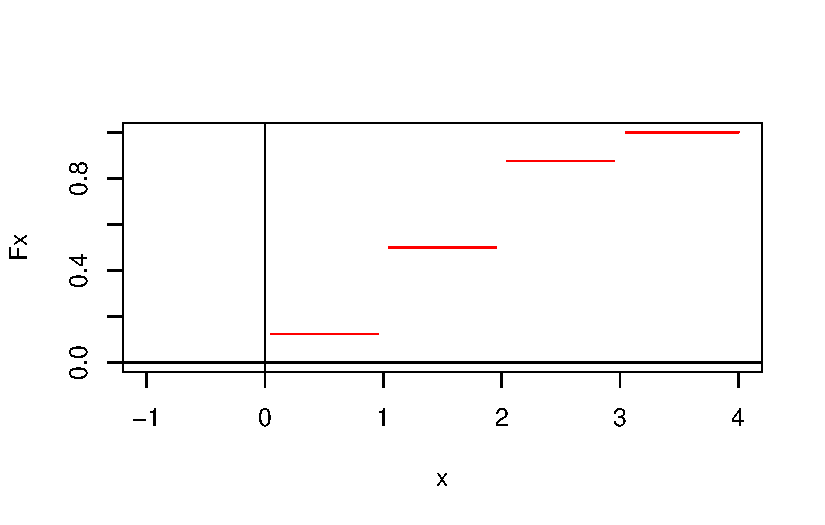
\includegraphics{probabilidad_files/figure-pdf/unnamed-chunk-1-1.pdf}

Por ejemplo, la probabilidad de que se obtenga 0 a 1 aguilas es
\(\frac{1}{8}\).

\end{tcolorbox}

\begin{tcolorbox}[enhanced jigsaw, titlerule=0mm, left=2mm, opacityback=0, toprule=.15mm, colframe=quarto-callout-caution-color-frame, bottomrule=.15mm, breakable, coltitle=black, opacitybacktitle=0.6, bottomtitle=1mm, colback=white, arc=.35mm, leftrule=.75mm, toptitle=1mm, colbacktitle=quarto-callout-caution-color!10!white, title={Ejemplo (\textbf{\emph{Duración de una llamada telefónica}})}, rightrule=.15mm]

Para las variables aleatorias continuas, la froma de la función de
distribución es un poco distinta, pero sigue cumpliendo las mismas
propiedades.

A continuación se representa una función de distribución acumulada de la
variable aleatoria \(X\) que podría ser usada para modelar la duración
de las llamadas telefónicas.

\[ F_X(x)=\begin{cases}0 & \text{ si } x\leq0\\ 1-e^{-x} & \text{ si } 0< x\end{cases} \]

En este caso, se puede ver que la probabilidad de que la variable
aleatoria \(X\) sea menor a cero es 0, ya que el soporte de la
distribución son los números reales positivos.

Como puede apreciarse, conociendo la función de distribución es posible
obtener las probabilidades de cualquier evento, simplemente evaluando
los valores en la función, por ejemplo:

\begin{itemize}
\item
  \(P(X<2)=1-e^{-2}=0.8646\)
\item
  \(P(X>5)=1-(1-e^{-5})=0.0067\)
\item
  \(P(1<X<3)=P(X<3)-P(X<1)=0.3180\)
\end{itemize}

\end{tcolorbox}

\begin{remark}
Se debe tener cuidado cuando se calcula probabilidades de variables
aleatorias discretas ya que en general no es lo mismo \(P(X< x)\) que
\(P(X\leq x)\).
\end{remark}

\subsection{Función de densidad}\label{funciuxf3n-de-densidad}

Otra función relacionada con las variables aleatorias es la función de
densidad.

A diferencia de la función de distribución, esta función es distinta
según si la variable aleatoria es discreta o continua. Primero se
definirá para el caso discreto y posteriormente para el caso continuo.

\subsection{Variables aleatorias
discretas}\label{variables-aleatorias-discretas}

\begin{definition}[Variable aleatoria
discreta]\protect\hypertarget{def-vad}{}\label{def-vad}

Se definirá una variable aleatoria \(X\) como discreta si el rango de
\(X\) es numerable. Si una variable aleatoria \(X\) es discreta,
entonces su función de distribución acumulada correspondiente
\(F_X(\cdot)\) se definirá como discreta.

\end{definition}

\begin{definition}[Función de densidad discreta de una variable
aleatoria discreta]\protect\hypertarget{def-fdd}{}\label{def-fdd}

Si \(X\) es una variable aleatoria discreta con \(D_x=x_1,x_2,\ldots\)
entonces la función, denotada por \(f_X(\cdot)\) y definida por

\[ f_X(x)=\begin{cases}P(X=x_j) & \text{ si } x\in D_x\\ 0 & \text{ cualquier otro caso. }\end{cases} \]

es la función de densidad discreta de \(X\).

\end{definition}

\begin{remark}
En ocasiones se usa la función indicadora \(I_{D_x}(x)=1\) si
\(x\in D_x\) y \(I_{D_x}(x)=0\) si \(x\notin D_x\) para expresar la
función de densidad en una sola línea.
\end{remark}

\begin{theorem}[]\protect\hypertarget{thm-uno}{}\label{thm-uno}

Sea \(X\) una variable aleatoria discreta. \(F_X(\cdot)\) puede ser
obtenido a partir de \(f_X(\cdot)\), y viceversa.

\end{theorem}

\begin{definition}[Función de densidad
discreta]\protect\hypertarget{def-ddf}{}\label{def-ddf}

Cualquier función \(f(\cdot)\) con dominio \(\mathbb R\) y contradominio
\([0,1]\) se define como una \emph{función de densidad discreta} si para
algún conjunto contable \(D=\{x_1, x_2,\ldots\}\) se cumple lo
siguiente;

\begin{enumerate}
\def\labelenumi{\roman{enumi}.}
\item
  \(f(x_j)>0\) para \(j=1,2,\ldots.\)
\item
  \(f(x)=0\) para \(x\neq x_j\) con \(j=1,2,\ldots.\)
\item
  \(\sum_D f(x_j)=1\)
\end{enumerate}

\end{definition}

\subsection{Variables aleatorias
continuas}\label{variables-aleatorias-continuas}

\begin{definition}[Variable aleatoria
continua]\protect\hypertarget{def-vac}{}\label{def-vac}

Se llama variable aleatoria continua a \(X\) si existe una función
\(f_X(\cdot)\) tal que \(F_X(x)=\int_{-\infty}^x f_X(u) du\) para cada
número real \(x\). La función de distribución acumulada \(F_X(\cdot)\)
de una variable aleatoria continua \(X\) se llama \emph{absolutamente
continua.}

\end{definition}

\begin{definition}[Función de densidad de una variable aleatoria
continua]\protect\hypertarget{def-pfdvac}{}\label{def-pfdvac}

Si \(X\) es una variable aleatoria continua, la función \(f_X(\cdot)\)
en \(F_X(x)=\int_{-\infty}^x f_X(u)du\) se llama \emph{función de
densidad} de \(X\).

\end{definition}

\begin{remark}
En ocasiones se usa la función indicadora \(I_{(a,b)}(x)=1\) si
\(x\in (a,b)\) y \(I_{(a,b)}(x)=0\) si \(x\notin (a,b)\) para expresar
la función de densidad en una sola línea.
\end{remark}

\begin{theorem}[]\protect\hypertarget{thm-dos}{}\label{thm-dos}

Si \(X\) es una variable aleatoria continua, entonces \(F_X(\cdot)\) se
puede obtener a partir de una función \(f_X(\cdot)\), y viceversa.

\end{theorem}

Las demostraciones del Teorema~\ref{thm-uno} y Teorema~\ref{thm-dos}
pueden ser consultados en (Mood, Graybill, y Boes 1986).

\begin{tcolorbox}[enhanced jigsaw, titlerule=0mm, left=2mm, opacityback=0, toprule=.15mm, colframe=quarto-callout-caution-color-frame, bottomrule=.15mm, breakable, coltitle=black, opacitybacktitle=0.6, bottomtitle=1mm, colback=white, arc=.35mm, leftrule=.75mm, toptitle=1mm, colbacktitle=quarto-callout-caution-color!10!white, title={Ejemplo (\textbf{\emph{Duración de una llamada telefónica}})}, rightrule=.15mm]

Usando el teorema fundamental del cálculo, se puede probar la propiedad
anterior. Se ilustrará para el ejemplo de la duración de llamadas
telefónicas.

Supóngase que la función de distribución para modelar la duración de las
llamadas telefónicas es

\[ F_X(x)=\begin{cases}0 & \text{ si } x \le 0\\ 1-e^{-x} & \text{ si } 0< x\end{cases} \]

Se observa que \(F_X(x)\) está definida en dos partes, por lo que la
función no es \emph{absolutamente continua} en cero, por lo que solo
será diferenciable en el intervalo de los reales positivos.

\[ f_X(x)=\frac{dF_X(x)}{dx}=\frac{d (1-e^{-x})}{dx}=-\frac{d e^{-x}}{dx}=e^{-x} \]

es decir;

\[ f_X(x)=e^{-x}I_{(0,\infty)}(x). \]

Por otro lado, se observa que

\[ F_X(x)= \int_{\infty}^x e^{-u}du=\int_0^x e^{-u}du=1-e^{-x}, \]

es decir

\[ F_X(x)=1-e^{-x} I_{(0,\infty)}(x) \]

De esta manera, se comprueba la propiedad.

\end{tcolorbox}

\begin{remark}
Se utilizará el término ``función de densidad'' sin el modificador de
``discreta'' o ``de probabilidad'' para representar cualquier tipo de
densidad.
\end{remark}

\section{Vectores aleatorios}\label{vectores-aleatorios}

\begin{definition}[Vector aleatorio
\(n-\)dimensional]\protect\hypertarget{def-randvec}{}\label{def-randvec}

Sean \(X_1,X_2,\cdots, X_n\) variables aleatorias reales definidas sobre
el mismo espacio de probabilidad \((\Omega, \mathfrak F, P)\). La
función \(\mathbf X:\Omega\to\mathbb R^n\) definida como

\[ \mathbf X(\omega)= (X_1(\omega),\cdots,X_n(\omega)) \]

se denomina vector aleatorio \(n-\)dimensional.

\end{definition}

\begin{definition}[Distribución de un vector
aleatorio]\protect\hypertarget{def-drv}{}\label{def-drv}

Sea \(\mathbf X\) un vector aleatorio \(n-\)dimensional. La medida de
probabilidad definida por

\[ P_{\mathbf X} (B) := P(\mathbf X\in B); B\in \mathcal B_n \]

es denominada la distribución del vector aleatorio \(\mathbf X\).

\end{definition}

\begin{definition}[Función de masa de probabilidad
conjunta]\protect\hypertarget{def-dcva}{}\label{def-dcva}

Sea \(\mathbf X= (X_1,X_2,\cdots,X_n)\) un vector aleatorio de \(n\)
dimensiones. Si las variables aleatorias \(X_i\), donde
\(i=1,\cdots,n\), son todas discretas, se afirma que el vector aleatorio
\(\mathbf X\) es discreto. En esta situación, la función de masa de
probabilidad de \(\mathbf X\), también conocida como la \emph{función de
distribución conjunta} de las variables aleatorias
\(X_1, X_2, \cdots, X_n\), queda definida por

\[ p_\mathbf{X}(x):=\begin{cases}P(\mathbf X=x) & \text{ si } x \text{  pertenece a la imagen de } \mathbf X\\ 0 & \text{ en caso contrario. } \end{cases} \]

\end{definition}

\begin{definition}[Función de distribución acumulada
conjunta]\protect\hypertarget{def-FDAC}{}\label{def-FDAC}

Sea \(\mathbf X=(X_1,X_2,\cdots, X_n)\) un vector aleatorio de \(n\)
dimensiones. La función definida por

\[ F(x_1,x_2,\cdots,x_n):= P(X_1\leq x_1, X_2\leq x_2,\cdots, X_n\leq x_n), \]

para todo \((x_1,x_2,\cdots,x_n)\in\mathbb R^n\) recibe el nombre de
función de distribución acumulativa conjunta de las variables aleatorias
\(X_1, X_2, \cdots, X_n\), o simplemente la función de distribución del
vector aleatorio \(n-\)dimensional \(\mathbf X\).

\end{definition}

\chapter{Estadística}\label{estaduxedstica}

La estadística tiene un origen que se remonta a tiempos antiguos, cuando
las civilizaciones antiguas recopilaban y analizaban datos para tomar
decisiones informadas en diversas áreas. Sin embargo, fue en el siglo
XVII cuando los trabajos de pensadores como John Graunt y William Petty
sentaron las bases para los métodos estadísticos modernos. Graunt
realizó estudios sobre la mortalidad y estableció principios de
recopilación de datos, mientras que Petty aplicó el análisis estadístico
a la economía y la demografía.

En la era moderna, con el advenimiento de la computación y la
disponibilidad de grandes volúmenes de datos, la estadística ha cobrado
una importancia aún mayor. Técnicas avanzadas como el análisis de series
de tiempo, la regresión múltiple, el análisis de componentes principales
y el aprendizaje automático han transformado la forma en que abordamos
la predicción de datos. Estas herramientas permiten modelar relaciones
complejas y patrones ocultos en los datos, lo que es crucial para la
toma de decisiones en áreas como el marketing, la medicina, la economía
y la planificación empresarial.

(Mann 2010) presenta dos significados para la palabra ``estadística''.
En el sentido más común, la estadística hace referencia a hechos
numéricos. El segundo significado de estadística se relaciona con el
campo o disciplina de estudio. Bajo esta perspectiva, la estadística se
define de la siguiente manera

\begin{definition}[Estadística]\protect\hypertarget{def-estad}{}\label{def-estad}

Una estadística es una función de variables aleatorias observables, la
cual es en sí misma una variable aleatoria observable y no contiene
ningún parámetro desconocido.

\end{definition}

\section{Datos univariados}\label{datos-univariados}

En esta sección se definirán conceptos básicos de la estádistica
univariada. Se comienza con los siguientes conceptos;

\begin{definition}[Población]\protect\hypertarget{def-pobla}{}\label{def-pobla}

Una \emph{población} consiste en todos los elementos (individuos,
elementos u objetos) cuyas características se están estudiando. La
población que se está estudiando también se denomina \emph{población
objetivo}.

\end{definition}

\begin{definition}[Parámetro]\protect\hypertarget{def-param}{}\label{def-param}

Un \emph{parámetro} es una característica numérica o descriptiva de una
población o probabilidad distribución.

\end{definition}

\subsection{Valor Esperado y momentos}\label{valor-esperado-y-momentos}

Un concepto sumamente útil en problemas que implican variables
aleatorias o distribuciones es el de la esperanza (valor esperado). En
esta subsección, se presentan definiciones y resultados relacionados con
la esperanza.

\begin{definition}[Media]\protect\hypertarget{def-mean}{}\label{def-mean}

Sea \(X\) una variable aleatoria. La \emph{media} de \(X\), denotada
como \(\mu_X\) o \(\mathrm E[X]\), se define de la siguiente manera:

\[ \mathrm E[X]= \sum x_jf_X(x_j) \]

Si \(X\) es discreta con puntos de masa
\(x_1, x_2, \ldots, x_j, \ldots\).

\[ \mathrm E[X]=\int_{-\infty}^\infty x f_X(x)dx \]

Si \(X\) es continua con una función de densidad de probabilidad
\(f_X(x)\).

\[ \mathrm E[X]=\int_0^\infty [1-F_X(x)]dx-\int_{-\infty}^0 F_X(x) dx \]

para cualquier variable aleatoria \(X\).

\end{definition}

\begin{remark}
\(\mathrm E[X]\) representa el centro de gravedad (o centroide) de la
masa unitaria determinada por la función de densidad de \(X\). De esta
manera, la media de \(X\) proporciona una medida de la ubicación central
de los valores de la variable aleatoria \(X\).
\end{remark}

La media de una variable aleatoria \(X\) era una medida de ubicación
central de la densidad de \(X\). La varianza de una variable aleatoria
\(X\) será una medida de la dispersión o propagación de la densidad de
\(X\).

\begin{definition}[Varianza]\protect\hypertarget{def-var}{}\label{def-var}

Sea \(X\) una variable aleatoria, y se define \(\mu_X\) como
\(\mathrm E[X]\), la \emph{varianza} de \(X\), denotada como
\(\sigma_X^2\) o \(\mathrm{Var}[X]\), se define de la siguiente manera

\[ \mathrm{Var}[X]= \sum_j (x_j-\mu_X)^2 f_X(x_j) \]

si \(X\) es discreta con puntos de masa
\(x_1, x_2, \ldots, x_j, \ldots\).

\[ \mathrm{Var}[X]=\int_{-\infty}^\infty (x-\mu_X)^2f_X(x)dx \]

Si \(X\) es continua con una función de densidad de probabilidad
\(f_X(x)\).

\[ \mathrm{Var}[X]=\int_0^\infty 2x[1-F_X(x)+F_X(-x)]dx - \mu_X^2 \]

para una variable aleatoria \(X\) arbitraria.

\end{definition}

Se vio que una media era el centro de gravedad de una densidad; de
manera similar, la varianza representa el momento de inercia de la misma
densidad con respecto a un eje perpendicular que pasa por el centro de
gravedad.

\begin{definition}[Desviación
estándar]\protect\hypertarget{def-SD}{}\label{def-SD}

Si \(X\) es una variable aleatoria, la \emph{desviación estándar} de
\(X\), denotada por \(\sigma_X\), se define como
\(+\sqrt{\mathrm{Var}[X]}\).

\end{definition}

La desviación estándar de una variable aleatoria, al igual que la
varianza, es una medida de la dispersión o propagación de los valores de
la variable aleatoria. En muchas aplicaciones, es preferible a la
varianza como medida, ya que tendrá las mismas unidades de medida que la
propia variable aleatoria.

\subsubsection{Valor esperado de una función de una variable
aleatoria}\label{valor-esperado-de-una-funciuxf3n-de-una-variable-aleatoria}

Se definió la esperanza de una variable aleatoria arbitraria \(X\),
llamada la media de \(X\). En esta subsección, se definirá la esperanza
de una función de una variable aleatoria para variables aleatorias
discretas o continuas

\begin{definition}[Valor
esperado]\protect\hypertarget{def-VE}{}\label{def-VE}

Sea \(X\) una variable aleatoria y \(g(\cdot)\) una función con dominio
y codominio en la recta real. La esperanza o valor esperado de la
función \(g(\cdot)\) de la variable aleatoria \(X\), denotada por
\(\mathrm E[g(X)]\), se define de la siguiente manera:

\[ \mathrm E[g(X)]=\sum_j g(x_j)f_X(x_j) \]

Si \(X\) es discreta con puntos de masa
\(x_1, x_2, \ldots, x_j, \ldots\) (siempre que esta serie sea
absolutamente convergente).

\[ \mathrm E[g(X)]=\int_{-\infty}^\infty g(x)f_X(x)dx \]

Si \(X\) es continua con función de densidad de probabilidad \(f_X(x)\)
(siempre que \(\int_{-\infty}^\infty |g(x)|f_X(x)dx < \infty\)).

\end{definition}

\begin{remark}
Si \(g(x)=x\), entonces \(\mathrm E[g(X)]=\mathrm E[X]\) es la media de
\(X\). Si \(g(x)=(x-\mu_X)^2\), entonces
\(\mathrm E[g(X)]=\mathrm E[(X-\mu_X)^2]=\mathrm{Var}[X]\).
\end{remark}

\begin{theorem}[]\protect\hypertarget{thm-propve}{}\label{thm-propve}

A continuación se presentan las propiedades del valor esperado:

\begin{enumerate}
\def\labelenumi{\roman{enumi}.}
\item
  \(\mathrm E[c]=c\) para una constante \(c\).
\item
  \(\mathrm E[cg(X)]=c\mathrm E[g(X)]\) para una constante \(c\).
\item
  \(\mathrm E[c_1 g_1(X)+c_2 g_2(X)]=c_1\mathrm E[g_1(X)]+c_2\mathrm E[g_2(X)]\).
\item
  \(\mathrm E[g_1(X)]\leq \mathrm E[g_2(X)]\) si \(g_1(x)\leq g_2(x)\)
  para todo \(x\).
\end{enumerate}

\end{theorem}

\begin{theorem}[]\protect\hypertarget{thm-var}{}\label{thm-var}

Si \(X\) es una variable aleatoria, entonces

\[\mathrm{Var}[X] = \mathrm E[(X-\mathrm E[X])^2] = \mathrm E[X^2] - (\mathrm E[X])^2,\]
siempre que \(\mathrm E[X^2]\) exista.

\end{theorem}

Las pruebas de los teoremas anteriores se pueden consultar en (Mood,
Graybill, y Boes 1986).

\subsubsection{Momentos}\label{momentos}

Los momentos de una variable aleatoria o de una distribución son los
valores esperados de las potencias de la variable aleatoria que tiene la
distribución dada.

\begin{definition}[Momento]\protect\hypertarget{def-moment}{}\label{def-moment}

Si \(X\) es una variable aleatoria, el \(r-\)ésimo momento de \(X\),
generalmente denotado por \(\mu_r'\), se define como

\[ \mu_r'=\mathrm E[X^r] \] si el valor esperado existe.

\end{definition}

Note que \(\mu_1' = \mathrm E[X] = \mu_X\), que es la media de \(X\).

\begin{definition}[Cuantil]\protect\hypertarget{def-quant}{}\label{def-quant}

El \(q-\)ésimo cuantil de una variable aleatoria \(X\) o de su
distribución correspondiente se denota como \(\xi_q\) y se define como
el número más pequeño \(\xi\) que cumple con la condición
\(F_X(\xi) \geq q\).

\end{definition}

Si \(X\) es una variable aleatoria continua, entonces el \(q-\)ésimo
cuantil de \(X\) se calcula como el número más pequeño \(\xi\) que
cumple con la condición \(F_X(\xi) = q\).

\begin{definition}[Mediana]\protect\hypertarget{def-median}{}\label{def-median}

La mediana de una variable aleatoria \(X\), denotada como
\(\mathrm{med}_X\)\emph{,} \(\mathrm{med}(x)\) \emph{o} \(\xi_{0.5}\),
es el quinto cuantil.

\end{definition}

\subsection{Muestreo}\label{muestreo}

\begin{definition}[Muestra]\protect\hypertarget{def-muestra}{}\label{def-muestra}

Una porción de la población seleccionada para el estudio es conocida
como una \emph{muestra}.

\end{definition}

Una muestra puede ser aleatoria o no aleatoria. En una muestra
aleatoria, cada elemento de la población tiene la posibilidad de ser
incluido en la muestra. Sin embargo, en una muestra no aleatoria este
puede no ser el caso.

\begin{definition}[Muestra
aleatoria]\protect\hypertarget{def-mas}{}\label{def-mas}

Sean \(X_1, X_2, \ldots, X_n\) variables aleatorias con una densidad
conjunta \(f_{(X_1,\ldots, X_n)}(\cdot,\ldots, \cdot)\) que se
descompone de la siguiente manera:

\[f_{X_1,X_2,\ldots, X_n}(x_1,x_2,\ldots,x_n)=f(x_1)f(x_2)\cdots f(x_n),\]
donde \(f(\cdot)\) es la densidad (común) de cada \(X_i\). Entonces, se
define que \(X_1, X_2, \ldots, X_n\) es una \emph{muestra aleatoria} de
tamaño \(n\) de una población con densidad \(f(\cdot)\).

\end{definition}

\begin{definition}[Media
Muestral]\protect\hypertarget{def-medmues}{}\label{def-medmues}

El primer momento de la muestra es la \emph{media muestral}, definida
como

\[ \bar{X}= \bar{X_n}=\frac{1}{n}\sum_{i=1}^n X_i, \]

donde \(X_1, X_2, \ldots, X_n\) es una muestra aleatoria de una densidad
\(f(\cdot)\). \(\bar{X}\) es una función de las variables aleatorias
\(X_1, \ldots, X_n\), y por lo tanto, en teoría se puede determinar la
distribución de \(\bar{X}\).

\end{definition}

\begin{definition}[Varianza
muestral]\protect\hypertarget{def-varmues}{}\label{def-varmues}

Sea \(X_1, X_2, \ldots, X_n\) una muestra aleatoria con densidad
\(f(\cdot)\), entonces

\[ S_n^2=S^2=\frac{1}{n-1}\sum_{i=1}^n (X_i-\bar{X})^2\qquad \text{para  } n>1 \]

se define como la \emph{varianza muestral}.

\end{definition}

\begin{theorem}[]\protect\hypertarget{thm-meanvar}{}\label{thm-meanvar}

Sea \(X_1, X_2, \ldots, X_n\) una muestra aleatoria con densidad
\(f(\cdot)\), la cual tiene una media \(\mu\) y una varianza finita
\(\sigma^2\), y sea \(\bar{X} = \frac{1}{n}\sum\limits_{i=1}^n X_i\).
Luego,

\[ \mathrm{E}[\bar X]=\mu_{\bar X}=\mu\qquad \text{ y }\qquad \mathrm{Var}[\bar X]=\sigma_{\bar X}^2 =\frac{1}{n}\sigma^2.\]

\end{theorem}

\begin{theorem}[Teorema del límite
central]\protect\hypertarget{thm-TCL}{}\label{thm-TCL}

Supongamos que \(f(\cdot)\) es una densidad con media \(\mu\) y varianza
finita \(\sigma^2\). Si \(\bar{X}_n\) es el promedio de una muestra
aleatoria de tamaño \(n\) extraída de \(f(\cdot)\) y definimos la
variable aleatoria \(Z_n\) como

\[ Z_n = \frac{\bar{X_n}-\mathrm E[\bar X_n]}{\sqrt{\mathrm{Var}[\bar X_n]}}=\frac{\bar X_n-\mu}{\sigma/\sqrt n} \]
Entonces, la distribución de \(Z_n\) se acerca a la distribución normal
estándar a medida que \(n\) tiende a infinito.

\end{theorem}

\section{Datos multivariados}\label{datos-multivariados}

Cuando dos o más variables aleatorias son observadas en miembros de una
muestra aleatoria, los datos resultantes se denominan datos
multivariados. El caso especial de dos variables se refiere como datos
bivariados.

\begin{tcolorbox}[enhanced jigsaw, titlerule=0mm, left=2mm, opacityback=0, toprule=.15mm, colframe=quarto-callout-caution-color-frame, bottomrule=.15mm, breakable, coltitle=black, opacitybacktitle=0.6, bottomtitle=1mm, colback=white, arc=.35mm, leftrule=.75mm, toptitle=1mm, colbacktitle=quarto-callout-caution-color!10!white, title={Ejemplo}, rightrule=.15mm]

Considere los datos en la Tabla~\ref{tbl-cal} que representan una
muestra de 30 estudiantes en una universidad grande que fueron asignados
al azar a un curso de Introducción a la Informática. En la Tabla se
muestran las puntuaciones del cuestionario, además de la calificación
del examen final de cada estudiante.

\begin{longtable}[]{@{}
  >{\raggedright\arraybackslash}p{(\columnwidth - 16\tabcolsep) * \real{0.0789}}
  >{\raggedright\arraybackslash}p{(\columnwidth - 16\tabcolsep) * \real{0.1579}}
  >{\raggedright\arraybackslash}p{(\columnwidth - 16\tabcolsep) * \real{0.0921}}
  >{\raggedright\arraybackslash}p{(\columnwidth - 16\tabcolsep) * \real{0.0789}}
  >{\raggedright\arraybackslash}p{(\columnwidth - 16\tabcolsep) * \real{0.1579}}
  >{\raggedright\arraybackslash}p{(\columnwidth - 16\tabcolsep) * \real{0.0921}}
  >{\raggedright\arraybackslash}p{(\columnwidth - 16\tabcolsep) * \real{0.0789}}
  >{\raggedright\arraybackslash}p{(\columnwidth - 16\tabcolsep) * \real{0.1579}}
  >{\raggedright\arraybackslash}p{(\columnwidth - 16\tabcolsep) * \real{0.1053}}@{}}
\caption{Puntuaciones y calificación
final.}\label{tbl-cal}\tabularnewline
\toprule\noalign{}
\begin{minipage}[b]{\linewidth}\raggedright
Est.
\end{minipage} & \begin{minipage}[b]{\linewidth}\raggedright
Puntuación
\end{minipage} & \begin{minipage}[b]{\linewidth}\raggedright
Final
\end{minipage} & \begin{minipage}[b]{\linewidth}\raggedright
Est.
\end{minipage} & \begin{minipage}[b]{\linewidth}\raggedright
Puntuación
\end{minipage} & \begin{minipage}[b]{\linewidth}\raggedright
Final
\end{minipage} & \begin{minipage}[b]{\linewidth}\raggedright
Est.
\end{minipage} & \begin{minipage}[b]{\linewidth}\raggedright
Puntuación
\end{minipage} & \begin{minipage}[b]{\linewidth}\raggedright
Final
\end{minipage} \\
\midrule\noalign{}
\endfirsthead
\toprule\noalign{}
\begin{minipage}[b]{\linewidth}\raggedright
Est.
\end{minipage} & \begin{minipage}[b]{\linewidth}\raggedright
Puntuación
\end{minipage} & \begin{minipage}[b]{\linewidth}\raggedright
Final
\end{minipage} & \begin{minipage}[b]{\linewidth}\raggedright
Est.
\end{minipage} & \begin{minipage}[b]{\linewidth}\raggedright
Puntuación
\end{minipage} & \begin{minipage}[b]{\linewidth}\raggedright
Final
\end{minipage} & \begin{minipage}[b]{\linewidth}\raggedright
Est.
\end{minipage} & \begin{minipage}[b]{\linewidth}\raggedright
Puntuación
\end{minipage} & \begin{minipage}[b]{\linewidth}\raggedright
Final
\end{minipage} \\
\midrule\noalign{}
\endhead
\bottomrule\noalign{}
\endlastfoot
1 & 7.4 & 79.8 & 11 & 7.6 & 80.7 & 21 & 8.0 & 84.2 \\
2 & 8.4 & 82.0 & 12 & 8.8 & 94.5 & 22 & 9.0 & 87.8 \\
3 & 8.8 & 76.1 & 13 & 6.1 & 50.1 & 23 & 8.9 & 94.1 \\
4 & 6.4 & 62.7 & 14 & 7.2 & 68.3 & 24 & 7.5 & 78.2 \\
5 & 10.0 & 98.2 & 15 & 6.6 & 64.4 & 25 & 5.5 & 62.4 \\
6 & 5.5 & 43.0 & 16 & 7.0 & 67.2 & 26 & 8.5 & 85.1 \\
7 & 7.3 & 76.5 & 17 & 5.3 & 53.9 & 27 & 7.4 & 77.8 \\
8 & 5.9 & 61.4 & 18 & 7.9 & 78.8 & 28 & 6.3 & 67.6 \\
9 & 7.1 & 78.5 & 19 & 8.1 & 85.7 & 29 & 7.7 & 70.2 \\
10 & 7.9 & 88.7 & 20 & 7.6 & 81.7 & 30 & 6.9 & 73.6 \\
& & & & & & Suma & 222.6 & 2253.2 \\
\end{longtable}

Los valores medios y las desviaciones estándar se proporcionan a
continuación. Las puntuaciones del cuestionario están en el vector \(x\)
y las puntuaciones del examen final están en \(y\). Se tienen los
siguientes resultados:

\begin{verbatim}
Media(x) = 7.42
\end{verbatim}

\begin{verbatim}
Desviación estándar(x) = 1.15
\end{verbatim}

\begin{verbatim}
Media(y) = 75.11
\end{verbatim}

\begin{verbatim}
Desviación estándar(y) = 13.15
\end{verbatim}

Los histogramas de estas dos variables se muestran en la
Figura~\ref{fig-histo}. Allí se puede observar que los histogramas de
ambas variables tienen una forma aproximadamente en campana, con las
puntuaciones del examen final ligeramente sesgadas hacia la izquierda.
Al examinar el histograma en la Figura~\ref{fig-histo}(b), se observa
que la media de las puntuaciones del examen final parece ser de
alrededor de 75, lo cual es coherente con los resultados anteriores. La
mayoría de las puntuaciones están entre 60 y 90, con algunas por encima
de 90 y algunas por debajo de 60.

\begin{figure}[H]

\centering{

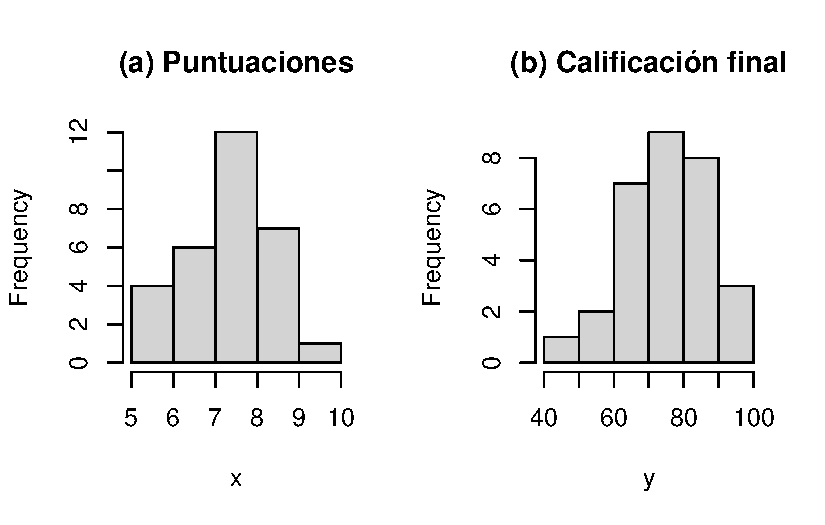
\includegraphics{estadistica_files/figure-pdf/unnamed-chunk-2-1.pdf}

}

\caption{\label{fig-histo}Puntajes y calificaciones finales para una
muestra aleatoria de 30 estudiantes inscritos al curso.}

\end{figure}%

\end{tcolorbox}

Los histogramas, las medias y las desviaciones estándar no proporcionan
información sobre cómo dos variables están relacionadas entre sí. Como
ejemplo, un instructor probablemente quisiera saber si los estudiantes
que les fue bien en el cuestionario también tendieron a desempeñarse
bien en el examen final, y viceversa. También podría querer saber si
algunos estudiantes que les fue mal en el cuestionario mejoraron
drásticamente su calificación en el examen final. Los histogramas y las
estadísticas de muestra mostrados anteriormente no responden a estas
preguntas.

Lo que se necesita son medidas de la relación entre las dos variables.
Los parámetros poblacionales más comunes utilizados para medir tales
relaciones son la covarianza, \(\gamma_{XY}\), y la correlación,
\(\rho_{XY}\).

\begin{definition}[Covarianza]\protect\hypertarget{def-cov}{}\label{def-cov}

Si \(X\) e \(Y\) son dos variables aleatorias definidas en el mismo
espacio de probabilidad, la \emph{covarianza} de \(X\) e \(Y\), denotada
como \(\mathrm{Cov}[X,Y]\) o \(\gamma_{XY}\), se define como
\[\gamma_{XY}=\mathrm{Cov}[X,Y]=\mathrm E[(X-\mu_X)(Y-\mu_Y)]\] siempre
que la esperanza indicada exista.

\end{definition}

\begin{definition}[Correlación]\protect\hypertarget{def-corr}{}\label{def-corr}

La \emph{correlación}, denotada como \(\rho[X,Y]\) o \(\rho_{XY}\), de
las variables aleatorias \(X\) e \(Y\), se define como

\[ \rho_{XY}=\frac{\gamma_{XY}}{\sigma_X \sigma_Y} \]

siempre que \(\gamma_{XY}, \sigma_X\) y \(\sigma_Y\) existan, con
\(\sigma_X, \sigma_Y>0\).

\end{definition}

Técnicamente, la covarianza es el valor esperado (o promedio teórico)
del producto cruzado \((X-\mu_X)(Y-\mu_Y)\). Es una medida de cómo dos
variables ``se mueven juntas''. Para facilitar la interpretación,
generalmente utilizamos la correlación, que es una versión
``estandarizada'' de la covarianza que tiene la propiedad
\(-1 \leq \rho_{XY}\leq 1\) para cualquier par de variables aleatorias
\(X\) e \(Y\).

\begin{remark}
\leavevmode

\begin{enumerate}
\def\labelenumi{\alph{enumi}.}
\item
  \(\gamma_{XX}=\mathrm E[(X-\mu_X)(X-\mu_X)]=\mathrm E[(X-\mu_X)^2]=\sigma_X^2\).
\item
  \(\rho_{XX}=\frac{\sigma_X^2}{\sigma_X \sigma_X}=1\).
\end{enumerate}

\end{remark}

\begin{corollary}[]\protect\hypertarget{cor-covind}{}\label{cor-covind}

Si \(X\) e \(Y\) son independientes, entonces \(\gamma_{XY}=0\).

\begin{proof}
Observe que

\[ \begin{split}\mathrm{Cov}[X,Y]=\mathrm E[(X-\mu_X)(Y-\mu_Y)]=\mathrm E[X-\mu_X]\mathrm E[Y-\mu_Y]=0\end{split} \]

Ya que \(\mathrm E[(X-\mu_X)]=0\).
\end{proof}

\end{corollary}

\begin{definition}[Variables aleatorias no
correlacionadas]\protect\hypertarget{def-uncorr}{}\label{def-uncorr}

Las variables aleatorias \(X\) e \(Y\) se definen como no
correlacionadas si y solo si \(\mathrm{Cov}[X,Y]=0\).

\end{definition}

\begin{remark}
La afirmación contraria al corolario anterior no siempre es cierta; es
decir, \(\mathrm{Cov}[X,Y]=0\) no siempre implica que \(X\) e \(Y\) sean
independientes.
\end{remark}

\chapter{Procesos estocásticos}\label{procesos-estocuxe1sticos}

Los procesos estocásticos desempeñan un papel fundamental en la
modelización y análisis de una amplia gama de fenómenos en diversas
disciplinas, desde la física hasta la economía. Estos procesos son
esenciales para comprender y predecir el comportamiento de sistemas que
involucran aleatoriedad y variabilidad en el tiempo.

Un proceso estocástico (o probabilístico) puede considerarse una
generalización de una muestra aleatoria, en el sentido de que las
variables aleatorias \textbf{no son necesariamente independientes} y su
distrbución podría cambiar. (Castañeda, Arunachalam, y Dharmaraja 2014)
proporciona la siguiente definición para proceso estocástico.

\begin{definition}[Proceso
estocástico]\protect\hypertarget{def-PE}{}\label{def-PE}

Un \emph{proceso estocástico} real es una colección de variables
aleatorias \(\{X_t; t\in T\}\) definida en un espacio de probabilidad
común \((\Omega, \mathfrak{F}, P)\) con valores en \(\mathbb{R}\). \(T\)
se le llama al conjunto índice del proceso o espacio paramétrico, que
generalmente es un subconjunto de \(\mathbb R\). El conjunto de valores
que la variable aleatoria \(X_t\) puede tomar se denomina \emph{espacio
de estado del proceso} y es denotado por \(S\).

\end{definition}

De la definición anterior se entiende que las variables
\emph{dependerán} del parámetro \(t\) (usualmente el tiempo) y están
ordenadas. Además el conjunto \(T\) puede ser discreto o continuo. Si el
conjunto de índices \(T\) es discreto, se le conoce como~\emph{proceso
estocástico de tiempo discreto}~mientras que si \(T\) es continuo, se le
conoce como~\emph{proceso estocástico de tiempo coninuo}. Las variables
aleatorias \(X_t\) pueden tomar tanto valores continuos o valores
discretos. Note que si se fija un punto \(t\), se tiene \(X_t\) una
variable aleatoria (Ross 1995).

\begin{definition}[Trayectoria]\protect\hypertarget{def-realiza}{}\label{def-realiza}

La asignación definida para cada \(\omega\in\Omega\) fijo,
\[\begin{split}X(\omega): & T\to S\\ &t\mapsto X_t(\omega)\end{split}\]
se denomina una trayectoria de muestra del proceso a lo largo del tiempo
o una realización del proceso estocástico.

\end{definition}

\begin{definition}[Proceso completamente
específicado]\protect\hypertarget{def-pcesp}{}\label{def-pcesp}

Se dice que un proceso estocástico \(\{X(t):t\in T\}\) está
completamente especificado si para cualquier valor del tiempo
\(t_1<t_2<\cdots<t_n\) con \(n\in\mathbb N\), la distribución conjunta
de \((X_{t_1}, X_{t_2},\cdots,X_{t_n})\) es conocida.

\end{definition}

\begin{definition}[Proceso estocástico con incrementos
independientes]\protect\hypertarget{def-incind}{}\label{def-incind}

Si, para todo \(t_0,t_1,t_2,\ldots,t_n\) tal que
\(t_0<t_1<t_2<\cdots<t_n\), las variables aleatorias
\(X_{t_0}, X_{t_1}-X_{t_0}, X_{t_2}-X_{t_1},\ldots,X_{t_n}-X_{t_{n-1}}\)
son independientes (o de manera equivalente, \(X_{t+\tau}-X_\tau\) es
independiente de \(X_s\) para \(s< \tau\)), entonces se dice que el
proceso \(\{X_t; t\in T\}\) es un \emph{proceso con incrementos
independientes.}

\end{definition}

\begin{definition}[Proceso estocástico con incrementos
estacionarios]\protect\hypertarget{def-incest}{}\label{def-incest}

Se dice que un proceso estocástico \({X_t; t\in T}\) tiene
\emph{incrementos estacionarios} si \(X_{t_2+\tau}-X_{t_1+\tau}\) tiene
la misma distribución que \(X_{t_2}-X_{t_1}\) para todas las elecciones
de \(t_1,t_2\) y \(\tau>0\).

\end{definition}

\part{Series de tiempo}

\chapter{Series de Tiempo}\label{series-de-tiempo-1}

Las series de tiempo tienen su origen en la necesidad de comprender y
predecir patrones en datos secuenciales a lo largo del tiempo. Desde
tiempos antiguos, las civilizaciones han registrado observaciones
cronológicas para prever fenómenos naturales, eventos económicos y otros
procesos cambiantes.

Sin embargo, el enfoque más sistemático en el análisis de series de
tiempo comenzó a tomar forma en el campo de la estadística y la
econometría en el siglo XX. Pioneros como Norbert Wiener y Andrey
Kolmogorov sentaron las bases teóricas alrededor de los procesos
estocásticos y las cadenas de Markov, que son fundamentales para modelar
la evolución temporal de variables.

La importancia de las series de tiempo en la predicción de datos radica
en su capacidad para capturar patrones temporales y tendencias en
conjuntos de datos. A medida que acumulamos datos a lo largo del tiempo,
podemos identificar relaciones y ciclos que permiten realizar
pronósticos futuros. Esto es especialmente valioso en campos como la
economía, la meteorología, la epidemiología y las finanzas, donde
comprender los patrones temporales es esencial para tomar decisiones
informadas.

En la actualidad, con el advenimiento de la computación y las técnicas
de análisis más sofisticadas, las series de tiempo han cobrado aún más
importancia. Los modelos matemáticos y estadísticos avanzados, como los
modelos ARIMA (AutoRegressive Integrated Moving Average) y las redes
neuronales recurrentes, permiten analizar y predecir series de tiempo
con mayor precisión y complejidad. Estos modelos son fundamentales para
la toma de decisiones estratégicas en una variedad de industrias, ya que
ayudan a anticipar tendencias, identificar patrones estacionales y
enfrentar la incertidumbre en el futuro.

Una serie de tiempo es una secuencia de mediciones que describen la
evolución de un fenómeno o variable a lo largo del tiempo; es una
secuencia cronológicamente ordenada de valores de medición sobre el
estado de una variable cuantitativa de un fenómeno o proceso. Dichas
mediciones están ordenadas respecto al tiempo y son generalmente
dependientes entre sí, (Woodward, Sadler, y Robertson 2022).

En términos generales, se puede considerar una serie de tiempo como una
colección de observaciones realizadas de forma secuencial en el tiempo.
El interés de este capítulo no estará en las series que son
deterministas, sino en aquellas cuyos valores se comportan de acuerdo
con las leyes de la probabilidad, se discutirán los fundamentos
involucrados en el análisis estadístico de series de tiempo. Para
empezar, se debe tener más cuidado con la definición de serie temporal,
pues en realidad, una serie de tiempo es un tipo especial de proceso
estocástico.

\begin{definition}[Serie de
tiempo]\protect\hypertarget{def-ts}{}\label{def-ts}

Un proceso estocástico \(X(t); t\in T\) se define como una colección de
variables aleatorias, donde \(T\) es un conjunto de índices para el cual
todas las variables aleatorias, \(X(t)\), donde \(t\) pertenece a \(T\),
están definidas en el mismo espacio muestral. Cuando \(T\) representa el
tiempo, se hace referencia al proceso estocástico como una \emph{serie
de tiempo}.

\end{definition}

Si \(T\) toma un rango continuo de valores (por ejemplo,
\(T=(-\infty,\infty)\) o \(T=(0,\infty)\)) , el proceso se dice que es
un \emph{proceso de parámetro continuo}. Si, por otro lado, \(T\) toma
un conjunto discreto de valores (por ejemplo, \(T = \{0, 1, 2,\ldots\}\)
o \(T = \{0, \pm 1, \pm 2,\ldots \}\)), el proceso se dice que es un
\emph{proceso de parámetro discreto}. De hecho, es común referirse a
estos como procesos continuos y discretos, respectivamente.

Se utilizará la notación de subíndice, \(X_t\), cuando se esté tratando
específicamente con un proceso de parámetro discreto. Sin embargo,
cuando el proceso involucrado sea de parámetro continuo o de tipo no
especificado, se utilizará la notación de función, \(X(t)\). Además,
cuando no haya confusión, a menudo se utiliza la notación \(\{X(t)\}\) o
simplemente \(X(t)\) para denotar una serie de tiempo. De manera
similar, a menudo se acortará \(\{X_t;t=0,\pm 1,\ldots \}\) a
\(X_t,t=0,\pm 1,\ldots\) o simplemente se usará \(X_t\).

Recordemos que una variable aleatoria, \(\gamma\) , es una función
definida en un espacio muestral \(\Omega\) cuyo rango son los números
reales. Un valor observado de la variable aleatoria \(\gamma\) es un
número real \(y=\gamma(\omega)\) para algún \(\omega\in\Omega\). Para
una serie de tiempo \(\{X(t)\}\), su ``valor''
\(\{X(t,\omega);t\in T\}\) para algún \(\omega\in\Omega\) fijo es una
colección de números reales. Esto lleva a la siguiente definición.

\begin{definition}[Realización]\protect\hypertarget{def-realizacion}{}\label{def-realizacion}

Una \emph{realización} de la serie de tiempo \(\{X(t);t\in T\}\) es el
conjunto de resultados de valores reales, \(\{X(t,\omega);t\in T\}\)
para un valor fijo de \(\omega \in \Omega\).

\end{definition}

La colección de todas las posibles realizaciones se denomina
\emph{conjunto}, y, para un valor dado de \(t\), la expectativa de la
variable aleatoria \(X(t)\) se denomina \emph{media del conjunto} y se
denotará como \(\mathrm E[X(t)]=\mu(t)\) . La varianza de \(X(t)\) se
expresa como \(\mathrm{Var}[X(t)]=\mathrm E[(X(t)-\mu(t))^2]\) y a
menudo se denota como \(\sigma^2(t)\) ya que también puede depender de
\(t\).

\phantomsection\label{.remark}
De especial interés en el análisis de una serie temporal es la
covarianza entre \(X(t_1)\) y \(X(t_2)\), donde \(t_1, t_2\in T\). Dado
que esta es la covarianza (Definición~\ref{def-cov}) dentro de la misma
serie temporal, se refiere a ella como \emph{autocovarianza}. De igual
manera, se refiere a correlación (Definición~\ref{def-corr}) como
\emph{autocorrelación} y se denotan por
\(\gamma(t_1,t_2)= \mathrm{E}[(X(t_1)-\mu(t_1))(X(t_2)-\mu(t_2))]\) y
\(\rho(t_1,t_2)=\frac{\gamma(t_1,t_2)}{\sigma(t_1)\sigma(t_2)}\)
respectivamente.

\section{Series de tiempo
estacionarias}\label{series-de-tiempo-estacionarias}

En el estudio de una serie de tiempo, es común que solo se tenga
disponible una única realización de la serie. El análisis de una serie
temporal basado únicamente en una realización es análogo a analizar las
propiedades de una variable aleatoria en función de una sola
observación. Los conceptos de estacionariedad y ergodicidad jugarán un
papel importante en mejorar la capacidad de análisis de una serie
temporal basada en una única realización de manera efectiva. Un proceso
se considera estacionario si está en un estado de ``equilibrio
estadístico''. El comportamiento básico de dicha serie de tiempo no
cambia con el tiempo. Como ejemplo, para dicho proceso, \(\mu(t)\) no
dependería del tiempo y, por lo tanto, podría ser denotado como \(\mu\)
para todo \(t\). Parecería que, dado que \(x(t)\) para cada \(t\in T\)
proporciona información sobre la media del conjunto, \(\mu\), podría ser
posible estimar \(\mu\) en función de una única realización. Un proceso
ergódico es aquel para el cual promedios de conjunto como \(\mu\) pueden
estimarse consistentemente a partir de una sola realización. En esta
sección, se presentarán definiciones más formales de estacionariedad. La
noción más restrictiva de estacionariedad es la de estacionariedad
estricta, que se define de la siguiente manera.

\begin{definition}[Proceso estrictamente
estacionario]\protect\hypertarget{def-PPE}{}\label{def-PPE}

Se dice que un proceso \(\{X(t); t \in T\}\) es estrictamente
estacionario si para cualquier \(t_1, t_2,\ldots, t_k \in T\) y
cualquier \(h \in T\), la distribución conjunta de
\(\{X(t_1), X(t_2),\ldots , X(t_k)\}\) es idéntica a la de
\(\{X(t_1 + h), X(t_2 + h),\ldots, X(t_k + h)\}\).

\end{definition}

La estacionariedad estricta requiere, entre otras cosas, que para
cualquier \(t_1, t_2 \in T\), las distribuciones de \(X(t_1)\) y
\(X(t_2)\) deben ser las mismas, y además que todas las distribuciones
bivariadas de pares \(\{X(t), X(t + h)\}\) sean iguales para todos los
\(h\), etc. El requisito de estacionariedad estricta es riguroso y suele
ser difícil de establecer matemáticamente. De hecho, para la mayoría de
las aplicaciones, las distribuciones involucradas no se conocen. Por
esta razón, se han desarrollado nociones menos restrictivas de
estacionariedad. La más común de ellas es la estacionariedad por
covarianza.

\begin{definition}[Estacionariedad por
covarianza]\protect\hypertarget{def-estcov}{}\label{def-estcov}

La serie de tiempo \(\{X(t); t \in T\}\) se considera estacionaria por
covarianza si

\begin{enumerate}
\def\labelenumi{\arabic{enumi}.}
\item
  \(\mathrm E[X(t)] = \mu\) (constante para todo \(t\))
\item
  \(\mathrm{Var}[X(t)] = \sigma^2 < \infty\) (es decir, una constante
  finita para todo \(t\))
\item
  \(\gamma (t_1, t_2)\) depende solo de \(t_2 − t_1\).
\end{enumerate}

\end{definition}

\begin{remark}
La estacionariedad por covarianza también se conoce como estacionariedad
débil, estacionariedad en el sentido amplio y estacionariedad de segundo
orden. En el resto de esta tesis, a menos que se especifique lo
contrario, el término estacionariedad se referirá a la estacionariedad
por covarianza.
\end{remark}

En las series de tiempo, al igual que en la mayoría de las otras áreas
de la estadística, los datos no correlacionados desempeñan un papel
importante. No hay dificultad en definir dicho proceso en el caso de una
serie temporal de parámetro discreto. Es decir, la serie temporal
\(\{X_t; t = 0, \pm 1, \pm 2,\ldots\}\) se llama ``proceso puramente
aleatorio'' si los \(X_t\) son variables aleatorias no correlacionadas.
Al considerar procesos puramente aleatorios, solo nos interesará el caso
en el que los \(X_t\) también estén distribuidos de manera idéntica. En
esta situación, es más común referirse a la serie de tiempo como ruido
blanco. La siguiente definición resume estas observaciones.

\begin{definition}[Ruido blanco
discreto]\protect\hypertarget{def-ruidob}{}\label{def-ruidob}

Una serie de tiempo se llama ruido blanco discreto si:

\begin{enumerate}
\def\labelenumi{\arabic{enumi}.}
\item
  Los \(X_t\) están distribuidos de manera idéntica.
\item
  \(\gamma (t_1, t_2) = 0\) cuando \(t_2 \ne t_1\).
\item
  \(\gamma (t, t) = \sigma^2\), donde \(0 < \sigma^2 < \infty\) .
\end{enumerate}

\end{definition}

\subsection{Funciones de autocovarianza y autocorrelación para series
temporales
estacionarias}\label{funciones-de-autocovarianza-y-autocorrelaciuxf3n-para-series-temporales-estacionarias}

Si una serie temporal es estacionaria por covarianza, entonces la
función de autocovarianza \(\gamma (t, t + h)\) depende únicamente de
\(h\). Por lo tanto, para procesos estacionarios, se denota esta función
de autocovarianza como \(\gamma(h)\). De manera similar, la función de
autocorrelación para un proceso estacionario se define como

\begin{equation}\phantomsection\label{eq-autocorrelacion}{
\rho(h):=\gamma(h)/\sigma^2.
}\end{equation}

En coherencia con la notación anterior, al tratar con una serie temporal
de parámetro discreto, se utiliza la notación subíndice \(\gamma_h\) y
\(\rho_h\).

La función de autocovarianza de una serie de tiempo estacionaria
satisface las siguientes propiedades:

\begin{enumerate}
\def\labelenumi{\roman{enumi}.}
\item
  \(\gamma(0)=\sigma^2\).
\item
  \(|\gamma(h)|\leq \gamma(0)\) para todo \(h\).
\item
  \(\gamma(h)=\gamma(-h)\).
\item
  La función \(\gamma(h)\) es semidefinida positiva. Esto es, para
  cualquier conjunto de puntos de tiempo \(t_1, t_2,\ldots,t_k\in T\) y
  para los reales \(b_1,b_2,\ldots, b_k\), se tiene

  \[\sum_{i=1}^k \sum_{j=1}^k \gamma(t_i-t_j)b_i b_j\geq 0.
  \]
\end{enumerate}

La función de autocorrelación satisface las siguientes propiedades
análogas:

\begin{enumerate}
\def\labelenumi{\roman{enumi}.}
\item
  \(\rho (0) = 1\).
\item
  \(|\rho (h)|\leq 1\) para todo \(h\).
\item
  \(\rho(h)=\rho(-h)\).
\item
  La función \(\rho (h)\) es semidefinida positiva, y para series de
  tiempo discretas definidas en \(t = 0, \pm 1, \pm 2,\ldots\), la
  matriz

  \[
  \boldsymbol{\rho}_k = \begin{pmatrix}1 & \rho_1 & \ldots & \rho_k\\
  \rho_1 & 1 & \ldots & \rho_{k-1}\\
  \vdots & \vdots & \ddots & \vdots\\
  \rho_k & \rho_{k+1}&\ldots & 1\end{pmatrix}
  \]

  es semidefinida positiva para cada \(k\).
\end{enumerate}

\subsection{Estimación de la media, autocovarianza y autocorrelación
para series de tiempo
estacionarias.}\label{estimaciuxf3n-de-la-media-autocovarianza-y-autocorrelaciuxf3n-para-series-de-tiempo-estacionarias.}

Como se ha comentado anteriormente, un objetivo común en el análisis de
series temporales es el de obtener información relativa a una serie
temporal sobre la base de una única realización. En esta sección,
discutimos la estimación de μ, γ (h) y ρ(h) a partir de una sola
realización. Nuestro enfoque serán series temporales de parámetros
discretos donde T = \{\ldots{} , −2, −1, 0, 1, 2, \ldots\}, en cuyo caso
se observa típicamente una realización de longitud finita t = 1, 2,
\ldots{} ,n.~Los resultados análogos a los que se dan aquí están
disponibles para series temporales de parámetros continuos, pero sólo se
mencionarán brevemente en ejemplos. Se remite al lector a Parzen (1962)
para los resultados más generales.

\section{Holt-Winters}\label{holt-winters}

El enfoque Holt-Winters es una técnica desarrollada por los economistas
Holt (Holt 1957) y Winters (Winters 1960).

Este método de predicción es una extensión del suavizado exponencial y
se aplica a series temporales univariadas. El método no necesita un gran
almacenamiento de datos y es simple. Es adecuado para la predicción a
corto plazo y utiliza la función de máxima verosimilitud para estimar
los parámetros. Existen dos modelos de Holt-Winter que utilizan modelos
aditivos o multiplicativos basados en el componente estacional. Los
modelos aditivos se aplican para un modelo con una tendencia lineal y
con una tendencia exponencial. El modelo aditivo de Holt-Winters para
datos con tendencia y estacionalidad que no aumentan con el tiempo es
adecuado. Matemáticamente, el modelo aditivo se expresa de la siguiente
manera:

\[ \hat{y}_{t+\frac{h}{t}}= a_t+h\cdot b_t+s_{t-p+1+(h-1)mod(p),} \]

donde \(a_t, b_t\) y \(s_t\) se expresan de la siguiente manera:

\[ \begin{split}a_t &= \alpha(y_t-s_{t-p})+(1-\alpha)(a_{t-1}+b_{t-1})\\ b_t &= \beta(a_t-a_{t-1})+(1-\beta)b_{t-1}\\ s_t &= \gamma(y_t-a_t)+(1-\gamma)s_{t-p}.\end{split} \]

La función multiplicativa de predicción de Holt-Winters se expresa de la
siguiente manera:

\[ \hat{y}_{t+\frac{h}{t}}= (a_t+h\cdot b_t)\cdot s_{t-p+1+(h-1)mod(p),} \]

donde \(a_t, b_t\) y \(s_t\) se expresan de la siguiente manera:

\[ \begin{split}a_t &= \alpha(y_t/s_{t-p})+(1-\alpha)(a_{t-1}+b_{t-1})\\ b_t &= \beta(a_t-a_{t-1})+(1-\beta)b_{t-1}\\ s_t &= \gamma(y_t/a_t)+(1-\gamma)s_{t-p}.\end{split} \]

donde \(a_t, b_t\) y \(s_t\), se indican el nivel, la pendiente y la
estacionalidad de las series temporales en el tiempo \(t>0\),
respectivamente. La notación \(p\) indicaba el número de estaciones en
un año. Además, los coeficientes \(0\leq \alpha,\beta, \gamma \leq 1\).
Finalmente, \(h> 0\) es el horizonte de pronóstico.

\part{Redes Neuronales}

Las redes neuronales tienen sus raíces en la búsqueda de emular el
funcionamiento del cerebro humano en la década de 1940. McCulloch y
Pitts (1943) propusieron el concepto inicial de una ``neurona
artificial'' que podría realizar operaciones lógicas básicas. Sin
embargo, fue en la década de 1950 cuando el psicólogo Frank Rosenblatt
desarrolló el ``perceptrón'', Rosenblatt (1960), un tipo de red neuronal
que podía aprender a reconocer patrones a través de entrenamiento.

A pesar de su potencial, las limitaciones del perceptrón y la falta de
avances en la capacidad computacional llevaron a un declive en la
investigación en redes neuronales en los años siguientes. Sin embargo,
en la década de 1980 y 1990, hubo un resurgimiento del interés debido a
nuevos algoritmos de aprendizaje y avances en el hardware, permitiendo
el entrenamiento de redes más complejas.

La importancia de las redes neuronales en la predicción de datos radica
en su capacidad para aprender patrones y relaciones en conjuntos de
datos vastos y complejos. A través del proceso de entrenamiento, una red
neuronal ajusta sus pesos y conexiones internas para capturar
características relevantes en los datos. Esto les permite realizar
tareas como clasificación y regresión, lo que a su vez permite la
predicción de resultados futuros.

Con el tiempo, las redes neuronales se han vuelto más sofisticadas,
dando lugar a arquitecturas como las redes neuronales convolucionales
(CNN) para el procesamiento de imágenes y las redes neuronales
recurrentes (RNN) para el procesamiento de secuencias. Además, el
surgimiento del aprendizaje profundo (deep learning) ha permitido el
entrenamiento de redes neuronales con muchas capas, lo que ha mejorado
significativamente su capacidad para abordar problemas complejos de
predicción.

\section*{MLP}\label{mlp}
\addcontentsline{toc}{section}{MLP}

\markright{MLP}

MLP se introdujo por primera vez a finales de la década de 1950 y
principios de la de 1960 Joseph (1961) como una forma de entrenar a las
computadoras para realizar tareas de reconocimiento de patrones.

El perceptrón multicapa (MLP) es un tipo de red neuronal artificial que
se utiliza ampliamente para diversas tareas de aprendizaje automático,
como la clasificación y la regresión. Se llama perceptrón de múltiples
capas porque tiene muchas capas de nodos (conocidos como neuronas
artificiales) que se conectan entre sí.

La arquitectura de red se muestra en la Figura~\ref{fig-estmlp}. Los MLP
incluyen al menos tres capas. Este modelo consta de entradas,
ponderaciones, sesgos y una función de activación que produce la salida.
Cada entrada \(x_i\) a una neurona, \(j\) se multiplica por un
coeficiente adaptativo \(w_{ij}\), llamado peso, luego con una función
de activación no lineal \((\varphi)\) como sigmoide, tangente
hiperbólica, etc. La suma ponderada de las entradas se obtiene como se
muestra en la siguiente ecuación:

\[ o_i = \varphi\left(\sum_{j=1}^d (x_jw_{ij}+b_j)\right) \]

Una función de activación permite a la red asignar una entrada a una
salida, y también la red aprende a representar datos complejos. En otras
palabras, desde un punto de vista estadístico, los MLP ejecutan una
regresión no lineal.

En la salida \(o_i\) de una neurona en la red MLP, \(d\) es el número de
las entradas \(x_j, b_j\) y \(w_{ij}\) son los sesgos y pesos asociados
con cada \(x_j\). En la fase de entrenamiento del modelo, los
coeficientes o ponderaciones de la red se ajustan en función del cálculo
de la función de error y en los siguientes pasos, las ponderaciones se
actualizan en función de la tasa de aprendizaje y el error en cada
iteración. En el paso final, todos los pasos se repiten hasta alcanzar
el número de épocas.

\begin{figure}

\centering{

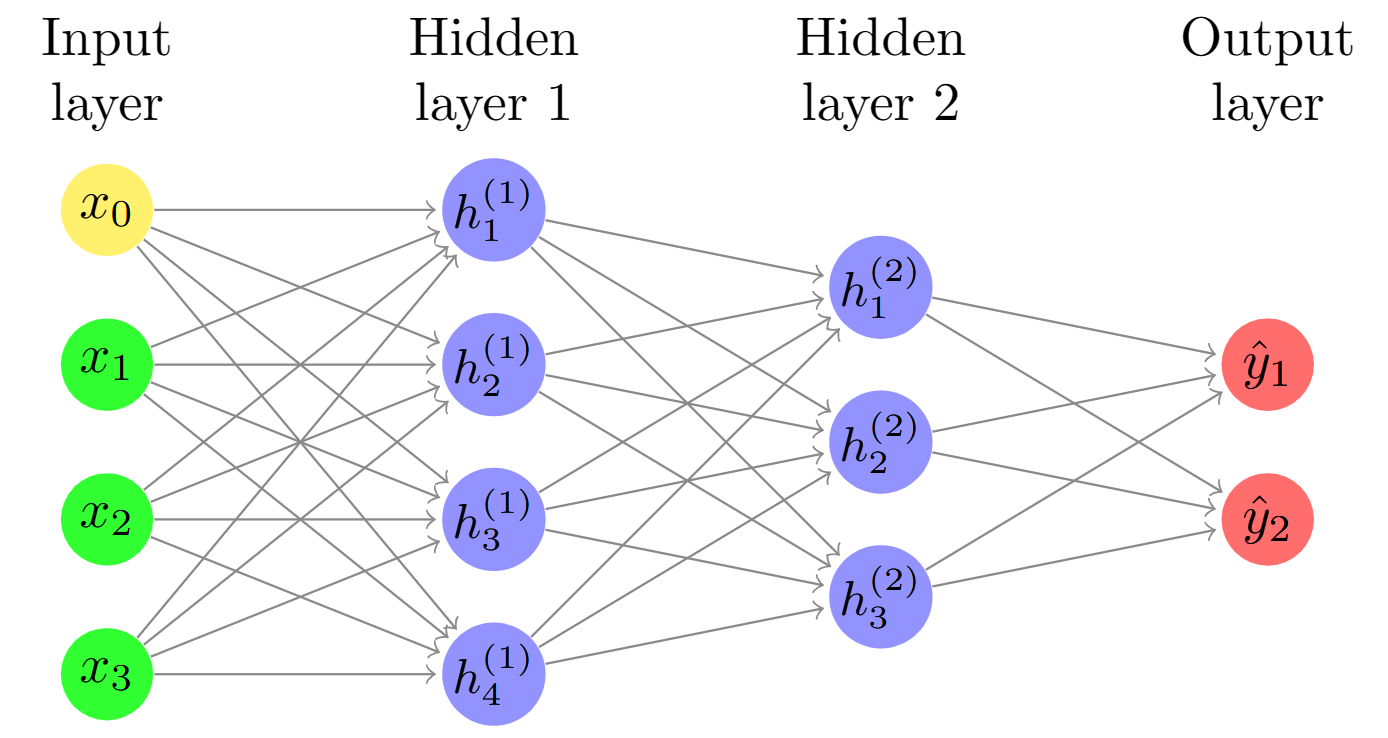
\includegraphics{Cap.png}

}

\caption{\label{fig-estmlp}Estructura de la red MLP}

\end{figure}%

\subsection*{}\label{section}
\addcontentsline{toc}{subsection}{}

\part{Estudio de caso}

A finales de diciembre de 2019, se identificó la aparición de un virus
innovador en Wuhan, China, el cual manifestó un impacto agudo en el
sistema respiratorio y presentó una rápida propagación. La Organización
Mundial de la Salud (OMS) catalogó este virus como el SARS-CoV-2,
perteneciente a la familia de los coronavirus. Aunque algunas
investigaciones y evidencias sugieren que los murciélagos podrían ser el
origen principal del COVID-19, esta afirmación aún no está
definitivamente confirmada y requiere una mayor investigación. Esta
enfermedad infecciosa aguda se caracteriza por su alta tasa de contagio,
lo que llevó a declararla una pandemia global debido a su rápida
expansión y diseminación a nivel mundial.

Los síntomas comunes de esta enfermedad incluyen complicaciones
respiratorias, tos seca, fiebre, escalofríos, dificultad para respirar,
dolor torácico, neumonía, entre otros. No obstante, a medida que
progresa la enfermedad, los síntomas en los pacientes evolucionan y
varían.

Una de las principales problemáticas asociadas a este virus es su
periodo de incubación de hasta 14 días, durante el cual puede
transmitirse la infección sin presentar síntomas. Además, algunas
personas infectadas con el COVID-19 manifiestan síntomas leves,
similares a un resfriado común o a la gripe. Esta pandemia ha ejercido
una presión significativa sobre los gobiernos y los sistemas de salud
pública. La escasez de equipamiento médico en hospitales, incluyendo
camas, unidades de cuidados intensivos, personal médico, ventiladores,
entre otros, constituye uno de los principales desafíos. Asimismo, han
surgido repercusiones económicas y sociales a raíz de la propagación de
la enfermedad y la implementación de cuarentenas estrictas, lo que ha
afectado la salud mental de las comunidades, entre otros aspectos.

\begin{center}
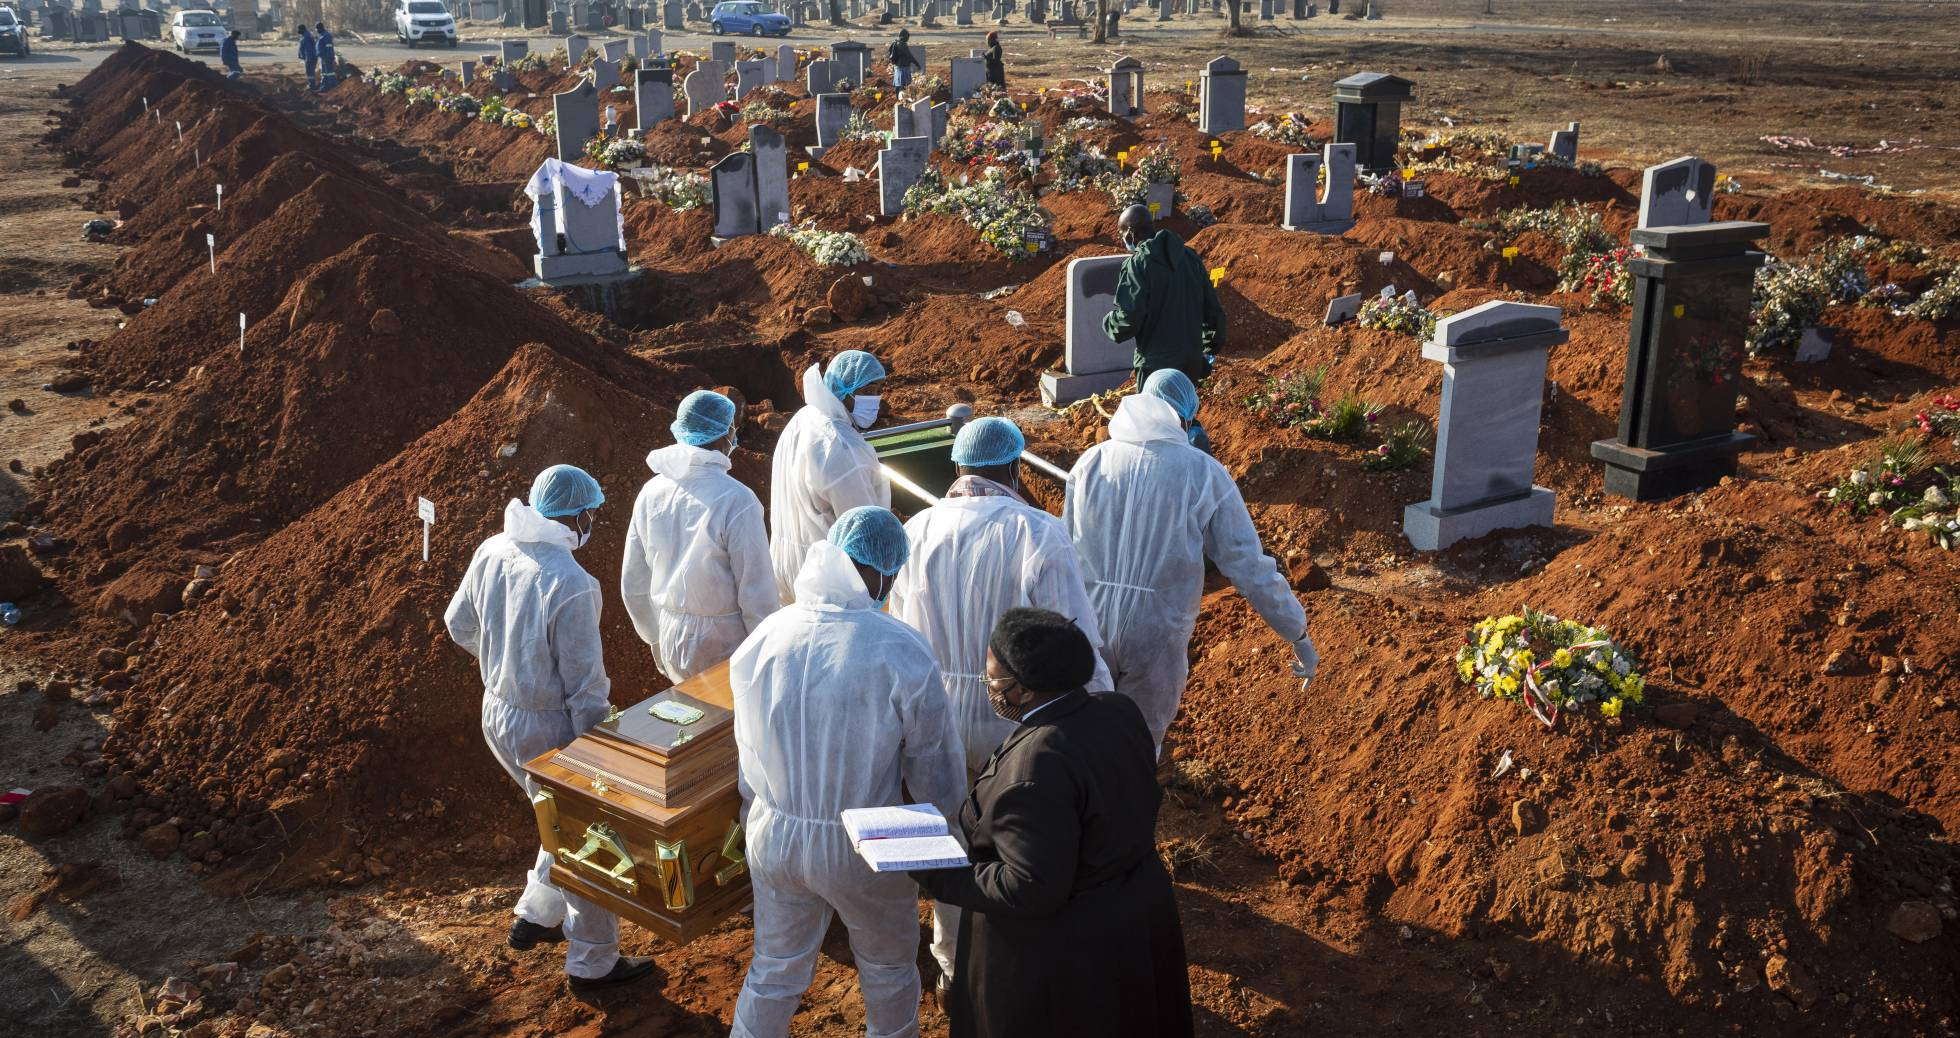
\includegraphics{COVID.jpg}
\end{center}

El surgimiento de las problemáticas mencionadas, sumado a la ausencia de
tratamientos definitivos para esta enfermedad, la naturaleza dinámica
del virus y su propagación global, subraya la necesidad de investigar
exhaustivamente este virus y su comportamiento. Se han explorado
diversos campos y metodologías de pronóstico y modelización. Uno de
estos enfoques de pronóstico radica en la creación de modelos para
anticipar el número de casos futuros, basados en registros de casos
confirmados. Aunque las proyecciones sobre el número de pacientes
futuros no son totalmente precisas, sirven de apoyo a los gobiernos y a
los responsables de políticas de salud para adoptar decisiones cruciales
y aplicar restricciones que reduzcan la prevalencia. Asimismo, resulta
crucial anticipar futuros brotes, posibles mutaciones del virus y su
propagación, especialmente identificar el pico para mitigar sus efectos
graves. Estas proyecciones asisten a los tomadores de decisiones para
prevenir e incluso controlar la propagación de la enfermedad mediante
políticas efectivas y rigurosas. Cabe destacar que la falta de
información suficiente con anticipación constituye uno de los desafíos
principales en el pronóstico, aunque sigue siendo una herramienta de
orientación efectiva para los gobiernos en la contención de la
enfermedad.

Por consiguiente, dado el papel potencialmente efectivo de los modelos
estadísticos y matemáticos en la predicción de la tendencia futura de la
enfermedad, en este estudio se emplearon dos modelos, Holt-Winter y MLP
(Multilayer Perceptron), con el propósito de determinar el mejor modelo
para pronosticar, de manera independiente, el número de casos
confirmados y muertes en Irán para los próximos 30 días.

En el presente estudio, se utilizó el conjunto de datos disponible en el
sitio web \url{https://www.who.int/,} el cual contempla el número
absoluto de casos confirmados y muertes por día, excluyendo otros
factores debido a su falta de disponibilidad.

\chapter{Pronóstico de casos confirmados de COVID-19 en
Irán}\label{pronuxf3stico-de-casos-confirmados-de-covid-19-en-iruxe1n}

\section{Obtención de datos}\label{obtenciuxf3n-de-datos}

Conforme se ha referido previamente, se emplea el conjunto de datos
global informado diariamente, disponible para su descarga en
\url{https://covid19.who.int/WHO-COVID-19-global-data.csv.} Resulta
relevante destacar que la base de datos consultada corresponde al 16 de
Enero del 2023, restringiéndose a los datos concernientes exclusivamente
a los casos confirmados en Irán entre el 20 de febrero y el 15 de agosto
de 2020.

El análisis posterior se ha llevado a cabo empleando el software R
versión 4.3.2. Con el propósito de realizar el análisis de los datos y
la generación de gráficos, se procedió a convertir los datos al formato
\emph{ts}, lo que permitió su representación como una serie temporal.

\begin{Shaded}
\begin{Highlighting}[]
\CommentTok{\# Se crea un objeto \textquotesingle{}Date\textquotesingle{} diario}
\NormalTok{inds }\OtherTok{\textless{}{-}} \FunctionTok{seq}\NormalTok{(}\FunctionTok{as.Date}\NormalTok{(}\StringTok{"2020{-}02{-}20"}\NormalTok{), }\FunctionTok{as.Date}\NormalTok{(}\StringTok{"2020{-}08{-}15"}\NormalTok{), }\AttributeTok{by =} \StringTok{"day"}\NormalTok{)}
\CommentTok{\# Se crea un objeto \textquotesingle{}serie de tiempo\textquotesingle{} de frecuencia diaria}
\NormalTok{Confirmed\_ts }\OtherTok{\textless{}{-}} \FunctionTok{ts}\NormalTok{(Confirmed\_df[}\DecValTok{2}\NormalTok{], }
                   \AttributeTok{start =} \FunctionTok{c}\NormalTok{(}\DecValTok{2020}\NormalTok{, }\FunctionTok{as.numeric}\NormalTok{(}\FunctionTok{format}\NormalTok{(inds[}\DecValTok{1}\NormalTok{], }\StringTok{"\%j"}\NormalTok{))),}
                   \AttributeTok{frequency =} \DecValTok{365}\NormalTok{)}
\end{Highlighting}
\end{Shaded}

\begin{figure}

\centering{

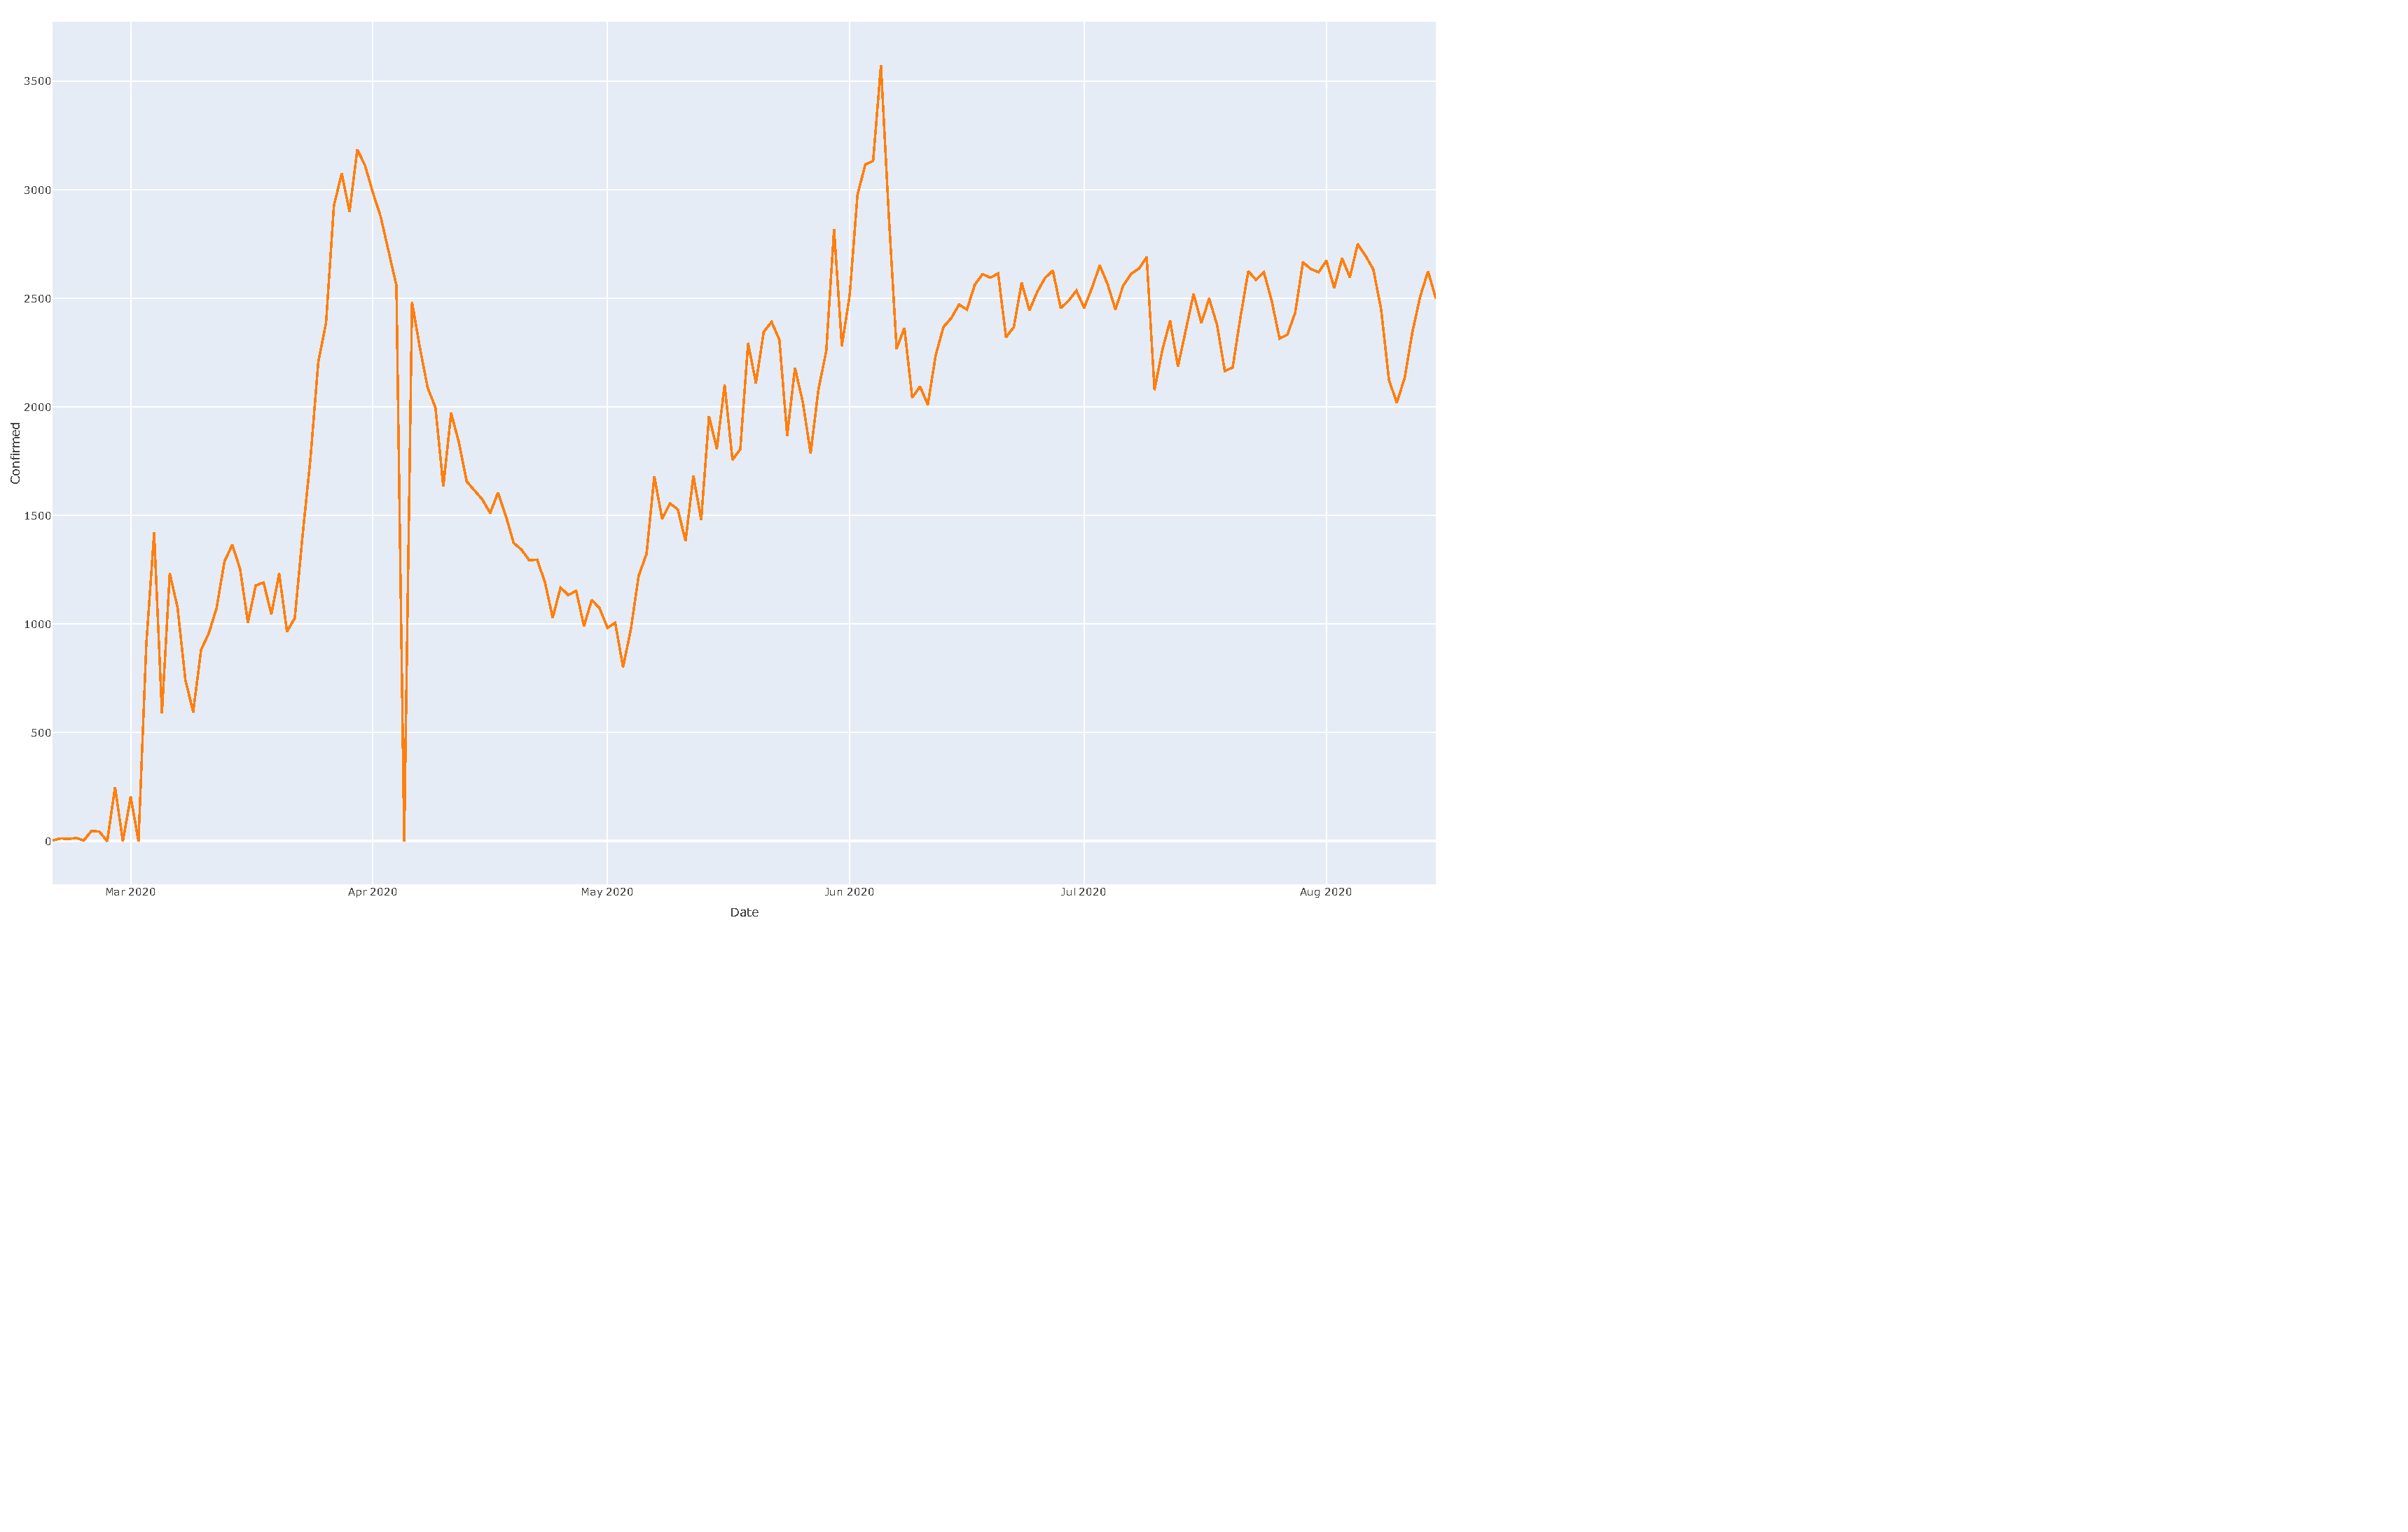
\includegraphics{confirmados_files/figure-pdf/unnamed-chunk-4-1.pdf}

}

\caption{\label{fig-ori}Serie de tiempo de los casos de COVID-19
confirmados en Irán del 20-02-2020 al 15-08-2020}

\end{figure}%

La gráfica de la Figura~\ref{fig-ori} exhibe la serie temporal derivada
de la base de datos, en la cual se evidencia la ausencia de información
para los días 27 y 29 de Febrero, así como para el 02 de Marzo y el 05
de Abril de 2020. Para subsanar esta carencia de datos, se llevó a cabo
una interpolación promedio a fin de sustituir los valores faltantes. La
Tabla~\ref{tbl-datatable} muestra la base de datos con las
modificaciones efectuadas, así como la serie de tiempo
(Figura~\ref{fig-ts}) resultante de estas correcciones.

\begin{table}

\caption{\label{tbl-datatable}Casos confirmados ajustados del 20-02-2020
al 15-08-2020}

\centering{


\includegraphics{confirmados_files/figure-pdf/tbl-datatable-1.pdf}

}

\end{table}%

\begin{figure}

\centering{

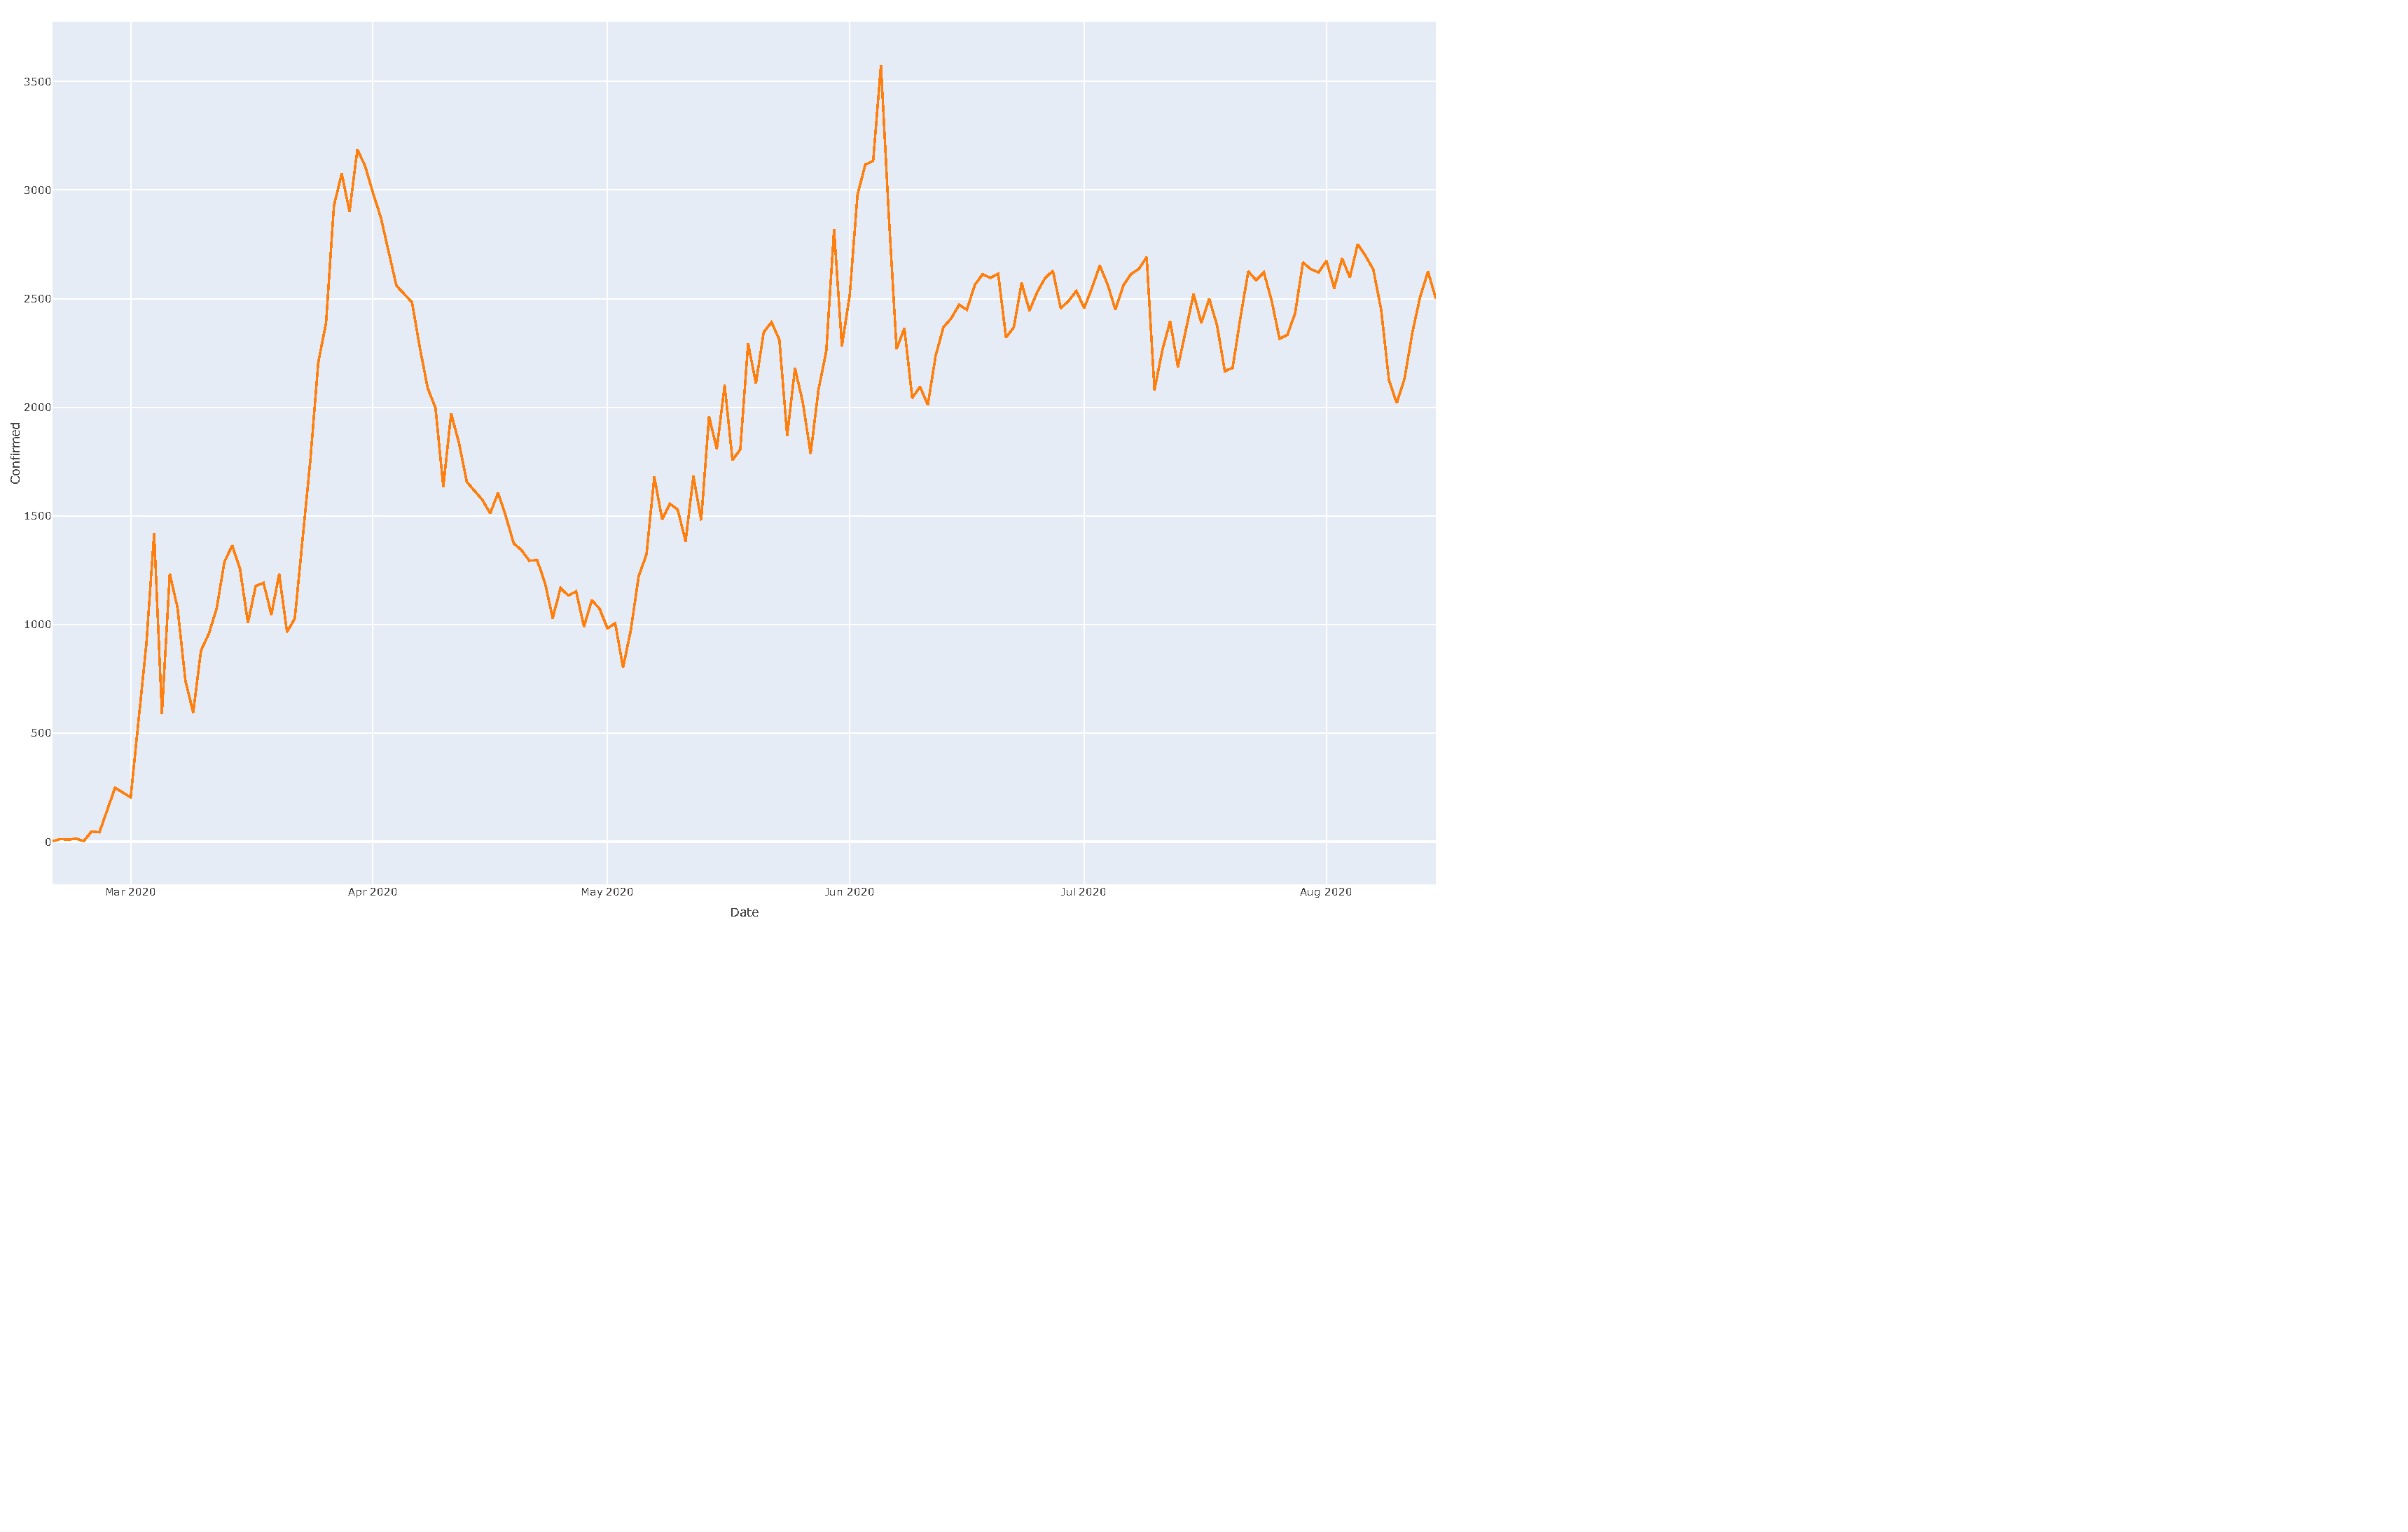
\includegraphics{confirmados_files/figure-pdf/unnamed-chunk-7-1.pdf}

}

\caption{\label{fig-ts}Serie de tiempo de los casos de COVID-19
confirmados en Irán del 20-02-2020 al 15-08-2020}

\end{figure}%

\section{Análisis de la serie de tiempo de casos confirmados de COVID-19
en
Irán}\label{anuxe1lisis-de-la-serie-de-tiempo-de-casos-confirmados-de-covid-19-en-iruxe1n}

\subsection{Estadística descriptiva}\label{estaduxedstica-descriptiva}

Con el propósito de llevar a cabo un análisis exhaustivo de la base de
datos, se ejecuta un estudio de estadística descriptiva que arroja los
resultados correspondientes, incluyendo un gráfico Boxplot
(Figura~\ref{fig-box}) para representar la información obtenida.

\begin{verbatim}
   Min. 1st Qu.  Median    Mean 3rd Qu.    Max. 
      3    1304    2181    1923    2529    3574 
\end{verbatim}

\begin{figure}

\centering{

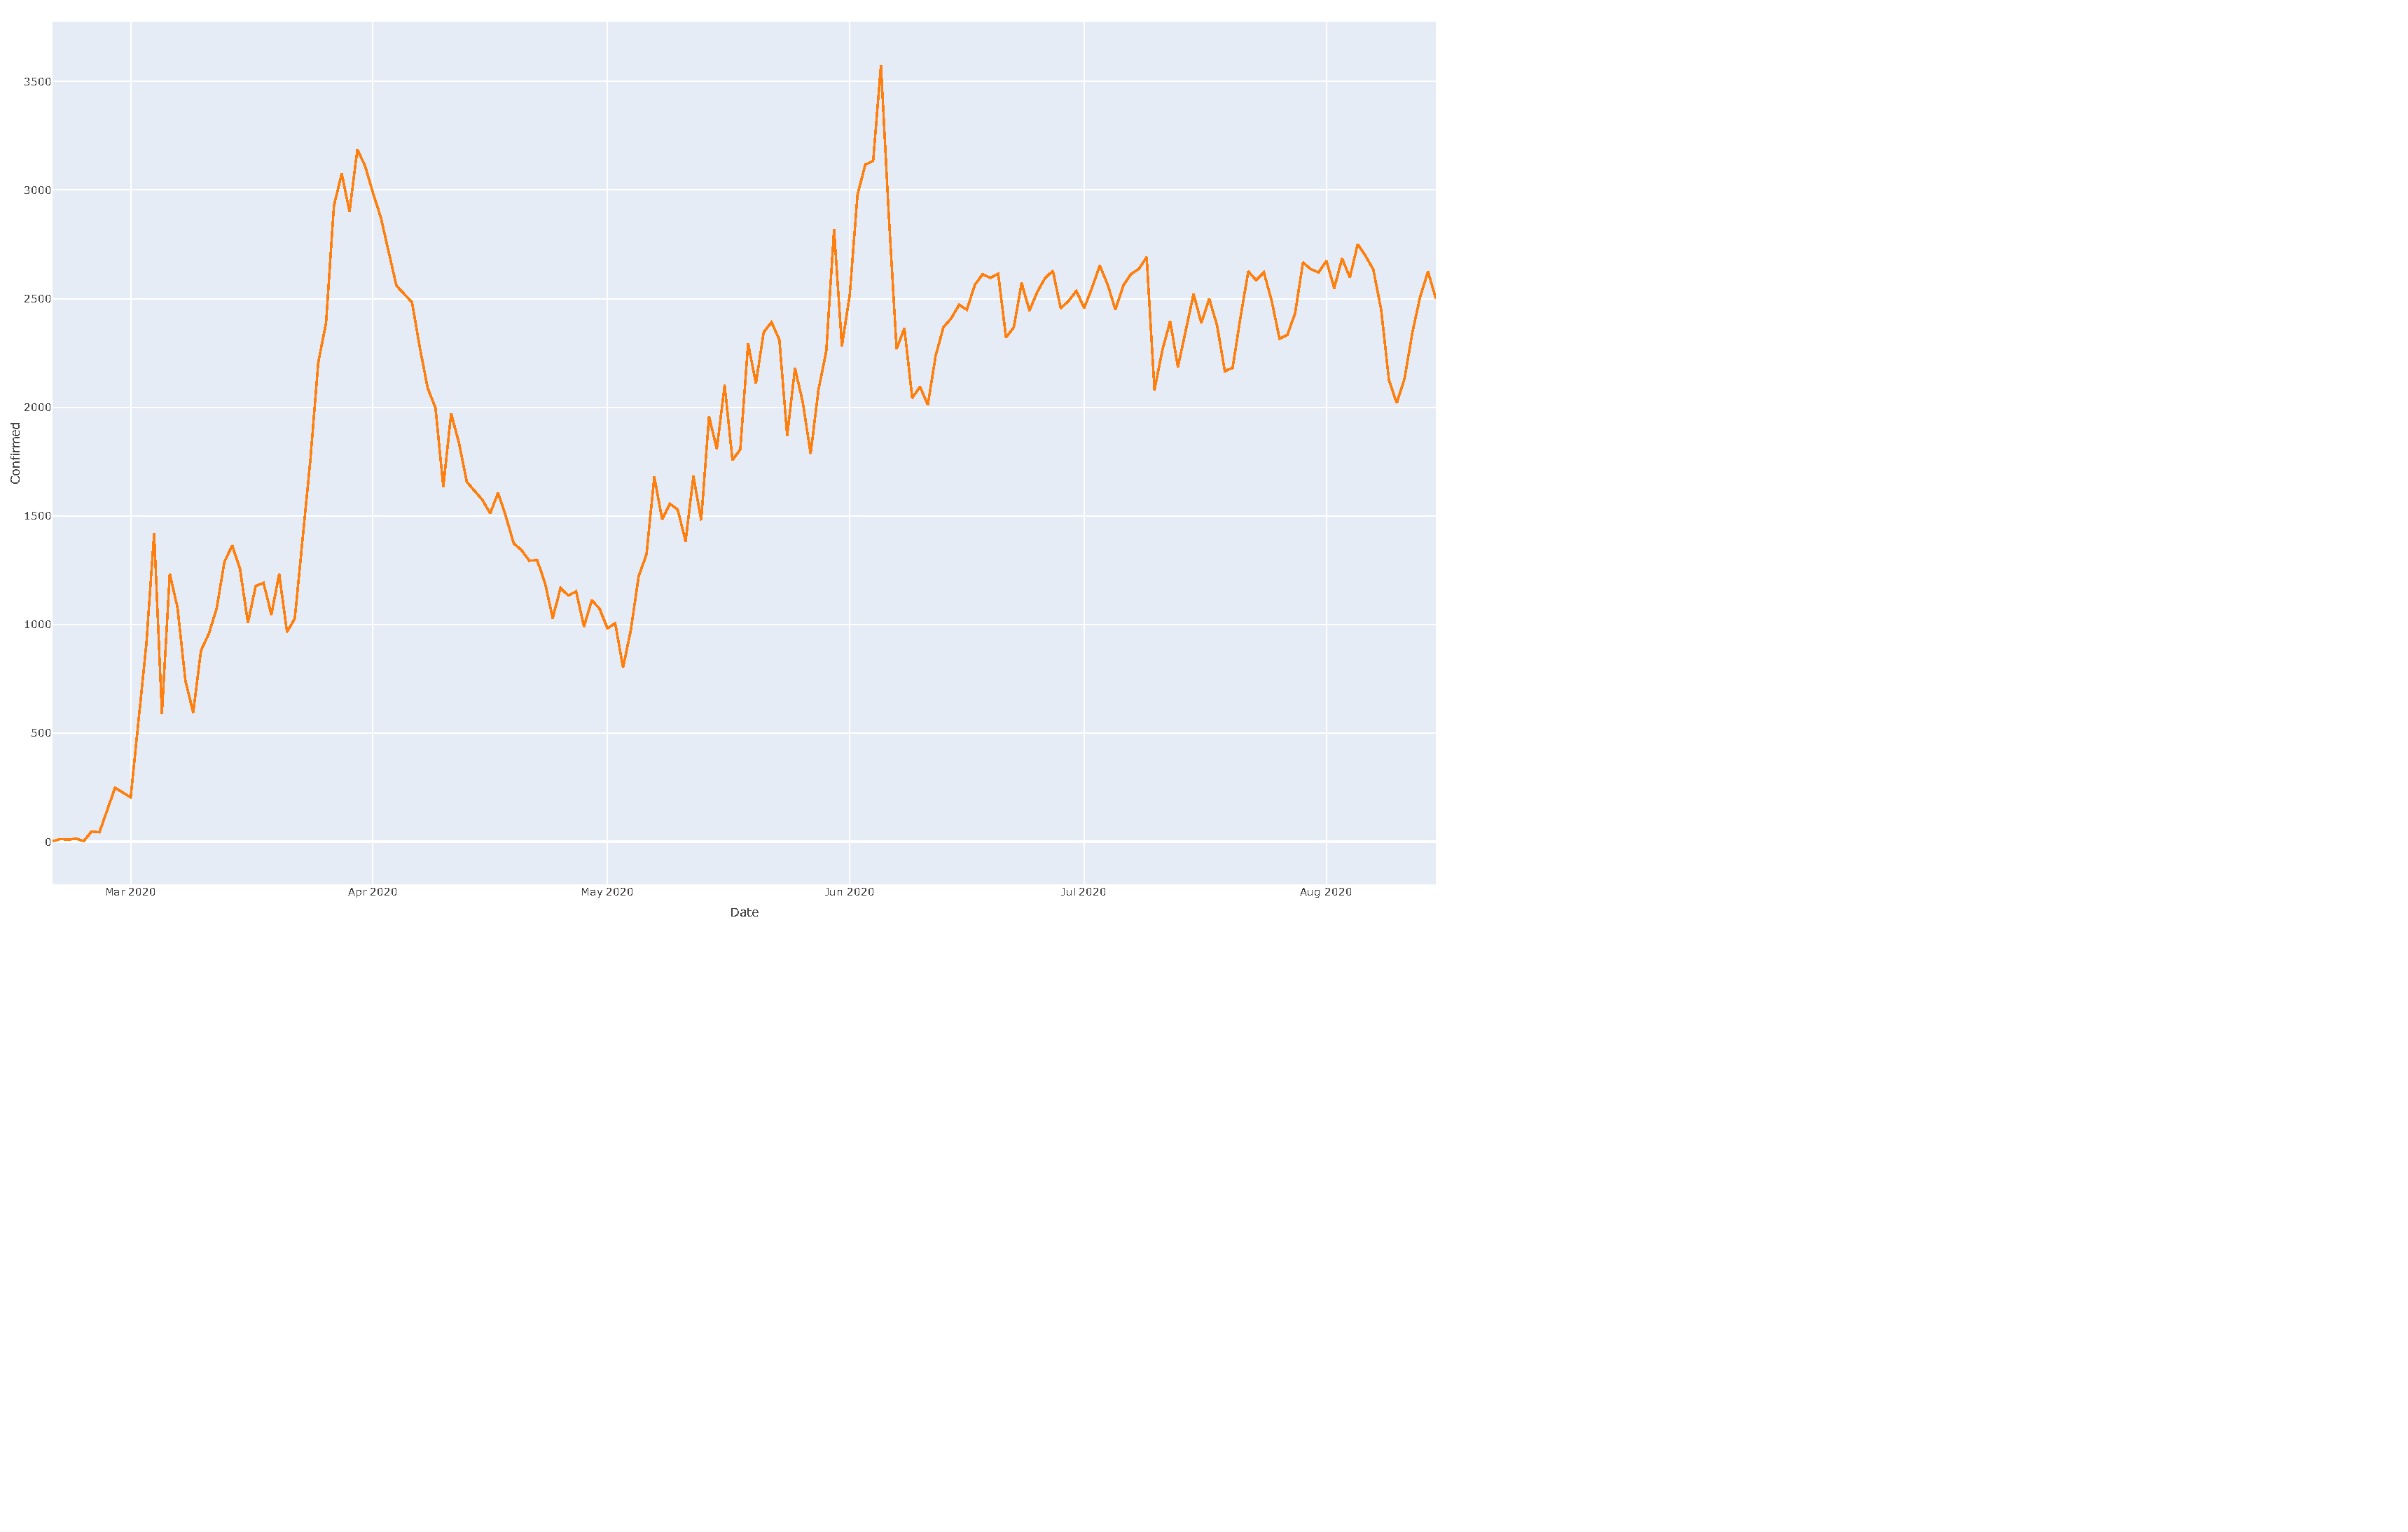
\includegraphics{confirmados_files/figure-pdf/unnamed-chunk-9-1.pdf}

}

\caption{\label{fig-box}Boxplot de casos confirmados de COVID-19 en Irán
del 20-02-2020 al 15-08-2020}

\end{figure}%

\subsection{Componentes de la serie de
tiempo}\label{componentes-de-la-serie-de-tiempo}

Los componentes identificados en la serie de tiempo de casos confirmados
de COVID-19 en Irán, revelan distintos patrones y características.

En primer lugar, se observa una \textbf{tendencia} discernible en el
gráfico de la serie temporal (Figura~\ref{fig-ts}). Por ejemplo, entre
el 30 de marzo y el 03 de mayo de 2020, se evidencia una tendencia
negativa o decreciente, seguida por una tendencia creciente a partir del
03 de mayo en adelante. Estos cambios en la tendencia podrían indicar
fluctuaciones significativas en la evolución de los casos confirmados
durante esos periodos específicos.

En cuanto a la \textbf{estacionalidad}, aunque no se identifica
claramente a simple vista en el periodo observado, la extensión del
análisis a un periodo más amplio podría revelar patrones recurrentes o
ciclos temporales característicos. Es posible que ciertos patrones
estacionales se manifiesten en intervalos más extensos de la serie
temporal, lo que implicaría variaciones sistemáticas y repetitivas en
los datos en períodos específicos.

Por último, se destacan pequeñas subidas y bajadas en el gráfico que
sugieren la presencia de \textbf{ruido} en la serie temporal. Estas
fluctuaciones irregulares podrían atribuirse a diversas causas, como
posibles errores en la recolección de datos o fluctuaciones aleatorias
inherentes al comportamiento de la enfermedad. Es importante considerar
estas variaciones no sistemáticas al analizar la serie temporal, ya que
podrían influir en la interpretación de los patrones y tendencias
observadas.

\subsection{Estacionariedad}\label{estacionariedad}

A continuación, se emplea el test de \textbf{Dickey-Fuller} para
examinar la presencia de estacionariedad en la serie temporal. Este test
fue utilizado con la finalidad de identificar la existencia de raíces
unitarias en la serie, lo cual permite inferir la presencia o ausencia
de estacionariedad en los datos analizados.

\begin{Shaded}
\begin{Highlighting}[]
\FunctionTok{adf.test}\NormalTok{(Confirmed\_ts, }\AttributeTok{alternative =} \StringTok{"stationary"}\NormalTok{)}
\end{Highlighting}
\end{Shaded}

\begin{verbatim}

    Augmented Dickey-Fuller Test

data:  Confirmed_ts
Dickey-Fuller = -2.9529, Lag order = 5, p-value = 0.1781
alternative hypothesis: stationary
\end{verbatim}

La hipótesis nula \((H_0)\) asume la presencia de raíces unitarias, lo
que indica no estacionariedad en la serie. Al obtener un \(p-\)valor
superior al nivel de significancia establecido el cuál es del \(95\%\),
no se rechaza la hipótesis nula, sugiriendo la ausencia de
estacionariedad en la serie de tiempo de casos confirmados.

Además, se complementa la evaluación de la estacionalidad mediante la
inspección de los gráficos de la función de autocorrelación (ACF) y la
función de autocorrelación parcial (PACF). Estos gráficos se utilizan
para identificar patrones de autocorrelación en la serie temporal, lo
que permite visualizar la presencia de estacionalidad, tendencias o
ciclos.

La serie de tiempo representada en la Figura~\ref{fig-ts} exhibe un
comportamiento característico de deambulación aleatoria. Dado que el
valor de la variable \(X_{t+1}\) generalmente se encuentra en proximidad
al valor \(X_t\), se evidencia una autocorrelación positiva notablemente
marcada entre las variables \(X_t\) y \(X_{t+1}\).

\begin{Shaded}
\begin{Highlighting}[]
\FunctionTok{autoplot}\NormalTok{(}\FunctionTok{acf}\NormalTok{(Confirmed\_ts, }\AttributeTok{plot =} \ConstantTok{FALSE}\NormalTok{), }
         \AttributeTok{main=}\StringTok{"Autocorrelograma de casos confirmados"}\NormalTok{)}
\end{Highlighting}
\end{Shaded}

\begin{figure}

\centering{

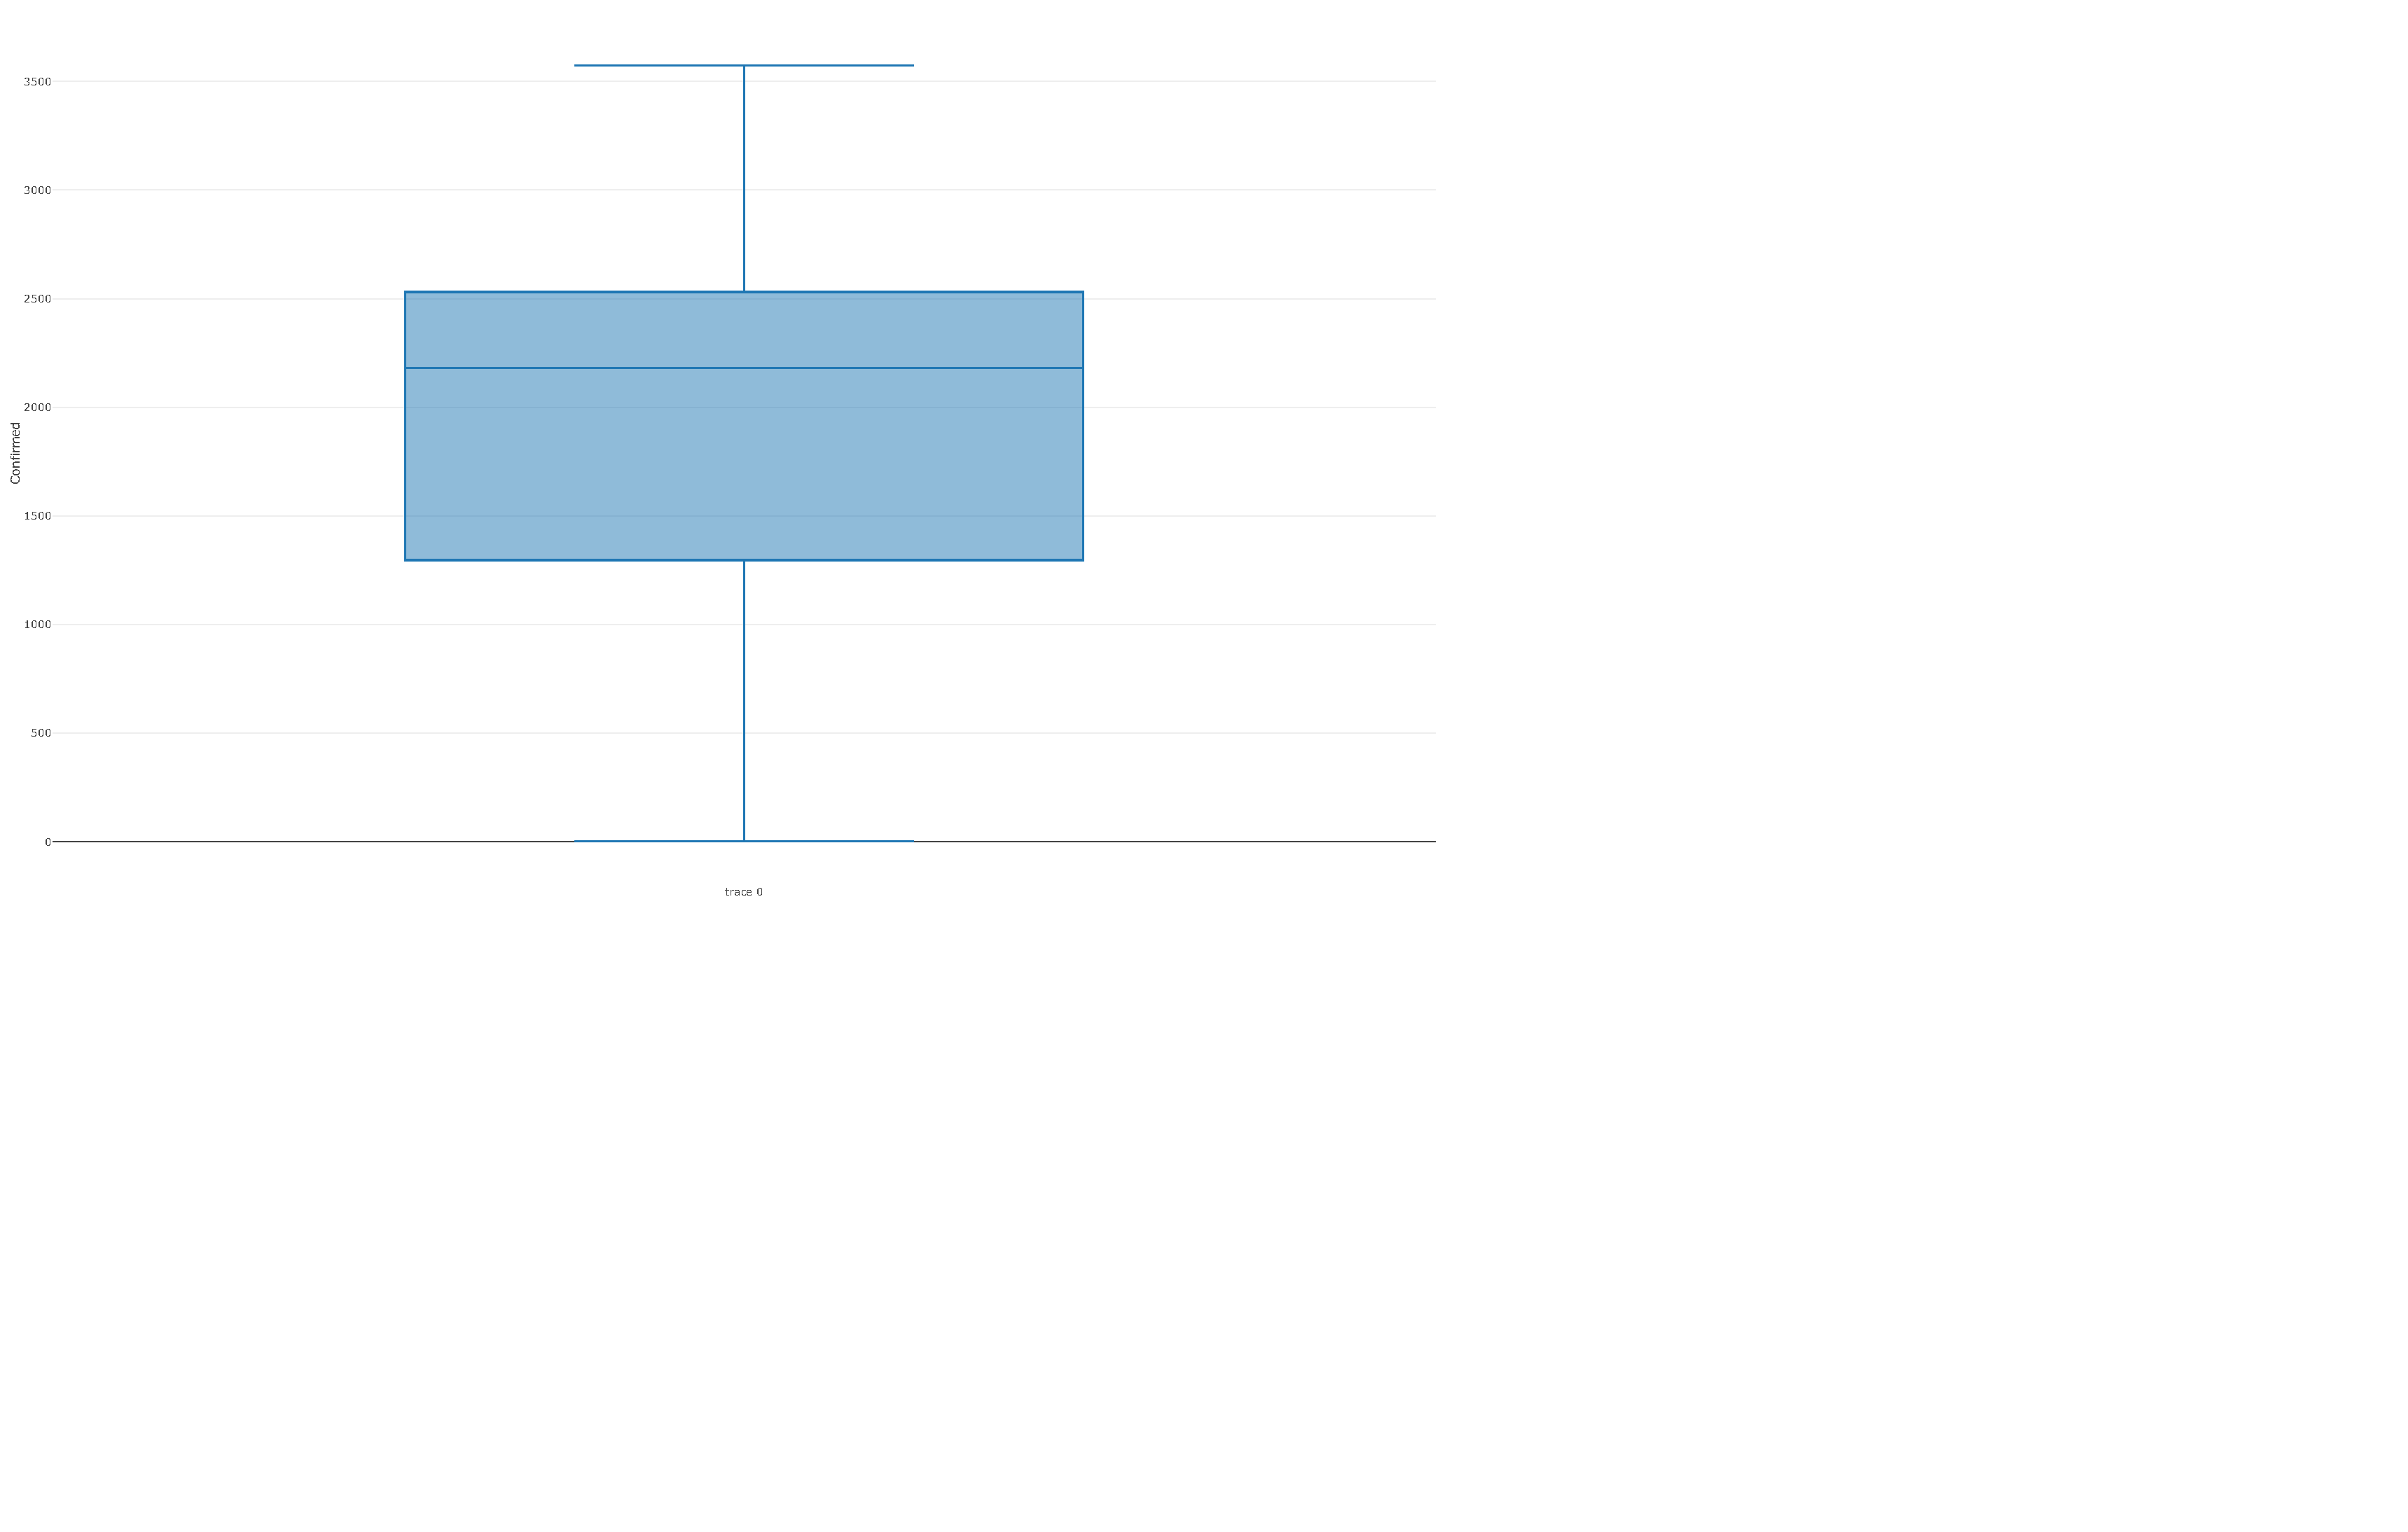
\includegraphics{confirmados_files/figure-pdf/unnamed-chunk-11-1.pdf}

}

\caption{\label{fig-acf}Autocorrelograma de los casos confirmados de
COVID-19 en Irán}

\end{figure}%

En la Figura~\ref{fig-acf} se observa que la \textbf{autocorrelación}
entre \(X_t\) y \(X_{t+k}\) decrece con el incremento del retraso \(k\).
Este declive conduce a la constatación de que, a un desfase de \(20\),
existe una correlación bastante débil entre \(X_t\) y \(X_{t+20}\). Al
analizar el gráfico de la función de autocorrelación (ACF), se aprecia
que \(\rho_{20}\approx 0.19\).

La gráfica de la \textbf{Función de Autocorrelación Parcial} (PACF)
proporciona información valiosa sobre la estructura de autocorrelación
de una serie temporal una vez han sido eliminadas las correlaciones
debidas a los intervalos de tiempo intermedios.

\begin{Shaded}
\begin{Highlighting}[]
\FunctionTok{ggPacf}\NormalTok{((Confirmed\_ts), }\AttributeTok{main =} \StringTok{\textquotesingle{}Autocorrelograma parcial de casos confirmados\textquotesingle{}}\NormalTok{)}
\end{Highlighting}
\end{Shaded}

\begin{figure}

\centering{

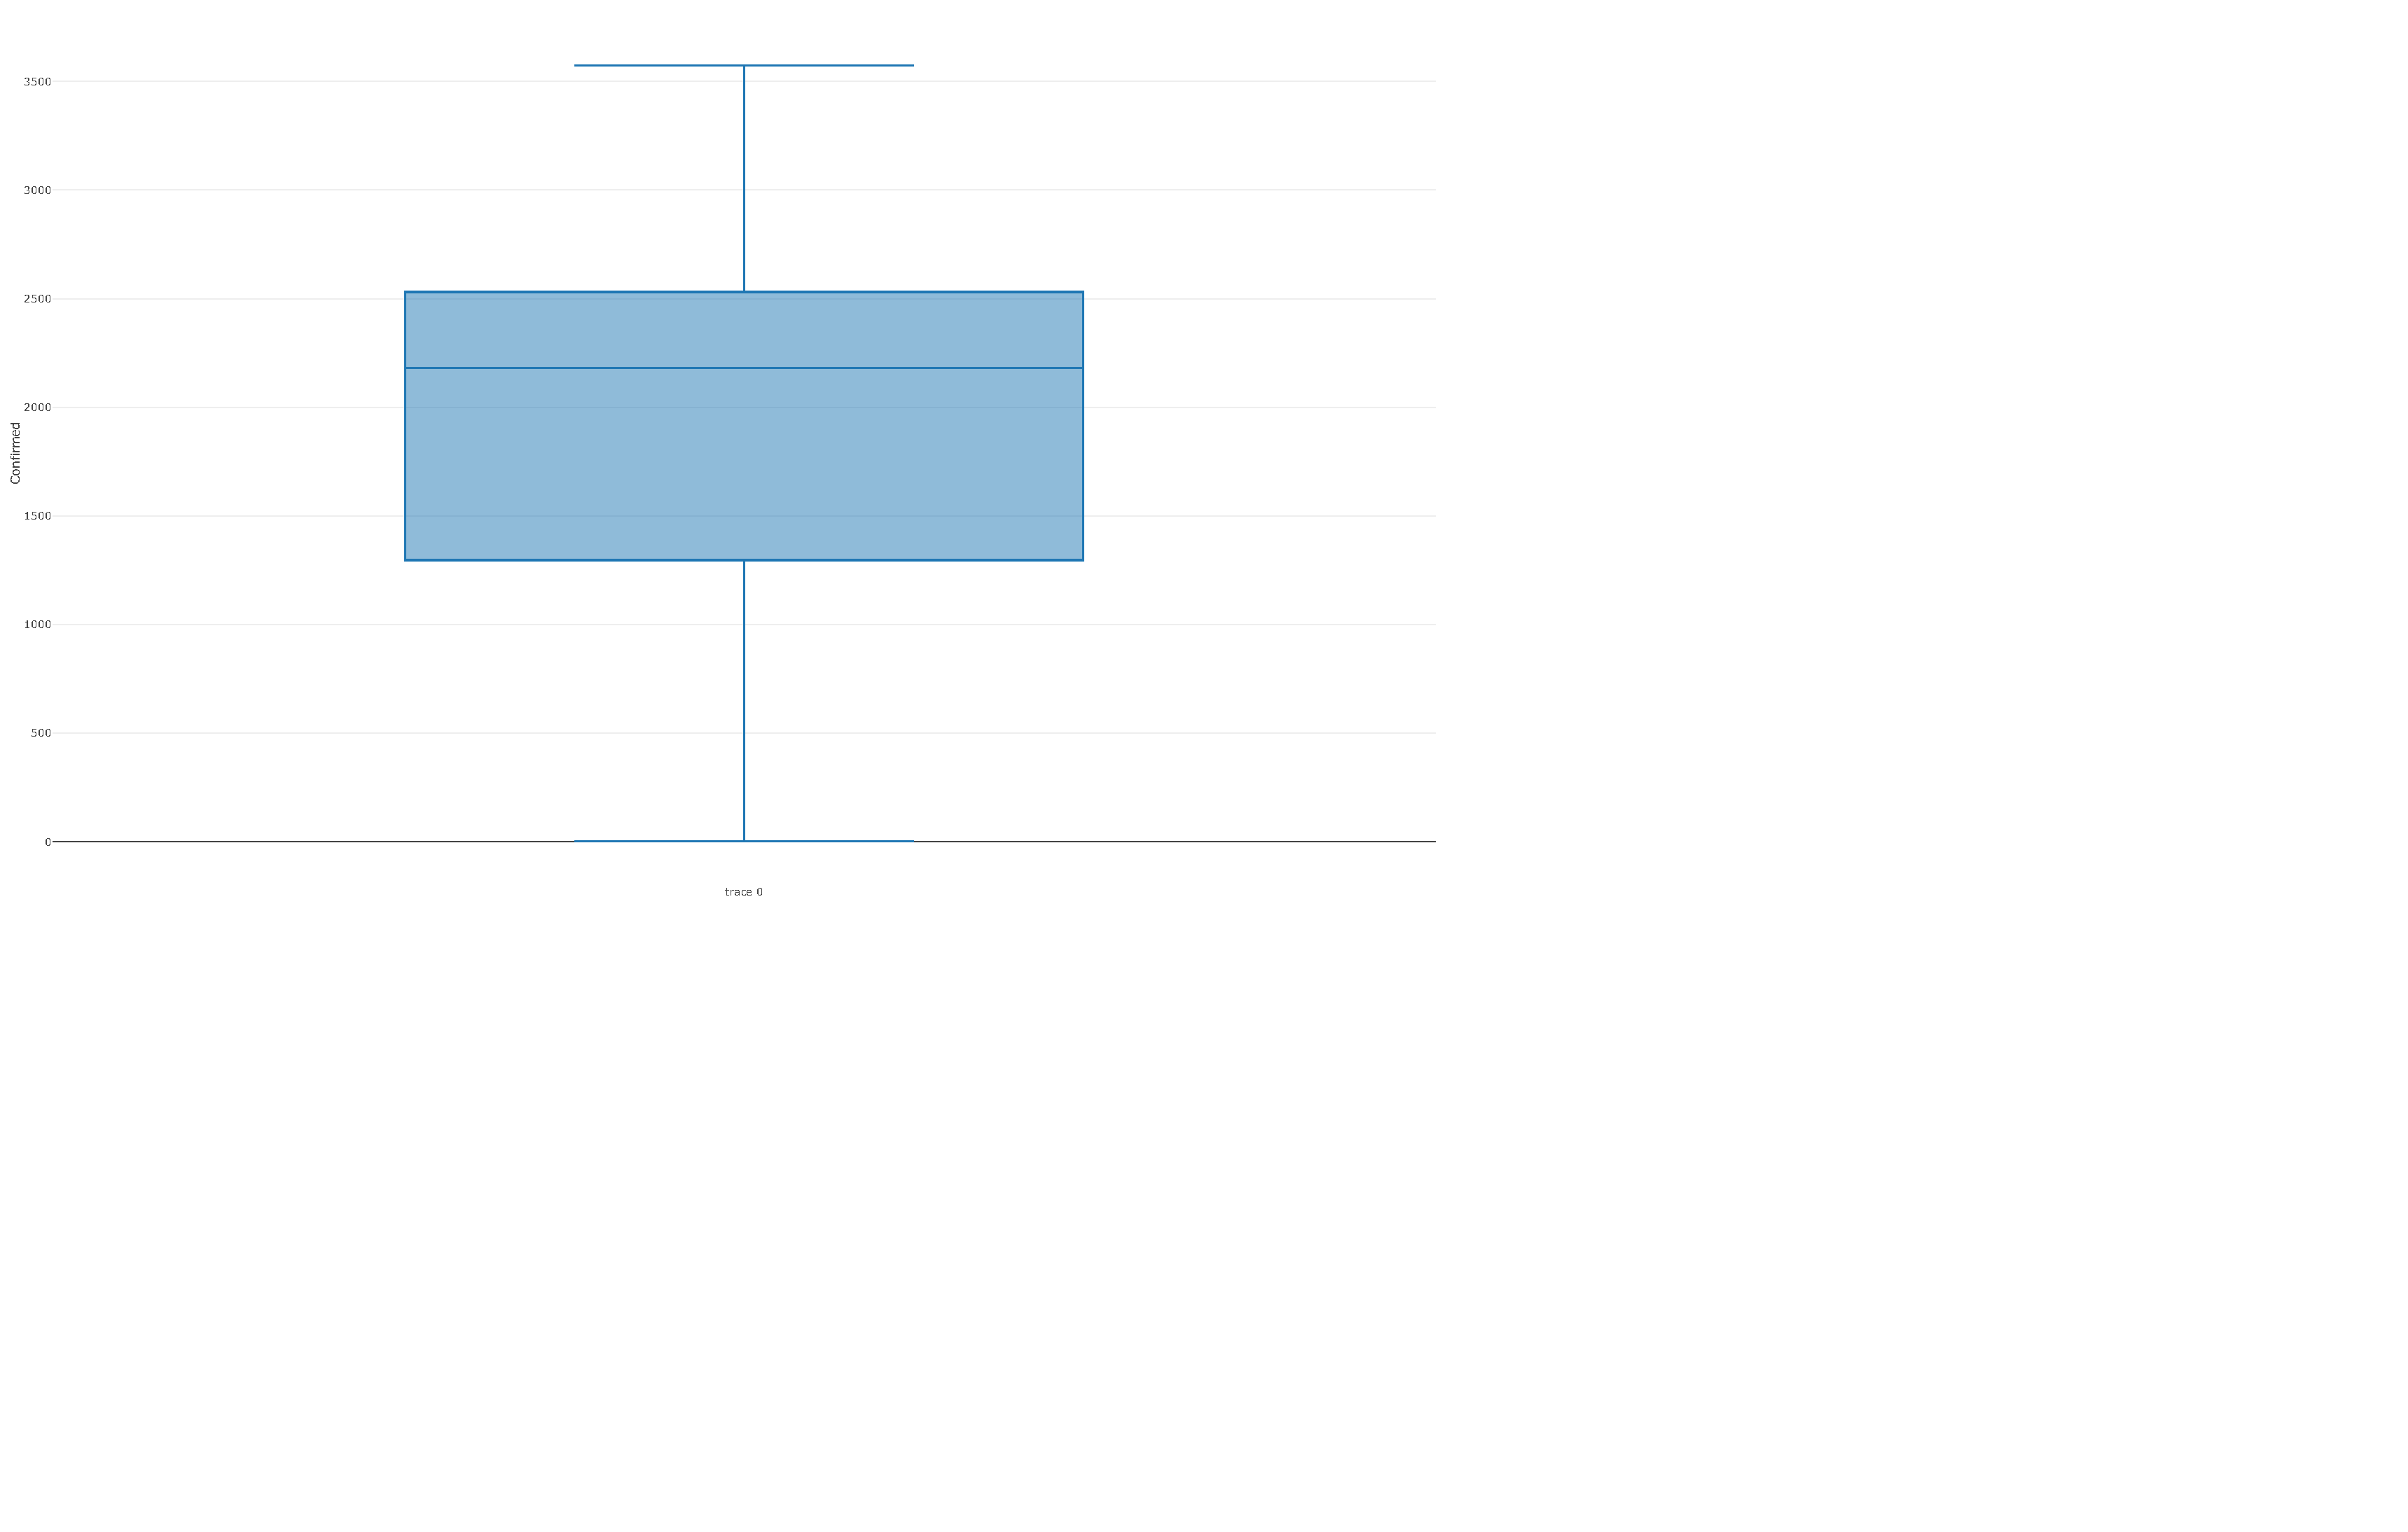
\includegraphics{confirmados_files/figure-pdf/unnamed-chunk-12-1.pdf}

}

\caption{\label{fig-pacf}Autocorrelograma Parcial de los casos
confirmados de COVID-19 en Irán}

\end{figure}%

La Figura~\ref{fig-pacf} indica que el valor de \(\phi_{15}\) es
ligeramente superior a \(0.25\), aproximadamente
\(\phi_{52}\approx 0.16\), y \(\phi_{76}\approx 0.15\), mientras que
para los restantes valores, la correlación parcial no es nula.

\begin{remark}
De acuerdo con la gráfica de la Función de Autocorrelación Parcial
Figura~\ref{fig-pacf}, se observa un corte abrupto después del rezago 4,
lo cual sugiere que las autocorrelaciones parciales más allá de ese
punto no poseen significancia estadística. Por consiguiente, se infiere
la posibilidad de ajustar un modelo autoregresivo AR(4) a la base de
datos.

\begin{Shaded}
\begin{Highlighting}[]
\FunctionTok{library}\NormalTok{(tswge)}
\NormalTok{coeff }\OtherTok{\textless{}{-}} \FunctionTok{est.ar.wge}\NormalTok{(Confirmed\_ts, }\AttributeTok{p=}\DecValTok{4}\NormalTok{)}
\end{Highlighting}
\end{Shaded}

\begin{verbatim}
  
  
Coefficients of AR polynomial:  
0.8656 0.1724 0.0592 -0.1318 

                           AR Factor Table 
Factor                 Roots                Abs Recip    System Freq 
1-0.9605B              1.0411               0.9605       0.0000
1-0.5355B              1.8675               0.5355       0.0000
1+0.6303B+0.2563B^2   -1.2298+-1.5459i      0.5062       0.3570
  
  
\end{verbatim}

\begin{Shaded}
\begin{Highlighting}[]
\NormalTok{coeff}\SpecialCharTok{$}\NormalTok{phi }\CommentTok{\#coeficientes}
\end{Highlighting}
\end{Shaded}

\begin{verbatim}
[1]  0.86563811  0.17237111  0.05917558 -0.13180534
\end{verbatim}

\begin{Shaded}
\begin{Highlighting}[]
\NormalTok{coeff}\SpecialCharTok{$}\NormalTok{xbar }\CommentTok{\#media}
\end{Highlighting}
\end{Shaded}

\begin{verbatim}
[1] 1922.868
\end{verbatim}

\begin{Shaded}
\begin{Highlighting}[]
\NormalTok{coeff}\SpecialCharTok{$}\NormalTok{avar }\CommentTok{\#varianza finita}
\end{Highlighting}
\end{Shaded}

\begin{verbatim}
[1] 47818.04
\end{verbatim}

El modelo autoregresivo AR(4) se expresa mediante la siguiente ecuación:

\begin{equation}\phantomsection\label{eq-AR4}{
(1-0.865B-0.172B^2-0.059B^3+0.131B^4)(X_t-1922.868)+a_t
}\end{equation}

donde \(\hat{\sigma}_a^2 = 47818.04\).
\end{remark}

El análisis del ACF y PACF proporcionó información sobre la relación de
los puntos de datos con sus rezagos, permitiendo observar posibles
patrones estacionales. La presencia de picos significativos en estos
gráficos podría indicar la existencia de estacionalidad en la serie de
tiempo.

\section{Entrenamiento, modelado, pronóstico y métricas de
rendimiento}\label{entrenamiento-modelado-pronuxf3stico-y-muxe9tricas-de-rendimiento}

Se procede a la evaluación del desempeño de los métodos a través de la
separación del conjunto de datos en entrenamiento y prueba. El set
inicial, compuesto por el \(70\%\) de los datos, se emplea para el
entrenamiento de los modelos, mientras que el \(30\%\) restante se
reservará para llevar a cabo las pruebas pertinentes.

\begin{Shaded}
\begin{Highlighting}[]
\NormalTok{Confirmed\_ts }\OtherTok{\textless{}{-}} \FunctionTok{ts}\NormalTok{(Confirmed\_ts,}\AttributeTok{frequency=}\DecValTok{1}\NormalTok{)}
\NormalTok{tsize }\OtherTok{\textless{}{-}} \FunctionTok{round}\NormalTok{(}\FloatTok{0.7} \SpecialCharTok{*} \FunctionTok{nrow}\NormalTok{(Confirmed\_df))}
\NormalTok{train\_confirmed }\OtherTok{\textless{}{-}} \FunctionTok{window}\NormalTok{(Confirmed\_ts,}\AttributeTok{end=}\NormalTok{tsize)}
\NormalTok{test\_confirmed }\OtherTok{\textless{}{-}} \FunctionTok{window}\NormalTok{(Confirmed\_ts,}\AttributeTok{start=}\NormalTok{tsize}\SpecialCharTok{+}\DecValTok{1}\NormalTok{)}
\end{Highlighting}
\end{Shaded}

\subsection{Holt-Winters}\label{sec-holt-winters}

Con el fin de determinar la descomposición más adecuada para los datos
en cuestión, se empleó un criterio elaborado basado en el coeficiente de
variación, el cual proporciona una recomendación entre las dos versiones
disponibles.

\begin{Shaded}
\begin{Highlighting}[]
\NormalTok{DescRec }\OtherTok{\textless{}{-}} \ControlFlowTok{function}\NormalTok{(x)\{}
\NormalTok{  n }\OtherTok{=} \FunctionTok{length}\NormalTok{(x)}
\NormalTok{  di }\OtherTok{=} \FunctionTok{rep}\NormalTok{(}\DecValTok{0}\NormalTok{, n}\DecValTok{{-}1}\NormalTok{)}
\NormalTok{  ci }\OtherTok{=} \FunctionTok{rep}\NormalTok{(}\DecValTok{0}\NormalTok{, n}\DecValTok{{-}1}\NormalTok{)}
  \ControlFlowTok{for}\NormalTok{ (i }\ControlFlowTok{in} \DecValTok{1}\SpecialCharTok{:}\NormalTok{n}\DecValTok{{-}1}\NormalTok{) \{}
\NormalTok{    di[i] }\OtherTok{=}\NormalTok{ x[i}\SpecialCharTok{+}\DecValTok{1}\NormalTok{] }\SpecialCharTok{{-}}\NormalTok{ x[i]}
\NormalTok{    ci[i] }\OtherTok{=}\NormalTok{ x[i}\SpecialCharTok{+}\DecValTok{1}\NormalTok{] }\SpecialCharTok{/}\NormalTok{ x[i]}
\NormalTok{  \}}
\NormalTok{  d }\OtherTok{\textless{}{-}} \FunctionTok{cv}\NormalTok{(di) }
\NormalTok{  c }\OtherTok{\textless{}{-}} \FunctionTok{cv}\NormalTok{(ci) }\SpecialCharTok{/} \FunctionTok{mean}\NormalTok{(di)}
  \ControlFlowTok{if}\NormalTok{(d }\SpecialCharTok{\textless{}}\NormalTok{ c)}
    \FunctionTok{print}\NormalTok{(}\StringTok{"Se recomienda la descomposición aditiva"}\NormalTok{)}
  \ControlFlowTok{else}
    \FunctionTok{print}\NormalTok{(}\StringTok{"Se recomienda la descomposición multiplicativa"}\NormalTok{)}
\NormalTok{\}}
\FunctionTok{DescRec}\NormalTok{(train\_confirmed)}
\end{Highlighting}
\end{Shaded}

\begin{verbatim}
[1] "Se recomienda la descomposición multiplicativa"
\end{verbatim}

De acuerdo con la recomendación observada, se sugiere la utilización de
la versión \textbf{multiplicativa}. En consecuencia, se procede a
mostrar la representación gráfica de la descomposición multiplicativa de
la serie temporal.

\begin{Shaded}
\begin{Highlighting}[]
\NormalTok{ts\_train }\OtherTok{\textless{}{-}} \FunctionTok{ts}\NormalTok{(train\_confirmed, }\AttributeTok{frequency =} \DecValTok{2}\NormalTok{)}
\NormalTok{components\_ts }\OtherTok{\textless{}{-}} \FunctionTok{decompose}\NormalTok{(ts\_train, }\AttributeTok{type =} \StringTok{\textquotesingle{}mult\textquotesingle{}}\NormalTok{)}
\FunctionTok{plot}\NormalTok{(components\_ts)}
\end{Highlighting}
\end{Shaded}

\begin{figure}

\centering{

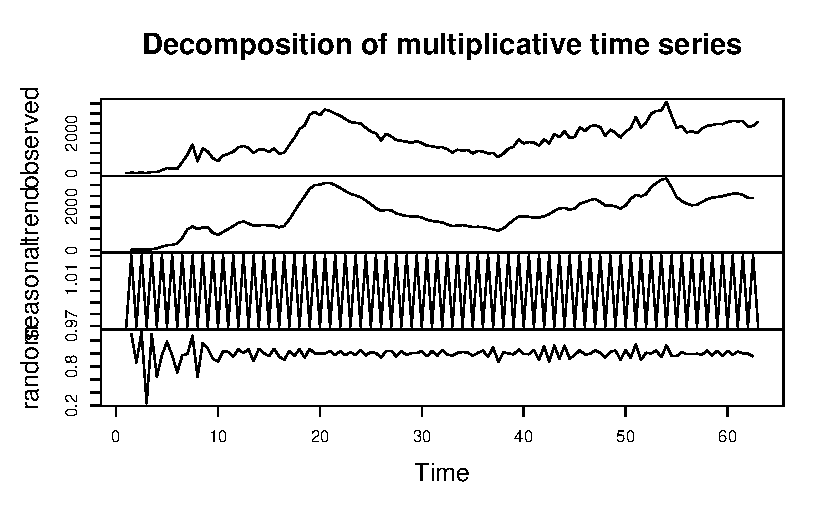
\includegraphics{confirmados_files/figure-pdf/unnamed-chunk-16-1.pdf}

}

\caption{\label{fig-descomp}Descomposición multiplicativa de la serie de
tiempo}

\end{figure}%

Se procede ahora a la aplicación del modelo multiplicativo de
Holt-Winters a la serie temporal de los datos de entrenamiento
utilizando una frecuencia de dos, con el fin de permitir la
aplicabilidad del modelo.

\begin{Shaded}
\begin{Highlighting}[]
\NormalTok{HWc }\OtherTok{\textless{}{-}} \FunctionTok{HoltWinters}\NormalTok{(ts\_train, }\AttributeTok{seasonal =} \StringTok{\textquotesingle{}mult\textquotesingle{}}\NormalTok{)}
\NormalTok{HWc}
\end{Highlighting}
\end{Shaded}

\begin{verbatim}
Holt-Winters exponential smoothing with trend and multiplicative seasonal component.

Call:
HoltWinters(x = ts_train, seasonal = "mult")

Smoothing parameters:
 alpha: 0.729859
 beta : 0
 gamma: 0.6494094

Coefficients:
          [,1]
a  2289.283568
b     2.250000
s1    1.119185
s2    1.113547
\end{verbatim}

Finalmente, utilizando el modelo de entrenamiento desarrollado en la
fase previa, se lleva a cabo la proyección con un horizonte de
predicción igual en extensión a los datos de prueba, acompañado de un
intervalo de confianza que oscila entre el \(80\%\) y el \(95\%\).

\begin{Shaded}
\begin{Highlighting}[]
\NormalTok{HWc\_for }\OtherTok{\textless{}{-}} \FunctionTok{forecast}\NormalTok{(HWc, }\AttributeTok{h=}\FunctionTok{length}\NormalTok{(test\_confirmed))}
\end{Highlighting}
\end{Shaded}

\begin{tcolorbox}[enhanced jigsaw, titlerule=0mm, left=2mm, opacityback=0, toprule=.15mm, colframe=quarto-callout-note-color-frame, bottomrule=.15mm, breakable, coltitle=black, opacitybacktitle=0.6, bottomtitle=1mm, colback=white, arc=.35mm, leftrule=.75mm, toptitle=1mm, colbacktitle=quarto-callout-note-color!10!white, title=\textcolor{quarto-callout-note-color}{\faInfo}\hspace{0.5em}{Nota}, rightrule=.15mm]

Las funciones aplicadas en esta sección son parte de la librería
\textbf{\emph{stats}} (2023) de R.

\end{tcolorbox}

\subsection{MLP}\label{mlp-1}

Posteriormente, se procede al entrenamiento del modelo MLP (Perceptrón
Multicapa). La cantidad de capas ocultas y la configuración de nodos en
cada capa se determinaron de manera automatizada mediante el método de
validación cruzada de 5 pliegues. Asimismo, se eligió la función de
activación como sigmoide, y el proceso de entrenamiento del modelo se
ejecutó a lo largo de 20 iteraciones.2

\begin{Shaded}
\begin{Highlighting}[]
\NormalTok{fitc }\OtherTok{\textless{}{-}} \FunctionTok{mlp}\NormalTok{(train\_confirmed, }\AttributeTok{hd.auto.type=}\StringTok{"cv"}\NormalTok{, }\AttributeTok{reps =} \DecValTok{20}\NormalTok{, }\AttributeTok{comb =} \StringTok{\textquotesingle{}median\textquotesingle{}}\NormalTok{)}
\NormalTok{fitc}
\end{Highlighting}
\end{Shaded}

\begin{verbatim}
MLP fit with 1 hidden node and 20 repetitions.
Univariate lags: (1,2,4)
Forecast combined using the median operator.
MSE: 57284.6891.
\end{verbatim}

\begin{Shaded}
\begin{Highlighting}[]
\FunctionTok{plot}\NormalTok{(fitc)}
\end{Highlighting}
\end{Shaded}

\begin{figure}

\centering{

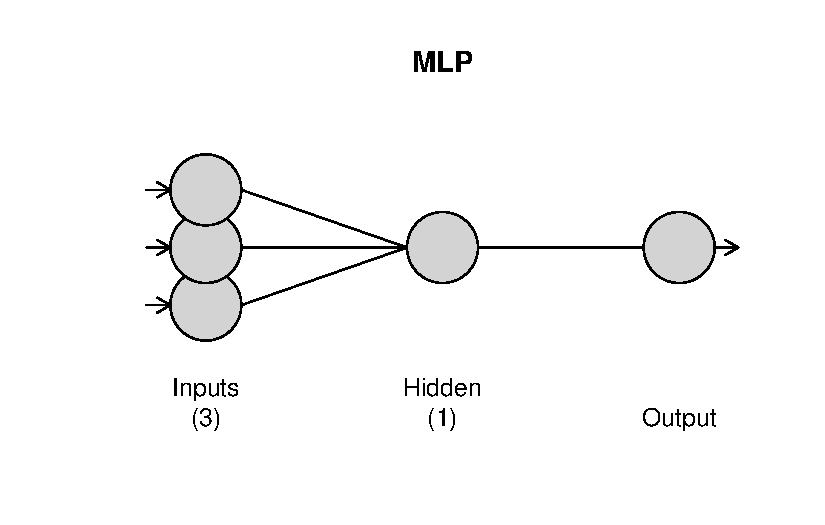
\includegraphics{confirmados_files/figure-pdf/unnamed-chunk-20-1.pdf}

}

\caption{\label{fig-red}Estructura de la red neuronal resultante}

\end{figure}%

Para llevar a cabo el pronóstico, se emplea el modelo de entrenamiento
creado en la etapa anterior, manteniendo un horizonte de predicción que
coincide en duración con los datos de prueba, tal como se hizo con la
técnica anterior.

\begin{Shaded}
\begin{Highlighting}[]
\NormalTok{frcc }\OtherTok{\textless{}{-}} \FunctionTok{forecast}\NormalTok{(fitc,}\AttributeTok{h=}\FunctionTok{length}\NormalTok{(test\_confirmed))}
\end{Highlighting}
\end{Shaded}

\begin{tcolorbox}[enhanced jigsaw, titlerule=0mm, left=2mm, opacityback=0, toprule=.15mm, colframe=quarto-callout-note-color-frame, bottomrule=.15mm, breakable, coltitle=black, opacitybacktitle=0.6, bottomtitle=1mm, colback=white, arc=.35mm, leftrule=.75mm, toptitle=1mm, colbacktitle=quarto-callout-note-color!10!white, title=\textcolor{quarto-callout-note-color}{\faInfo}\hspace{0.5em}{Nota}, rightrule=.15mm]

Las funciones aplicadas en esta sección son parte de la librería
\textbf{\emph{nnfor}} (Kourentzes 2022) de R.

\end{tcolorbox}

\subsection{Comparación de pronósticos con el conjunto de datos de
prueba}\label{comparaciuxf3n-de-pronuxf3sticos-con-el-conjunto-de-datos-de-prueba}

Con el propósito de llevar a cabo un análisis cuantitativo exhaustivo,
se presenta a continuación una tabla comparativa de los resultados
derivados de las dos técnicas implementadas y la base de datos de
prueba. Posteriormente, se exhiben gráficas representativas de estos
resultados. En la Figura~\ref{fig-phw} se muestra el pronóstico mediante
Holt-Winters acompañado de su respectivo intervalo de confianza. En
contraste, en la Figura~\ref{fig-pmlp}, la gráfica punteada en color
rojo representa el comportamiento real de los datos, mientras que en
azul se representa el pronóstico obtenido a través de la red MLP.

\begin{table}

\caption{\label{tbl-forecast}Comparación de Resultados entre las
técnicas y los datos reales para evaluar precisión}

\centering{


\includegraphics{confirmados_files/figure-pdf/tbl-forecast-1.pdf}

}

\end{table}%

\begin{figure}

\centering{

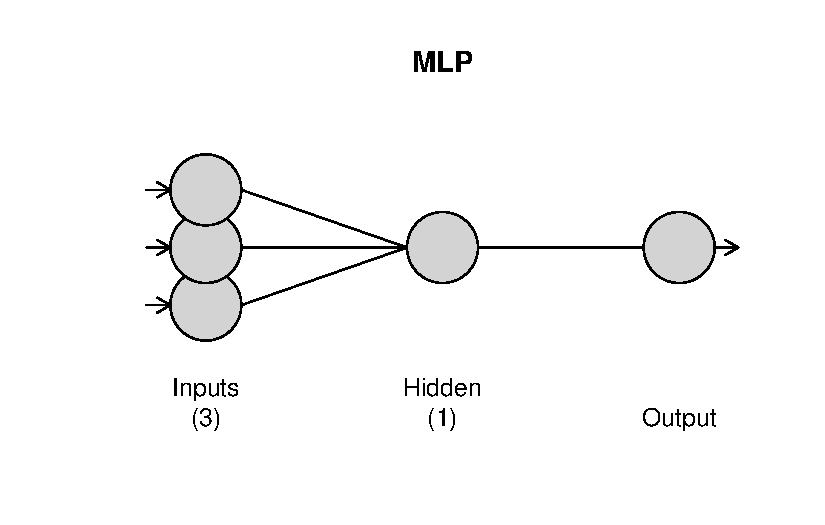
\includegraphics{confirmados_files/figure-pdf/unnamed-chunk-23-1.pdf}

}

\caption{\label{fig-phw}Pronóstico obtenido mediante la técnica de
Holt-Winters.}

\end{figure}%

\begin{figure}

\centering{

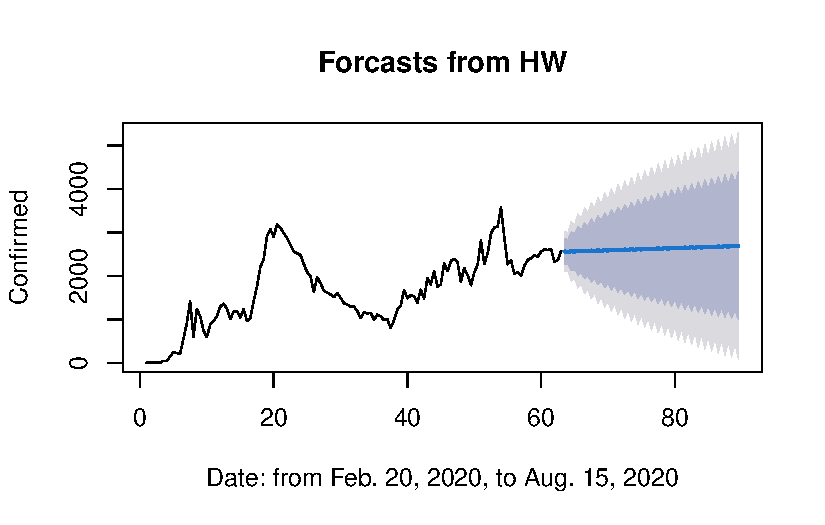
\includegraphics{confirmados_files/figure-pdf/unnamed-chunk-24-1.pdf}

}

\caption{\label{fig-pmlp}Pronóstico obtenido mediante la red neuronal
MLP.}

\end{figure}%

\subsubsection{Métricas de
rendimiento}\label{muxe9tricas-de-rendimiento}

Para evaluar la calidad o bondad de ajuste de los métodos utilizados en
este estudio y seleccionar el modelo más apropiado, se aplican tres
métricas de rendimiento, Error Cuadrático Medio (RMSE), Error Absoluto
Medio (MAE) y Error Porcentual Absoluto Medio (MAPE) tanto en las fases
de entrenamiento como en las de prueba. Los resultados correspondientes
a éstas métricas se presentan en la Tabla~\ref{tbl-err} . Estas medidas
se definen de la siguiente manera:

\begin{equation}\phantomsection\label{eq-metricas}{
\begin{split}\text{RMSE}&=\sqrt{\frac{1}{N}\sum_{i=1}^N (y_i-\hat{y_i})^2}\\ \text{MAE}&=\frac{1}{N}\sum_{i=1}^N |y_i-\hat{y_i}|\\ 
\text{MAPE}&=\frac{1}{N}\sum_{i=1}^N\frac{|y_i-\hat{y_i}|}{y_i}*100\end{split}
}\end{equation}

donde \(y_i\) representa el valor real de la serie temporal en el
instante \(i\), y \(\hat{y_i}\) denota el valor predicho de la serie de
tiempo en el instante \(i\).

\begin{longtable}[]{@{}
  >{\raggedright\arraybackslash}p{(\columnwidth - 12\tabcolsep) * \real{0.1624}}
  >{\centering\arraybackslash}p{(\columnwidth - 12\tabcolsep) * \real{0.1282}}
  >{\centering\arraybackslash}p{(\columnwidth - 12\tabcolsep) * \real{0.1453}}
  >{\centering\arraybackslash}p{(\columnwidth - 12\tabcolsep) * \real{0.1282}}
  >{\centering\arraybackslash}p{(\columnwidth - 12\tabcolsep) * \real{0.1282}}
  >{\centering\arraybackslash}p{(\columnwidth - 12\tabcolsep) * \real{0.1368}}
  >{\centering\arraybackslash}p{(\columnwidth - 12\tabcolsep) * \real{0.1282}}@{}}
\caption{Errores de los modelos para casos
confirmados.}\label{tbl-err}\tabularnewline
\toprule\noalign{}
\endfirsthead
\endhead
\bottomrule\noalign{}
\endlastfoot
& & \textbf{\emph{Training}} & & & \textbf{\emph{Testing}} & \\
& \textbf{RMSE} & \textbf{MAE} & \textbf{MAPE} & \textbf{RMSE} &
\textbf{MAE} & \textbf{MAPE} \\
\textbf{Holt-Winters} & \begin{minipage}[t]{\linewidth}\centering
\begin{verbatim}
262.9925
\end{verbatim}
\end{minipage} & \begin{minipage}[t]{\linewidth}\centering
\begin{verbatim}
190.0482
\end{verbatim}
\end{minipage} & \begin{minipage}[t]{\linewidth}\centering
\begin{verbatim}
20.8415
\end{verbatim}
\end{minipage} & \begin{minipage}[t]{\linewidth}\centering
\begin{verbatim}
234.0094
\end{verbatim}
\end{minipage} & \begin{minipage}[t]{\linewidth}\centering
\begin{verbatim}
165.8208
\end{verbatim}
\end{minipage} & \begin{minipage}[t]{\linewidth}\centering
\begin{verbatim}
6.2967
\end{verbatim}
\end{minipage} \\
\textbf{MLP} & \begin{minipage}[t]{\linewidth}\centering
\begin{verbatim}
239.3483
\end{verbatim}
\end{minipage} & \begin{minipage}[t]{\linewidth}\centering
\begin{verbatim}
180.9937
\end{verbatim}
\end{minipage} & \begin{minipage}[t]{\linewidth}\centering
\begin{verbatim}
14.6079
\end{verbatim}
\end{minipage} & \begin{minipage}[t]{\linewidth}\centering
\begin{verbatim}
177.0605
\end{verbatim}
\end{minipage} & \begin{minipage}[t]{\linewidth}\centering
\begin{verbatim}
136.4799
\end{verbatim}
\end{minipage} & \begin{minipage}[t]{\linewidth}\centering
\begin{verbatim}
5.4441
\end{verbatim}
\end{minipage} \\
\end{longtable}

\subsection{Conclusión}\label{conclusiuxf3n}

Basándose en los resultados extraídos tanto de la tabla de pronósticos
(Tabla~\ref{tbl-forecast}) como de la tabla de errores
(Tabla~\ref{tbl-err}), se llega a la conclusión de que, para esta base
de datos en particular, la técnica de redes neuronales MLP demuestra ser
más efectiva en la predicción realizada. Esto se fundamenta en la
evidencia de un menor error registrado en las tres métricas calculadas,
tanto durante la fase de entrenamiento como en la fase de prueba.

\section{Pronóstico de los próximos 30
días}\label{pronuxf3stico-de-los-pruxf3ximos-30-duxedas}

Tras la identificación del modelo óptimo, se procedió a prever el
comportamiento futuro de la serie temporal de casos confirmados para los
próximos 30 días utilizando dicho modelo. Se generaron representaciones
gráficas de la predicción de casos confirmados de COVID-19 a 30 días,
las cuales se encuentran en la Figura~\ref{fig-foremlp}.

\begin{Shaded}
\begin{Highlighting}[]
\NormalTok{fit.mlp }\OtherTok{=} \FunctionTok{mlp}\NormalTok{(}\FunctionTok{ts}\NormalTok{(Confirmed\_df}\SpecialCharTok{$}\NormalTok{Confirmed), }\AttributeTok{reps =} \DecValTok{20}\NormalTok{, }\AttributeTok{hd.auto.type =} \StringTok{\textquotesingle{}cv\textquotesingle{}}\NormalTok{, }\AttributeTok{comb=}\StringTok{"median"}\NormalTok{)}
\NormalTok{fore.mlp }\OtherTok{=} \FunctionTok{forecast}\NormalTok{(fit.mlp, }\AttributeTok{h =} \DecValTok{30}\NormalTok{)}
\end{Highlighting}
\end{Shaded}

\begin{figure}

\centering{

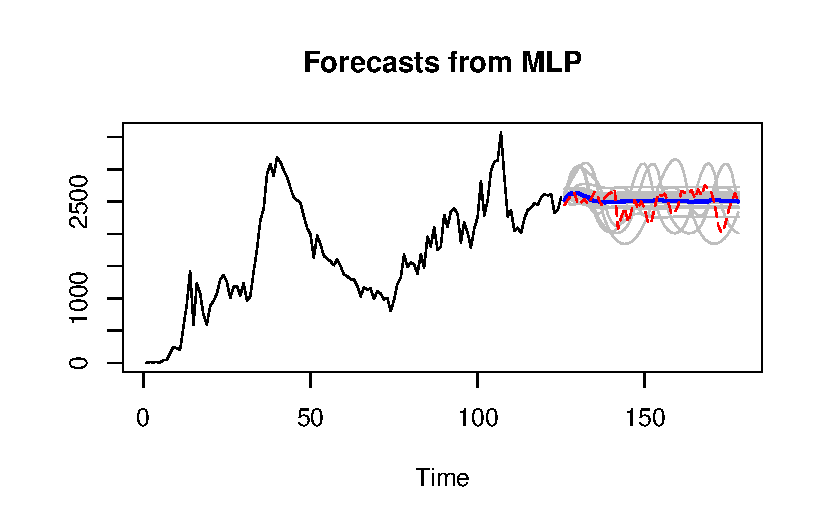
\includegraphics{confirmados_files/figure-pdf/unnamed-chunk-27-1.pdf}

}

\caption{\label{fig-foremlp}Predicción futura de la serie tiempo para
casos confirmados mediante el modelo MLP}

\end{figure}%

Los resultados del pronóstico indican que el 14 de septiembre de 2020 se
proyectan 2494 nuevos casos confirmados de COVID-19. Estos valores
correspondientes al período de 30 días se detallan a continuación en la
Tabla~\ref{tbl-treinta} .

\begin{table}

\caption{\label{tbl-treinta}Pronóstico de casos confirmados de COVID-19
en Irán en los próximos 30 días}

\centering{


\includegraphics{confirmados_files/figure-pdf/tbl-treinta-1.pdf}

}

\end{table}%

Todo este análisis se hizo con el fin de corroborar los resultados
obtenidos en (Talkhi et~al. 2021).

\chapter{Pronóstico de casos de muerte por COVID-19 en
Irán}\label{pronuxf3stico-de-casos-de-muerte-por-covid-19-en-iruxe1n}

De manera similar a la evaluación llevada a cabo en la base de datos de
los casos confirmados de COVID-19 en Irán, se ejecutó un análisis para
los datos de muertes por COVID-19 en Irán, abarcando el mismo período
temporal, desde el 20 de febrero hasta el 15 de agosto de 2020. El
propósito fue determinar si, de forma análoga, la red neuronal MLP
demuestra un mejor ajuste a los datos en comparación con la técnica de
series temporales Holt-Winters, o si, en este caso particular, la
técnica Holt-Winters ofrece una mayor precisión.

Es relevante señalar la presencia de datos faltantes para las fechas 21
de febrero, 1 de marzo y 5 de mayo de 2020 en el conjunto de datos. Por
consiguiente, al igual que en los casos confirmados, se procedió con una
interpolación promedio para sustituir dichos datos faltantes. La
Figura~\ref{fig-muertes} exhibe la serie temporal resultante luego de
estas correcciones.

\begin{figure}

\centering{

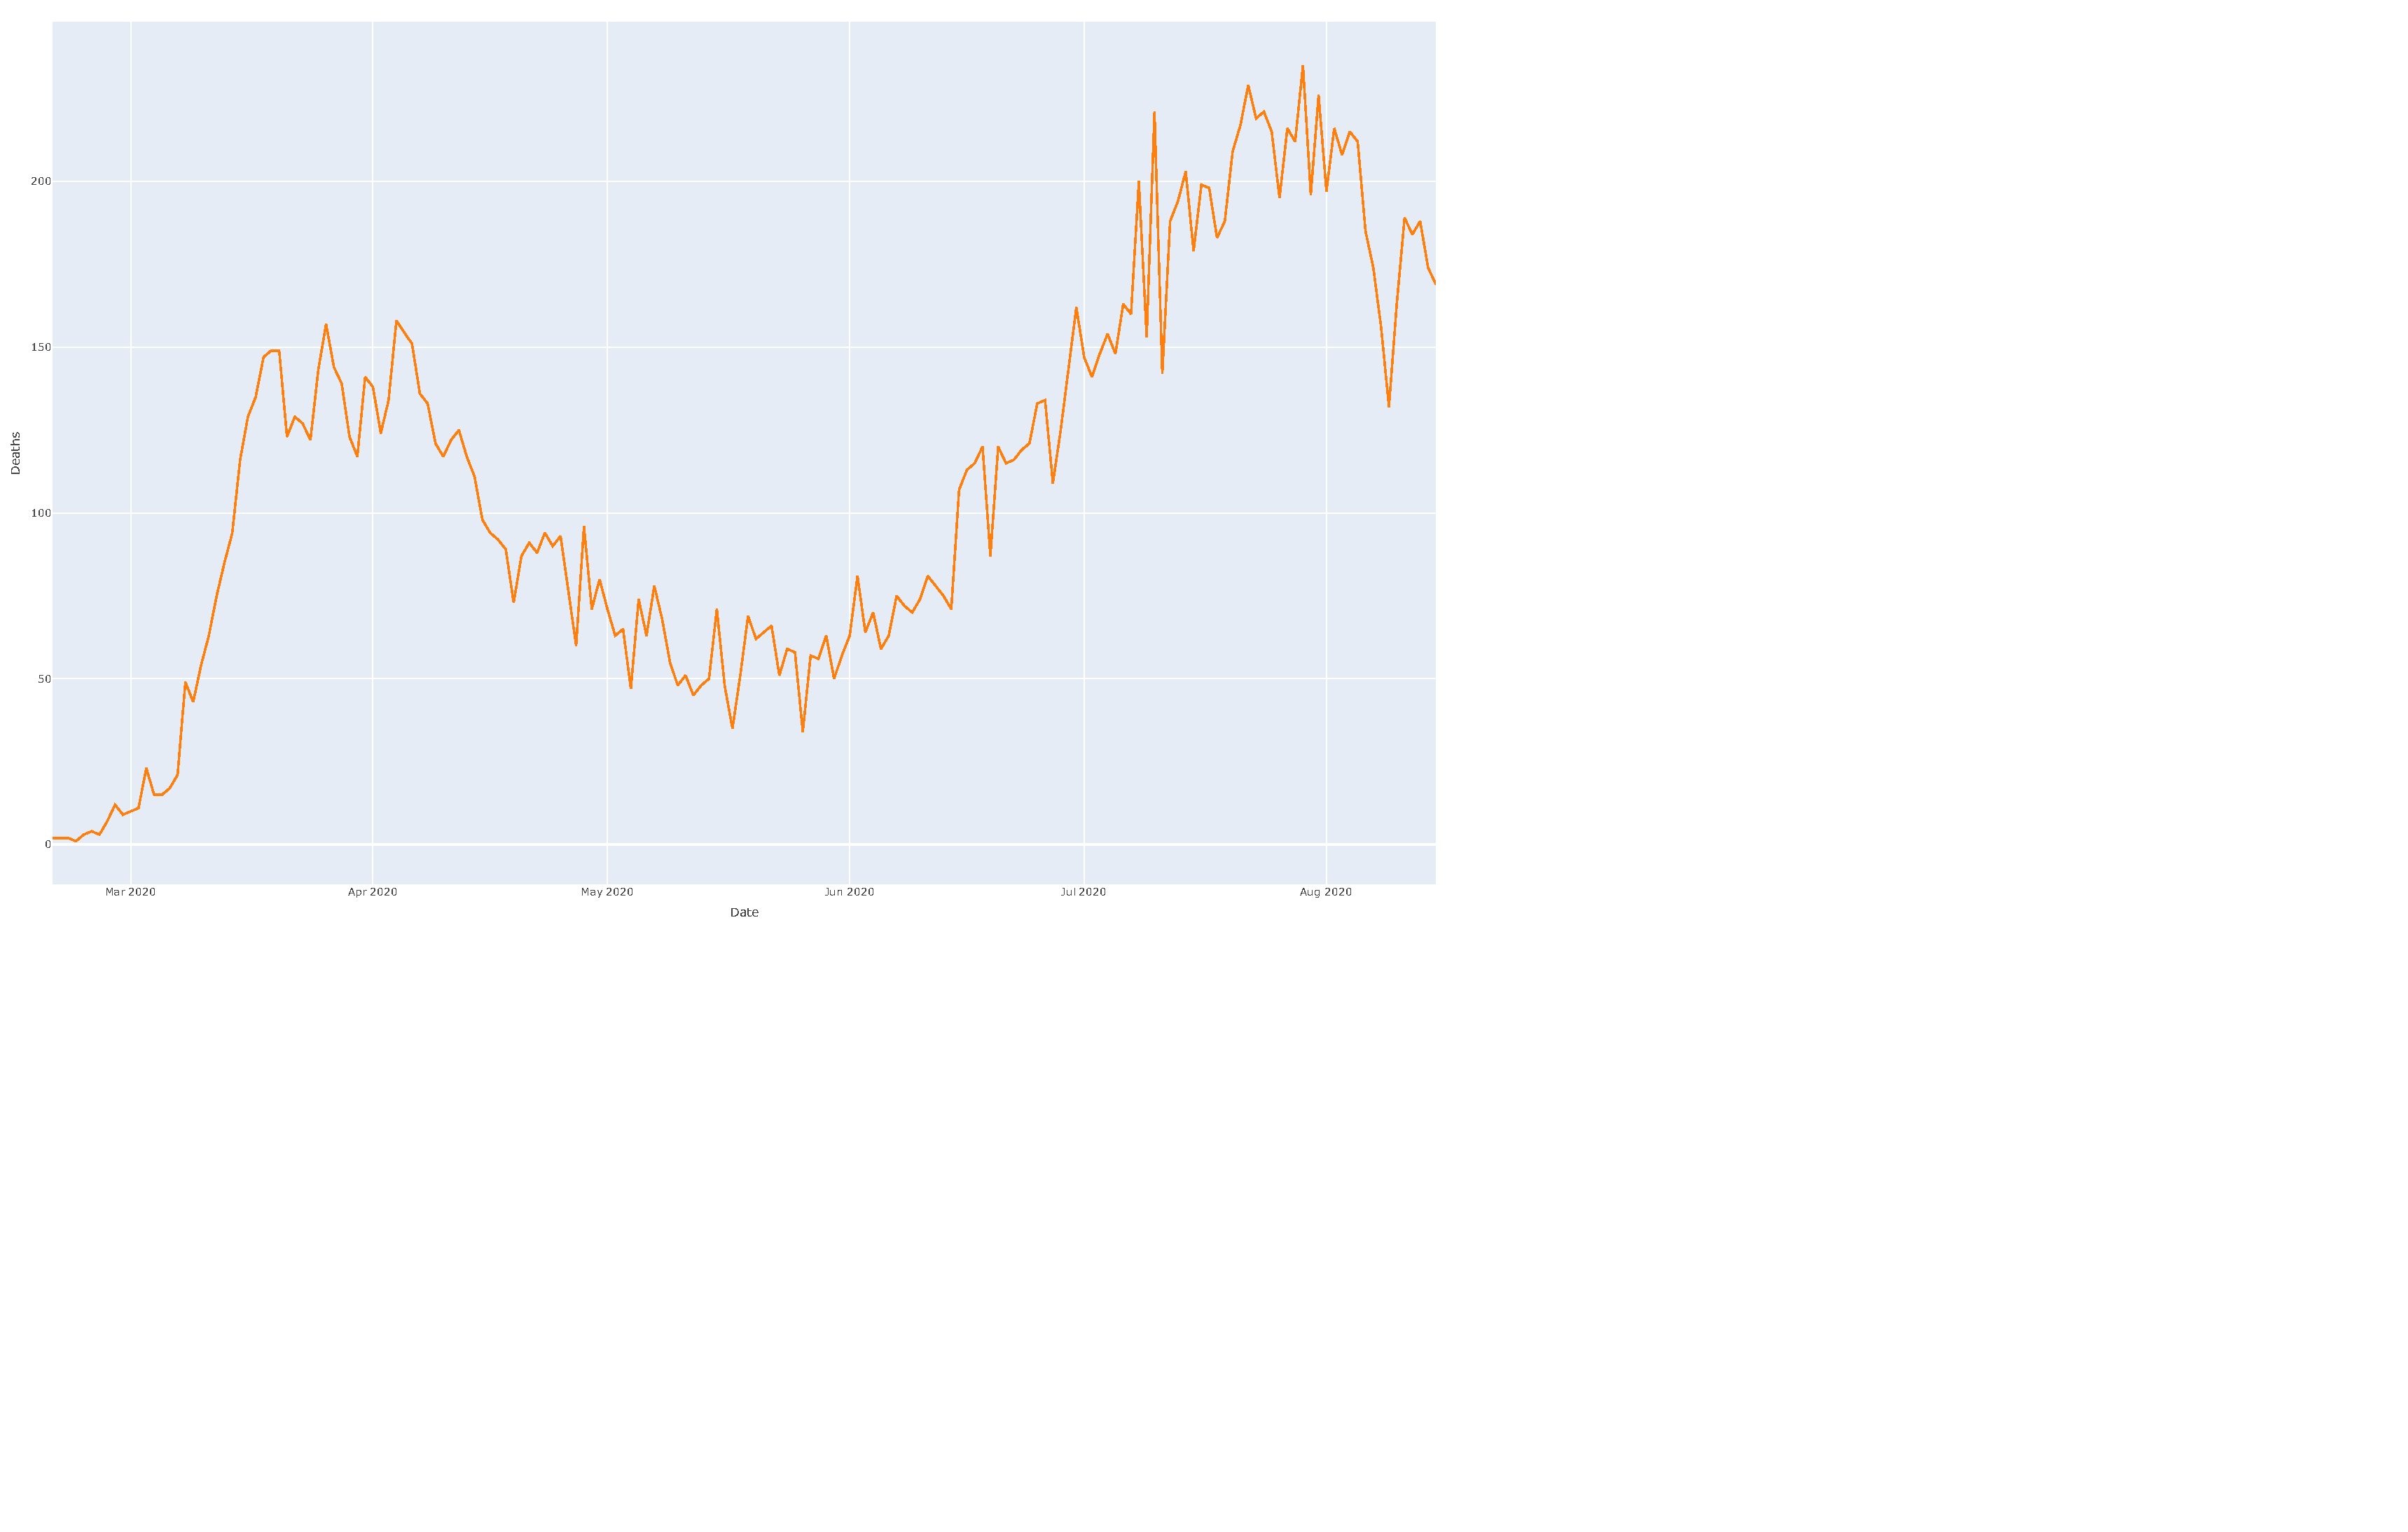
\includegraphics{muertes_files/figure-pdf/unnamed-chunk-3-1.pdf}

}

\caption{\label{fig-muertes}Serie de tiempo de los casos de muerte por
COVID-19 en Irán del 20-02-2020 al 15-08-2020}

\end{figure}%

\section{Pronóstico, comparación y métricas de
rendimiento}\label{pronuxf3stico-comparaciuxf3n-y-muxe9tricas-de-rendimiento}

La evaluación del desempeño de los métodos se realiza a través de la
separación del conjunto de datos en entrenamiento y prueba. El set
inicial, compuesto por el \(70\%\) de los datos, se emplea para el
entrenamiento de los modelos, mientras que el \(30\%\) restante se
reservará para llevar a cabo las pruebas pertinentes.

\begin{Shaded}
\begin{Highlighting}[]
\NormalTok{Deaths\_ts }\OtherTok{\textless{}{-}} \FunctionTok{ts}\NormalTok{(Deaths\_ts,}\AttributeTok{frequency=}\DecValTok{1}\NormalTok{) }
\NormalTok{tsize }\OtherTok{\textless{}{-}} \FunctionTok{round}\NormalTok{(}\FloatTok{0.7} \SpecialCharTok{*} \FunctionTok{nrow}\NormalTok{(Deaths\_df)) }
\NormalTok{train\_deaths }\OtherTok{\textless{}{-}} \FunctionTok{window}\NormalTok{(Deaths\_ts,}\AttributeTok{end=}\NormalTok{tsize) }
\NormalTok{test\_deaths }\OtherTok{\textless{}{-}} \FunctionTok{window}\NormalTok{(Deaths\_ts,}\AttributeTok{start=}\NormalTok{tsize}\SpecialCharTok{+}\DecValTok{1}\NormalTok{)}
\end{Highlighting}
\end{Shaded}

Con el propósito de llevar a cabo un análisis cuantitativo exhaustivo,
se presenta a continuación una tabla comparativa de los resultados
derivados de las dos técnicas implementadas (después de realizar el
entrenamiento, modelado y pronóstico), y la base de datos de prueba.
Posteriormente, se exhiben gráficas representativas de estos resultados.
En la Figura~\ref{fig-phwd} se muestra el pronóstico mediante
Holt-Winters acompañado de su respectivo intervalo de confianza. En
contraste, en la Figura~\ref{fig-pmlpd}, la gráfica punteada en color
rojo representa el comportamiento real de los datos, mientras que en
azul se representa el pronóstico obtenido a través de la red MLP.

\begin{table}

\caption{\label{tbl-forecastd}Comparación de Resultados entre las
técnicas y los datos reales para evaluar precisión}

\centering{


\includegraphics{muertes_files/figure-pdf/tbl-forecastd-1.pdf}

}

\end{table}%

\begin{figure}

\centering{

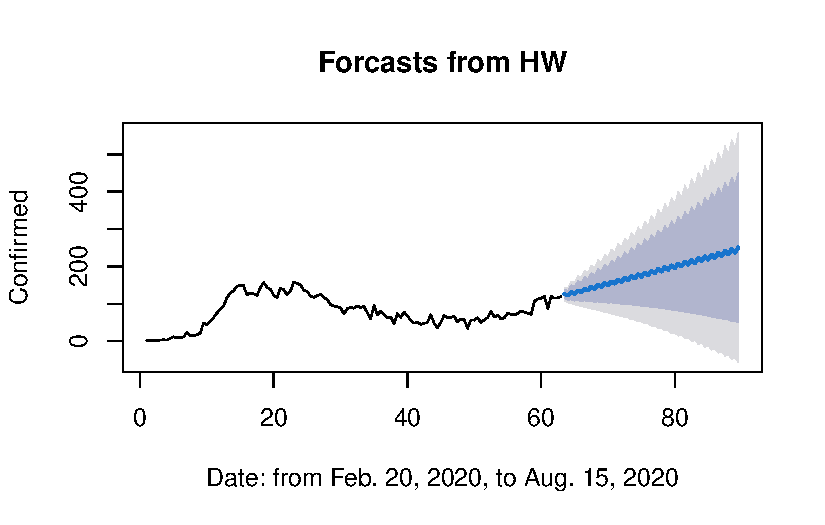
\includegraphics{muertes_files/figure-pdf/unnamed-chunk-7-1.pdf}

}

\caption{\label{fig-phwd}Pronóstico obtenido mediante la técnica de
Holt-Winters.}

\end{figure}%

\begin{figure}

\centering{

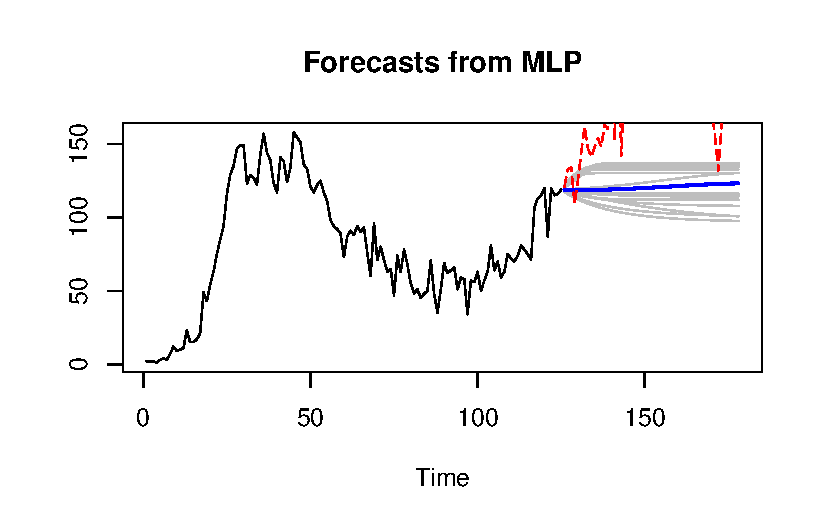
\includegraphics{muertes_files/figure-pdf/unnamed-chunk-8-1.pdf}

}

\caption{\label{fig-pmlpd}Pronóstico obtenido mediante la red neuronal
MLP.}

\end{figure}%

Utilizando las métricas establecidas en Ecuación~\ref{eq-metricas}, se
lleva a cabo la evaluación de la calidad o bondad de ajuste de los
métodos empleados en este estudio con el fin de seleccionar el modelo
más adecuado.

\begin{longtable}[]{@{}
  >{\raggedright\arraybackslash}p{(\columnwidth - 12\tabcolsep) * \real{0.1810}}
  >{\centering\arraybackslash}p{(\columnwidth - 12\tabcolsep) * \real{0.1143}}
  >{\centering\arraybackslash}p{(\columnwidth - 12\tabcolsep) * \real{0.1619}}
  >{\centering\arraybackslash}p{(\columnwidth - 12\tabcolsep) * \real{0.1143}}
  >{\centering\arraybackslash}p{(\columnwidth - 12\tabcolsep) * \real{0.1143}}
  >{\centering\arraybackslash}p{(\columnwidth - 12\tabcolsep) * \real{0.1524}}
  >{\centering\arraybackslash}p{(\columnwidth - 12\tabcolsep) * \real{0.1143}}@{}}
\caption{Errores de los modelos para casos
confirmados.}\label{tbl-errd}\tabularnewline
\toprule\noalign{}
\endfirsthead
\endhead
\bottomrule\noalign{}
\endlastfoot
& & \textbf{\emph{Training}} & & & \textbf{\emph{Testing}} & \\
& \textbf{RMSE} & \textbf{MAE} & \textbf{MAPE} & \textbf{RMSE} &
\textbf{MAE} & \textbf{MAPE} \\
\textbf{Holt-Winters} & \emph{12.6365} & \emph{9.6103} & \emph{19.4096}
& \emph{34.0665} & \emph{25.5356} & \emph{12.9770} \\
\textbf{MLP} & \emph{11.7584} & \emph{8.8446} & \emph{15.6144} &
\emph{67.2031} & \emph{59.7811} & \emph{49.0686} \\
\end{longtable}

Los resultados derivados de la tabla de errores (Tabla~\ref{tbl-errd})
llevan a la conclusión de que, en esta base de datos específica, a pesar
de que la red MLP exhibe errores más reducidos durante la fase de
entrenamiento, la técnica de Holt-Winters presenta un error
considerablemente menor en la etapa de prueba en comparación con MLP.
Esto evidencia su mayor eficacia en la predicción realizada. Por
consiguiente, se recomienda el uso del método Holt-Winters para llevar a
cabo el pronóstico de los próximos 30 días.

\section{Pronóstico de los próximos 30
días}\label{pronuxf3stico-de-los-pruxf3ximos-30-duxedas-1}

\begin{Shaded}
\begin{Highlighting}[]
\CommentTok{\#predicciones por medio de HW de los datos originales }
\NormalTok{HW\_deaths }\OtherTok{\textless{}{-}} \FunctionTok{HoltWinters}\NormalTok{(}\FunctionTok{ts}\NormalTok{(Deaths\_df}\SpecialCharTok{$}\NormalTok{Deaths,}\AttributeTok{frequency =} \DecValTok{2}\NormalTok{)) }
\CommentTok{\#Realizamos predicciones con h=30 (30 días) con nivel de confianza para los \#intervalos de predicción de 80 a 95\% }
\NormalTok{HW\_for\_d }\OtherTok{\textless{}{-}} \FunctionTok{forecast}\NormalTok{(HW\_deaths, }\AttributeTok{h=}\DecValTok{30}\NormalTok{, }\AttributeTok{level=}\FunctionTok{c}\NormalTok{(}\DecValTok{80}\NormalTok{,}\DecValTok{95}\NormalTok{)) }
\FunctionTok{plot}\NormalTok{(HW\_for\_d)  }
\end{Highlighting}
\end{Shaded}

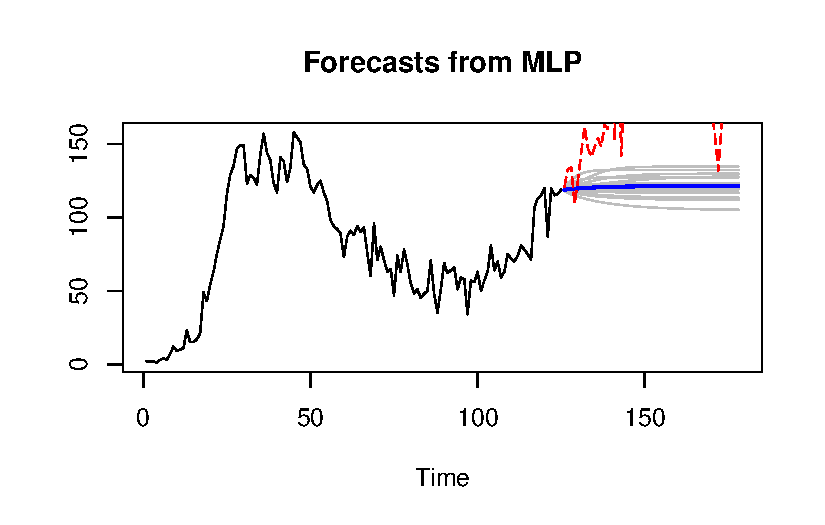
\includegraphics{muertes_files/figure-pdf/unnamed-chunk-10-1.pdf}

\begin{Shaded}
\begin{Highlighting}[]
\CommentTok{\#Predicciones por medio de MLP de los datos originales }
\NormalTok{fit.mlp\_d }\OtherTok{=} \FunctionTok{mlp}\NormalTok{(}\FunctionTok{ts}\NormalTok{(Deaths\_df}\SpecialCharTok{$}\NormalTok{Deaths),}\AttributeTok{reps =} \DecValTok{20}\NormalTok{,}\AttributeTok{hd.auto.type =} \StringTok{\textquotesingle{}cv\textquotesingle{}}\NormalTok{,}\AttributeTok{comb=}\StringTok{"median"}\NormalTok{) }\CommentTok{\#Realizamos predicciones con h=30 (30 días) }
\NormalTok{fore.mlp\_d }\OtherTok{=} \FunctionTok{forecast}\NormalTok{(fit.mlp\_d, }\AttributeTok{h =} \DecValTok{30}\NormalTok{) }
\FunctionTok{plot}\NormalTok{(fore.mlp\_d)}
\end{Highlighting}
\end{Shaded}

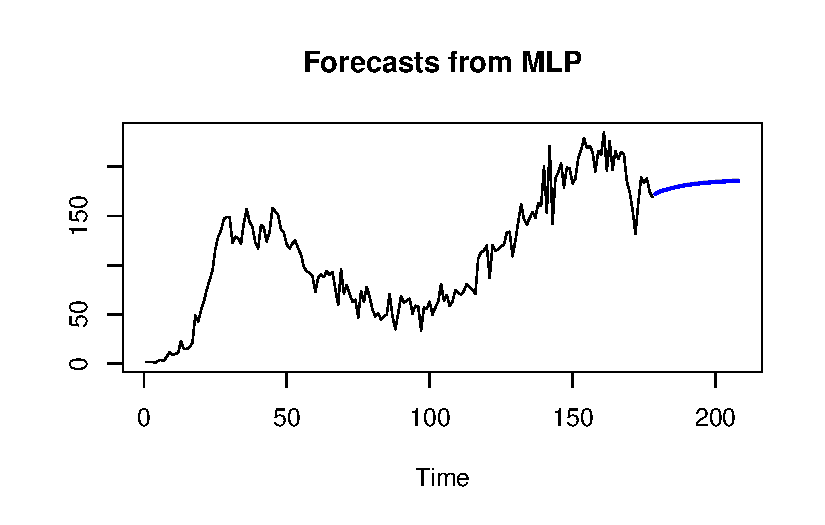
\includegraphics{muertes_files/figure-pdf/unnamed-chunk-10-2.pdf}

\bookmarksetup{startatroot}

\chapter*{References}\label{references}
\addcontentsline{toc}{chapter}{References}

\markboth{References}{References}

\phantomsection\label{refs}
\begin{CSLReferences}{1}{0}
\bibitem[\citeproctext]{ref-ash2000probability}
Ash, R. B., y C. A. Doleans-Dade. 2000. \emph{Probability and Measure
Theory}. Elsevier Science.
\url{https://books.google.com.mx/books?id=GkqQoRpCO2QC}.

\bibitem[\citeproctext]{ref-castauxf1eda2014introduction}
Castañeda, L. B., V. Arunachalam, y S. Dharmaraja. 2014.
\emph{Introduction to Probability and Stochastic Processes with
Applications}. Wiley.
\url{https://books.google.com.mx/books?id=M0hYBAAAQBAJ}.

\bibitem[\citeproctext]{ref-holt1957forecasting}
Holt, Charles C. 1957. {«Forecasting trends and seasonals by
exponentially weighted moving averages»}. \emph{ONR Memorandum} 52 (52):
5-10.

\bibitem[\citeproctext]{ref-joseph1961contributions}
Joseph, Roger David. 1961. \emph{Contributions to perceptron theory}.
Cornell University.

\bibitem[\citeproctext]{ref-knuth84}
Knuth, Donald E. 1984. {«Literate Programming»}. \emph{Comput. J.} 27
(2): 97-111. \url{https://doi.org/10.1093/comjnl/27.2.97}.

\bibitem[\citeproctext]{ref-nnfor}
Kourentzes, Nikolaos. 2022. {«nnfor: Time Series Forecasting with Neural
Networks»}. \url{https://CRAN.R-project.org/package=nnfor}.

\bibitem[\citeproctext]{ref-lipschutz1996probabilidad}
Lipschutz, S. 1996. \emph{Probabilidad}. McGraw-Hill.
\url{https://books.google.com.mx/books?id=vndlwgEACAAJ}.

\bibitem[\citeproctext]{ref-mann2010introductory}
Mann, P. S. 2010. \emph{Introductory Statistics}. John Wiley \& Sons.
\url{https://books.google.com.mx/books?id=N_mEBiCYaqkC}.

\bibitem[\citeproctext]{ref-mcculloch1943logical}
McCulloch, Warren S, y Walter Pitts. 1943. {«A logical calculus of the
ideas immanent in nervous activity»}. \emph{The bulletin of mathematical
biophysics} 5: 115-33.

\bibitem[\citeproctext]{ref-mood1986introduction}
Mood, A. M. F., F. A. Graybill, y D. C. Boes. 1986. \emph{Introduction
to the Theory of Statistics}. McGraw-Hill series en Probability y
Statistics. \url{https://books.google.com.mx/books?id=bKHBjgEACAAJ}.

\bibitem[\citeproctext]{ref-stats}
R Core Team. 2023. {«R: A Language and Environment for Statistical
Computing»}. \url{https://www.R-project.org/}.

\bibitem[\citeproctext]{ref-rosenblatt1960perceptron}
Rosenblatt, Frank. 1960. {«Perceptron simulation experiments»}.
\emph{Proceedings of the IRE} 48 (3): 301-9.

\bibitem[\citeproctext]{ref-ross1995stochastic}
Ross, S. M. 1995. \emph{Stochastic Processes}. Wiley series en
probability y mathematical statistics. Wiley.
\url{https://books.google.com.mx/books?id=qiLdCQAAQBAJ}.

\bibitem[\citeproctext]{ref-talkhi2021modeling}
Talkhi, Nasrin, Narges Akhavan Fatemi, Zahra Ataei, y Mehdi Jabbari
Nooghabi. 2021. {«Modeling and forecasting number of confirmed and death
caused COVID-19 in IRAN: A comparison of time series forecasting
methods»}. \emph{Biomedical signal processing and control} 66: 102494.

\bibitem[\citeproctext]{ref-winters1960forecasting}
Winters, Peter R. 1960. {«Forecasting sales by exponentially weighted
moving averages»}. \emph{Management science} 6 (3): 324-42.

\bibitem[\citeproctext]{ref-woodward2022time}
Woodward, W. A., B. P. Sadler, y S. Robertson. 2022. \emph{Time Series
for Data Science: Analysis and Forecasting}. A Chapman \& Hall Book. CRC
Press, Taylor \& Francis Group.
\url{https://books.google.com.mx/books?id=gM3gzgEACAAJ}.

\end{CSLReferences}



\end{document}
